%   MSc Business Analytics Dissertation
%
%   Title:     The Relationship Between Corporate Governance and Company Performance
%   Author: Conor Reid 
%
%   Chapter 4: Results
%

\chapter{Results}\label{C.Results}

\section{Introduction}\label{S.intro4}
{This chapter outlines the results of each stage of this study. First, results from the replication of the work of \cite{moldovan2015learning} are shown, who modelled the problem as a classification exercise by thresholding on the continuous, success measuring dependant variables. Next, regression results are presented which are obtained by neglecting that thresholding. Finally, causal estimation results are presented which are obtained by implementing propensity score matching, using those findings as the basis for research questions. \\\\
Below, some summary statistics are presented on the dependent variables used in this study. This is so as to provide a reference point for analysing the results below, particularity the regression results which list the RMSE (root mean square error) which is in the same units as the dependant variable involved. 
\begin{table}[h!]
\scalebox{0.9}{
\begin{tabular}{ |p{5.2cm}||p{1.2cm}|p{1.4cm}|p{1.5cm}|p{1.2cm}|p{1.4cm}|p{1.2cm}|  }
 \hline
 \multicolumn{7}{|c|}{\bf Tobin's Q Score} \\
  \hline
 {\bf Market} & {\bf Min} & {\bf \footnotesize 1st Qu.} & {\bf Median} & {\bf Mean } & {\bf \footnotesize 3rd Qu. } & {\bf Max.}  \\
 \hline
 S\&P 500 &0.8268 &  1.2670&  1.7490&  2.1760&  2.5180&  9.6360   \\
 STOXX Europe 600 &0.7437 & 1.0630 & 1.4300  &1.9250 & 2.0810& 72.290   \\
 STOXX Eastern Europe 300 &0.3399 & 0.9335 & 1.0590 & 1.3540 & 1.4320 & 7.8870   \\
  \hline
\end{tabular}}
\end{table}

\begin{table}[h!]
\scalebox{0.9}{
\begin{tabular}{ |p{5.2cm}||p{1.3cm}|p{1.4cm}|p{1.5cm}|p{1.2cm}|p{1.4cm}|p{1.2cm}|  }
 \hline
 \multicolumn{7}{|c|}{\bf Altman Z Score} \\
  \hline
 {\bf Market} & {\bf Min} & {\bf \footnotesize 1st Qu.} & {\bf Median} & {\bf Mean } & {\bf \footnotesize 3rd Qu. } & {\bf Max.}  \\
 \hline
 S\&P 500 &-9.896  & 2.450 &  4.026 &  4.562 &  5.372 & 28.480   \\
 STOXX Europe 600 &-0.6806 & 2.2150 & 3.3420 & 4.3980 & 5.0350 & 46.510   \\
 STOXX Eastern Europe 300 & -1.994 &  1.880 &  2.816 &  3.447 &  4.225 & 24.250   \\
  \hline
\end{tabular}}
\end{table}
\vspace{2cm}
\begin{table}[h!]
\scalebox{0.9}{
\begin{tabular}{ |p{2cm}||p{2.5cm}|p{1.3cm}|p{1.4cm}|p{1.5cm}|p{1.2cm}|p{1.4cm}|p{1.2cm}|  }
 \hline
 \multicolumn{8}{|c|}{\bf Benish M Score} \\
  \hline
 {\bf Market} & {{\bf Version}} & {\bf Min} & {\bf \footnotesize 1st Qu.} & {\bf Median} & {\bf Mean } & {\bf \footnotesize 3rd Qu. } & {\bf Max.}  \\
 \hline
 S\&P 500 & Eight Var & -8.905 & -2.829 & -2.634 & -2.660 & -2.471  & 0.000      \\
 S\&P 500 & Five Var & -13.720 & -3.013 & -2.918 & -2.903 & -2.775 &  0.525    \\ 
  \hline
\end{tabular}}
\end{table}}
\section{Classification}\label{S.classification4}
{For the classification portion of this study, two of the most performant algorithms used by \cite{moldovan2015learning} are implemented. For each dataset and algorithm, the original results are presented alongside the results of this study as a direct comparision. Include also are results obtained from an identical analysis but with outliers left in the dataset rather than removing them. This is discussed in section \ref{outliers}. For the S\&P, results are also presented that relate to identical analysis but with extra covariates included, as outlined in section \ref{NewFactors_Independent}.   }\clearpage
\subsection*{S\&P 500}
{Below, the results for the S\&P market are shown. Note that the original study removed outliers before modelling, and so it should be assumed that the current study did likewise unless otherwise stated.   }
\begin{table}[h!]
\centering
\begin{sideways}% 
\begin{tabular}{ |p{2.2cm}|p{1.55cm}|p{2.8cm}||p{2cm}|p{1.8cm}|p{1.8cm}|p{1cm}|  }
 \hline
 \multicolumn{7}{|c|}{\bf Dependent Variable : Tobin's Q Score} \\
 \hline
 {\bf Algorithm} & {\bf Study} & {\bf Modifier} & {\bf Accuracy (\%)} & {\bf Precision Class 0} & {\bf Precision Class 1} & {\bf ROC} \\
 \hline
   Adaboost & M\&M & - &  89.7177 & 0.890 &  0.905 & 0.957  \\
   \rowcolor{gray} Adaboost & Current & - & 92.1213  & 0.948 & 0.897 &  0.922 \\
   Adaboost & Current & With Outliers & 93.3734  & 0.950 & 0.915  &  0.933 \\
   \rowcolor{gray} Adaboost & Current & Extra Variables & 94.5783  & 0.962 & 0.931 &  0.947 \\
 & & & & & &\\
 J48  & M\&M & - & 85.2823  & 0.841 &  0.866 & 0.854  \\
  \rowcolor{gray} J48 (C5.0) & Current & - & 87.9519  & 0.886 & 0.871  & 0.879  \\
 J48 (C5.0)  & Current & With Outliers  &87.9518  & 0.840 & 0.930  & 0.885  \\
 \rowcolor{gray} J48 (C5.0) & Current & Extra Variables & 89.7590  & 0.951 & 0.847 &  0.899 \\
 \hline
\end{tabular}
\end{sideways}
\caption{Classification Results - S\&P 500, Tobin's Q Score}
\end{table}

\begin{table}[h]
\centering
\begin{sideways}% 
\begin{tabular}{ |p{2.2cm}|p{1.55cm}|p{2.8cm}||p{2cm}|p{2cm}|p{2cm}|p{2cm}|p{1cm}|  }
 \hline
 \multicolumn{8}{|c|}{\bf Dependent Variable : Altman Z Score} \\
 \hline
{\bf Algorithm} & {\bf Study} & {\bf Modifier} & {\bf Accuracy (\%)} & {\bf Precision Class 0} & {\bf Precision Class 1} &{\bf  Precision Class 2} & {\bf ROC} \\
 \hline
  Adaboost  & M\&M  & - &  82.944     & 0.843 &  0.725 & 0.865 & 0.942  \\
  \rowcolor{gray}Adaboost & Current & - & 83.3334 & 0.818 & 0.348  & 0.957 & 0.879  \\
  Adaboost & Current & With Outliers & 84.892 & 0.818 & 0.529  & 0.910  & 0.861  \\
  \rowcolor{gray}Adaboost & Current & Extra Variables & 88.4892 & 0.882 & 0.6  & 0.925  & 0.871  \\

  & & & & & & &\\
 J48  & M\&M & - &73.6086  & 0.722 &  0.569 & 0.816 & 0.843  \\
 \rowcolor{gray}J48 (C5.0) & Current & - &78.985 & 0.629 & 0.400  & 0.871 &  0.802 \\
 J48 (C5.0) & Current & With Outliers &81.2949 & 0.591 & 0.529 & 0.910  &  0.832 \\
 \rowcolor{gray}J48 (C5.0) & Current & Extra Variables & 76.978  & 0.6 & 0.485 & 0.928  & 0.831   \\
 \hline
\end{tabular}
\end{sideways}
\caption{Classification Results  - S\&P 500, Altman Z Score}
\end{table}
\clearpage
{Shown below is a sample decision tree, constructed by the C5.0 (equivalent to J48) for the Altman Z score. This was constructed using the auxiliary features included in this study. Although those variables do not drastically influence the aggregate model performance (as shown by the tables above), the social disclosure score interestingly appears near the bottom and is assigned an importance of 5\% by the algorithm. }\\
%\begin{lstlisting}[
%    basicstyle=\tiny, %or \small or \footnotesize etc.
%    caption={J48 - S\&P with Extra Variables for Altman Z Score - Decision Tree},
%    captionpos=b,
%    label={sampleDT}
%]
%Asset <= 0.4571385:
%:...Fincl..l <= 1.938166:
%:   :...P.B <= 2.182174: grey (8)
%:   :   P.B > 2.182174: safe (6.1/0.1)
%:   Fincl..l > 1.938166:
%:   :...X..Indep.Directors <= 84.62:
%:       :...EPS > 4.76: grey (2)
%:       :   EPS <= 4.76:
%:       :   :...P.B <= 2.246135: distress (5)
%:       :       P.B > 2.246135: safe (7.2/0.2)
%:       X..Indep.Directors > 84.62:
%:       :...Dvd.Yld > 2.724871: distress (23)
%:           Dvd.Yld <= 2.724871:
%:           :...Oper.ROE <= 9.037546: distress (7)
%:               Oper.ROE > 9.037546:
%:               :...Fincl..l <= 5.621416: grey (6)
%:                   Fincl..l > 5.621416: distress (2)
%Asset > 0.4571385:
%:...Interest <= 74.38541:
%    :...Board.Mtgs.. <= 6: safe (5/1)
%    :   Board.Mtgs.. > 6:
%    :   :...Sz.Aud.Cmte <= 3: distress (2.1/1)
%    :       Sz.Aud.Cmte > 3:
%    :       :...X..Feml.Execs.1 <= 0: distress (2.1/0.1)
%    :           X..Feml.Execs.1 > 0: grey (8/1)
%    Interest > 74.38541:
%    :...Fincl..l <= 3.202927:
%        :...X5Yr.Avg.Adj.ROE > 13.8612: safe (116.1/1.6)
%        :   X5Yr.Avg.Adj.ROE <= 13.8612:
%        :   :...X..Wmn.on.Bd <= 3: safe (32.4/4.5)
%        :       X..Wmn.on.Bd > 3: grey (2)
%        Fincl..l > 3.202927:
%        :...Asset <= 0.6752533:
%            :...OPM.T12M <= 18.86604: distress (5)
%            :   OPM.T12M > 18.86604: grey (3.1)
%            Asset > 0.6752533:
%            :...EV.EBITDA.T12M <= 4.797605: distress (2)
%                EV.EBITDA.T12M > 4.797605:
%                :...Indep.Directors <= 9: safe (19.8/0.1)
%                    Indep.Directors > 9:
%                    :...SOCIAL_DISCLOSURE_SCORE <= 28.0702: grey (3.2)
%                        SOCIAL_DISCLOSURE_SCORE > 28.0702: safe (9/1)
                     
%\end{lstlisting}
%\clearpage

\begin{figure}[h!]\label{sampleDT}
\centering
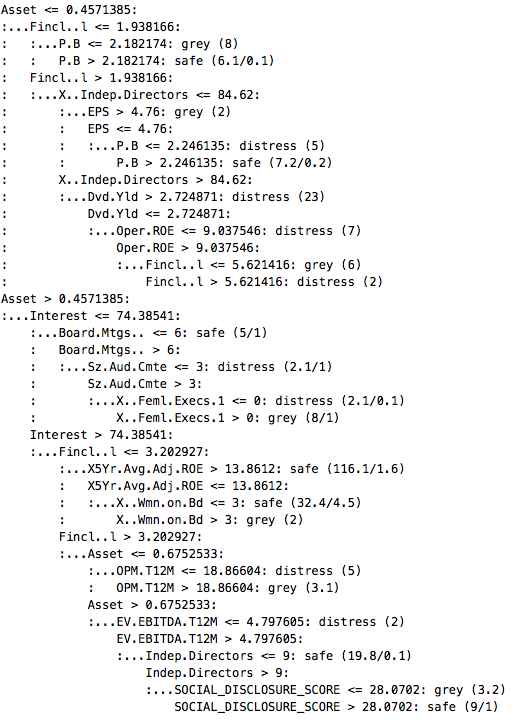
\includegraphics[scale=0.55]{images/sampleDT}
\caption{J48 - S\&P with Extra Variables for Altman Z Score - Decision Tree}
\end{figure}




\clearpage
\subsection*{STOXX Europe 600}
{Below, the results for the STOXX Europe 600 index are shown. Note that the auxiliary variables mentioned in section \ref{NewFactors_Independent} and \ref{NewFactors_Dependent} were not gathered for this index. }
\begin{table}[h!]
\centering
\begin{sideways}% 
\begin{tabular}{ |p{2.2cm}|p{1.55cm}|p{2.8cm}||p{2cm}|p{1.8cm}|p{1.8cm}|p{1cm}|  }
 \hline
 \multicolumn{7}{|c|}{\bf Dependent Variable : Tobin's Q Score} \\
 \hline
 {\bf Algorithm} & {\bf Study} & {\bf Modifier} & {\bf Accuracy (\%)} & {\bf Precision Class 0} & {\bf Precision Class 1} & {\bf ROC} \\
 \hline
  Adaboost  & M\&M & - & 88.2353     & 0.891 &  0.874 & 0.946  \\
  \rowcolor{gray}Adaboost & Current & - &94.4723  & 0.961 & 0.929 & 0.945 \\
  Adaboost & Current & With Outliers &90.9547 & 0.904 & 0.916  & 0.910  \\
 & & & & & & \\
 \rowcolor{gray}J48  & M\&M & - &87.395  & 0.871 &  0.877 & 0.874  \\
  J48 (C5.0) & Current & - &89.9497  & 0.915 & 0.884 & 0.900 \\
 \rowcolor{gray}J48 (C5.0)  & Current & With Outliers &87.940 & 0.887 &  0.873 &  0.879 \\
 \hline
\end{tabular}
\end{sideways}
\caption{Classification Results - STOXX Europe 600, Tobin's Q Score}
\end{table}

\begin{table}[h]
\centering
\begin{sideways}% 
\begin{tabular}{ |p{2.2cm}|p{1.55cm}|p{2.5cm}||p{2cm}|p{2cm}|p{2cm}|p{2cm}|p{1cm}|  }
 \hline
 \multicolumn{8}{|c|}{\bf Dependent Variable : Altman Z Score} \\
 \hline
 {\bf Algorithm} & {\bf Study} & {\bf Modifier} & {\bf Accuracy (\%)} & {\bf Precision Class 0} & {\bf Precision Class 1} &  {\bf Precision Class 2} & {\bf ROC} \\
 \hline
  Adaboost & M\&M & - & 76.2681  & 0.804 &  0.522 & 0.864 & 0.769  \\
  \rowcolor{gray}Adaboost & Current & - & 82.1656 & 0.793 & 0.692  & 0.887 & 0.895  \\
  Adaboost & Current & With Outliers & 77.0709 & 0.758 & 0.591 &  0.869 & 0.874  \\
  & & & & & & &\\
 \rowcolor{gray}J48  & M\&M & - & 74.2754  & 0.788 &  0.531 & 0.803 & 0.856  \\
  J48 (C5.0) & Current & - &  66.8789 & 0.75 & 0.369  & 0.804 & 0.798  \\
 \rowcolor{gray}J48  (C5.0) & Current & With Outliers & 69.4267 & 0.72 & 0.4318 & 0.8182  & 0.8243  \\

 \hline
\end{tabular}
\end{sideways}
\caption{Classification Results  - STOXX Europe 600, Altman Z Score}
\end{table}



\clearpage
\subsection*{STOXX Eastern Europe 300}
{Finally, the results for the STOXX Eastern Europe 300 index are shown below. Again, the auxiliary variables mentioned in section \ref{NewFactors_Independent} and \ref{NewFactors_Dependent} were not gathered for this index.}
\begin{table}[h!]
\centering
\begin{sideways}% 
\begin{tabular}{ |p{2.1cm}|p{1.4cm}|p{2.5cm}||p{1.9cm}|p{1.8cm}|p{1.8cm}|p{1cm}|  }
 \hline
 \multicolumn{7}{|c|}{\bf Dependent Variable : Tobin's Q Score} \\
 \hline
 {\bf Algorithm} & {\bf Study} & {\bf Modifier} & {\bf Accuracy (\%)} & {\bf Precision Class 0} & {\bf Precision Class 1} & {\bf ROC} \\
 \hline
  Adaboost  & M\&M & - &  81.8182     & 0.823 &  0.813 & 0.889  \\
  \rowcolor{gray} Adaboost  & Current & - &84.8488  & 0.88  & 0.816 & 0.848 \\
  Adaboost  & Current & With Outliers &82.8282  & 0.826 & 0.829  & 0.828  \\
 & & & & & & \\
   \rowcolor{gray}J48  & M\&M & - &77.1044  & 0.783 &  0.760 & 0.836  \\
  J48 (C5.0) & Current & - &78.7879  & 0.7021 & 0.865  & 0.783  \\
  \rowcolor{gray} J48 (C5.0) & Current & With Outliers &81.8182  & 0.826  & 0.808  &  0.818 \\
 \hline
\end{tabular}
\end{sideways}
\caption{Classification Results - STOXX Eastern Europe 300, Tobin's Q Score}
\end{table}

\begin{table}[h]
\centering
\begin{sideways}% 
\begin{tabular}{ |p{2.2cm}|p{1.55cm}|p{2.5cm}||p{2cm}|p{2cm}|p{2cm}|p{2cm}|p{1cm}|  }
 \hline
 \multicolumn{8}{|c|}{\bf Dependent Variable : Altman Z Score} \\
 \hline
 {\bf Algorithm} & {\bf Study} & {\bf Modifier} & {\bf Accuracy (\%)} & {\bf Precision Class 0} & {\bf Precision Class 1} &  {\bf Precision Class 2} & {\bf ROC} \\
 \hline
 Adaboost  & M\&M & & 63.7602  & 0.746 &  0.496 & 0.675 & 0.771  \\
   \rowcolor{gray}Adaboost  & Current & - &58.974 & 0.50 & 0.36 & 0.714  & 0.781  \\
 Adaboost  & Current & With Outliers &75.641 & 0.500 & 0.482 &  0.936 & 0.821  \\
   & & & & & & &\\
    \rowcolor{gray}J48  & M\&M & - & 65.6676  & 0.79 &  0.615 & 0.598 & 0.8  \\
  J48 (C5.0) & Current & - &62.821 & 0.334 & 0.447  & 0.813  &  0.723 \\
    \rowcolor{gray}J48 (C5.0) & Current & With Outliers &70.5122 & 0.334 & 0.650  & 0.746 & 0.879  \\
 \hline
\end{tabular}
\end{sideways}
\caption{Classification Results  - STOXX Eastern Europe 300, Altman Z Score}
\end{table}









\clearpage
\section{Regression}\label{S.regression4}
{There are no results from the original study to directly compare the regression results to, and so they are presented stand-alone. Tables are broken down by market and dependant variable.  An indication is given, in the form of yellow highlighting, of the optimal $alpha$ value and thus the optimal mix of ridge and lasso regression for each results set.  }\clearpage
\subsection*{S\&P 500}
{Shown below are regression results for the S\&P 500 stock index. }
\begin{table}[h!]
\centering
\scalebox{0.9}{
\begin{tabular}{ |p{2.5cm}||p{4cm}|p{4cm}| }
 \hline
 \multicolumn{3}{|c|}{\bf Dependent Variable - Tobin's Q Score} \\
 \hline
 {\bf Alpha} & $\mathbf r^2$ & {\bf RMSE} \\
 \hline
 0 (Ridge) & 0.514504662287613 & 1.54335249821869 \\          
0.1 & 0.736922216718774 & 0.752106800916883\\
0.2 & 0.723096373541166 & 0.918016920932065\\
0.3 & 0.736780891632018 & 0.729876793419644\\
0.4 & 0.728597775405239 & 0.802518515140072\\
0.5 & 0.736648154658892 & 0.736084477965634\\
0.6 & 0.728370638237572 & 0.729268748938413\\
0.7 & 0.736782224916274 & 0.740975835009645\\
\rowcolor{yellow}0.8 & 0.737003712724359 & 0.757117048022052\\
0.9 & 0.143531162654549 & 1.94074213436316\\
1.0 (Lasso) & 0.724748692727598 & 0.730134780410399 \\
 \hline
\end{tabular}
}
\caption{Regression Results  - S\&P 500, Tobin's Q Score}
\end{table}

\begin{table}[h!]
\centering
\scalebox{0.9}{
\begin{tabular}{ |p{2.5cm}||p{4cm}|p{4cm}| }
 \hline
 \multicolumn{3}{|c|}{\bf Dependent Variable - Altman Z Score} \\
 \hline
 {\bf Alpha} & $\mathbf r^2$ & {\bf RMSE} \\
 \hline
0 (Ridge) & 0.372331817825629 & 13.7865694258794\\
0.1 & 0.512946605245459 & 10.1747805657968\\
0.2 & 0.478411885246279 & 10.4174275138483\\
0.3 & 0.512484854172808 & 10.3869701107608\\
0.4 & 0.478650059026158 & 9.85821851442949\\
\rowcolor{yellow}0.5 & 0.512396355841667 & 9.61495426389283\\
0.6 & 0.513129590937884 & 10.3182884065172\\
0.7 & 0.512360136424729 & 10.2731129074996\\
0.8 & 0.51296402797329 & 10.0251122703722\\
0.9 & 0.158067206245976 & 16.6297402971145\\
1 (Lasso) & 0.481696182985345 & 9.7934982676994\\
 \hline
\end{tabular}}
\caption{Regression Results  - S\&P 500, Altman Z Score}
\end{table}\clearpage

{The Benish MScore, a probabilistic indictor of intentional financial reporting fraud, was scraped for the S\&P 500 set of companies, the regression results for which are presented below. As mentioned previously, both eight variable and five variable versions were included in this analysis. Each is shown separately below.   }
\begin{table}[h!]
\centering
\scalebox{0.9}{
\begin{tabular}{ |p{2.5cm}||p{2.5cm}||p{4cm}|p{4cm}| }
 \hline
 \multicolumn{4}{|c|}{\bf Dependent Variable - Benish M-Score} \\
 \hline
 {\bf Version} &  {\bf Alpha} & $\mathbf r^2$ & {\bf RMSE} \\
 \hline
Eight Var&0 ( Ridge)&0.251555481058366&0.484013829347385 \\
\rowcolor{yellow}Eight Var&0.1&0.252608488775166&0.46535791024093 \\
Eight Var&0.2&0.24789844766805&0.468175452095253 \\
Eight Var&0.3&0.2198137766366&0.49415213706807 \\
Eight Var&0.4&0.249189763200139&0.465779130278631 \\
Eight Var&0.5&0.24549798240231&0.500453741652562 \\
Eight Var&0.6&0.249004530587714&0.470463109817926 \\
Eight Var&0.7&0.243925438107858&0.49064305638191 \\
Eight Var&0.8&0.249749421198673&0.481038667522551 \\
Eight Var&0.9&0.250291037515949&0.48584148244414 \\
Eight Var&1 (Lasso)&0.246306522467078&0.477759843928307 \\
 \hline
\rowcolor{yellow}Five Var&0 ( Ridge)&0.291732059704306&0.962571803318562 \\
Five Var&0.1&0.290985985078737&0.934920221885852 \\
Five Var&0.2&0.289997856384489&0.922163141720248 \\
Five Var&0.3&0.288128362377427&0.959393842374148 \\
Five Var&0.4&0.290435845389172&0.936954320855632 \\
Five Var&0.5&0.285369018902806&0.969059899849606 \\
Five Var&0.6&0.290276479666761&0.927261185661328 \\
Five Var&0.7&0.289285439066985&0.982050720561862 \\
Five Var&0.8&0.290876191983076&0.94214790269637 \\
Five Var&0.9&0.290922502141949&0.937690067080429 \\
Five Var&1 (Lasso)&0.290548584733936&0.949720674526324 \\
 \hline
\end{tabular}}
\caption{Regression Results  - S\&P 500, Benish M-Score}
\end{table}
\clearpage

\subsection*{STOXX Europe 600}
{Shown below are regression results for the STOXX Europe 600 stock index. }
\begin{table}[h!]
\centering
\scalebox{0.9}{
\begin{tabular}{ |p{2.5cm}||p{4cm}|p{4cm}| }
 \hline
 \multicolumn{3}{|c|}{\bf Dependent Variable - Tobins Q Score} \\
 \hline
 {\bf Alpha} & $\mathbf r^2$ & {\bf RMSE} \\
 \hline
\rowcolor{yellow}0 (Ridge) & 0.924245520228615 & 4.52752573635043\\
0.1 & 0.936820396581318 & 5.61364933389961\\
0.2 & 0.936272434248921 & 6.12198520884377\\
0.3 & 0.936184193929519 & 6.60733408752952\\
0.4 & 0.936486005016966 & 6.78628962380346\\
0.5 & 0.937847903413279 & 6.655449299569\\
0.6 & 0.935338676848096 & 6.88804707065998\\
0.7 & 0.937887391702568 & 7.08560490201231\\
0.8 & 0.935720858099178 & 7.04925327857539\\
0.9 & 0.935982694015804 & 7.14379996319223\\
1 (Lasso) & 0.935805655675326 & 7.19289948947667\\
 \hline
\end{tabular}}
\caption{Regression Results  - STOXX Europe 600, Tobin's Q Score}
\end{table}

\begin{table}[h!]
\centering
\scalebox{0.9}{
\begin{tabular}{ |p{2.5cm}||p{4cm}|p{4cm}| }
 \hline
 \multicolumn{3}{|c|}{\bf Dependent Variable - Altman Z Score} \\
 \hline
 {\bf Alpha} & $\mathbf r^2$ & {\bf RMSE} \\
 \hline
0 (Ridge) & 0.493776589092134 & 12.4040377499728\\
0.1 & 0.492009638562525 & 13.0187735752629\\
0.2 & 0.492487747960643 & 12.571232251759\\
0.3 & 0.493364660095417 & 12.8447464487333\\
0.4 & 0.495255261342842 & 12.8572572045948\\
0.5 & 0.443363098262155 & 16.167925121637\\
\rowcolor{yellow}0.6 & 0.49250064188208 & 12.408424237533\\
0.7 & 0.410969802370212 & 14.5362919598181\\
0.8 & 0.493903828085151 & 12.4931721421183\\
0.9 & 0.494432810764225 & 12.128503187072\\
1 (Lasso) & 0.494019676145083 & 12.1087103638653\\
 \hline
\end{tabular}}
\caption{Regression Results  - STOXX Europe 600, Altman Z Score}
\end{table}
\clearpage


\subsection*{STOXX Eastern Europe 300}
{Shown below are regression results for the STOXX Eastern Europe 300 stock index. }
\begin{table}[h!]
\centering
\scalebox{0.9}{
\begin{tabular}{ |p{2.5cm}||p{4cm}|p{4cm}| }
 \hline
 \multicolumn{3}{|c|}{\bf Dependent Variable - Tobins Q Score} \\
 \hline
 {\bf Alpha} & $\mathbf r^2$ & {\bf RMSE} \\
 \hline
0 (Ridge) & 0.704355214812389 & 0.498974752786726\\
0.1 & 0.694006623409445 & 0.53354739142002\\
\rowcolor{yellow}0.2 & 0.727564731166982 & 0.47859949878705\\
0.3 & 0.69625780677679 & 0.475553525491744\\
0.4 & 0.707544799542626 & 0.478664221197991\\
0.5 & 0.656609682843319 & 0.546502619727653\\
0.6 & 0.68326568451999 & 0.50410936532166\\
0.7 & 0.667251282563606 & 0.590747734679593\\
0.8 & 0.668367543398841 & 0.462386508939621\\
0.9 & 0.699087289610586 & 0.454557500864114\\
1 (Lasso) & 0.660904967486424 & 0.462774482588657\\
 \hline
\end{tabular}}
\caption{Regression Results  - STOXX Eastern Europe 300, Tobin's Q Score}
\end{table}

\begin{table}[h!]
\centering
\scalebox{0.9}{
\begin{tabular}{ |p{2.5cm}||p{4cm}|p{4cm}| }
 \hline
 \multicolumn{3}{|c|}{\bf Dependent Variable - Altman Z Score} \\
 \hline
 {\bf Alpha} & $\mathbf r^2$ & {\bf RMSE} \\
 \hline
0 (Ridge) & 0.497359901145225 & 7.4448320397538\\
0.1 & 0.521420102039222 & 7.63377981958334\\
0.2 & 0.479465764190985 & 8.27754797472766\\
0.3 & 0.503750477243543 & 7.70658821833145\\
0.4 & 0.503990128494823 & 7.86100761373032\\
\rowcolor{yellow}0.5 & 0.524032769294246 & 8.25112976717522\\
0.6 & 0.512202382858808 & 8.15220512063965\\
0.7 & 0.507649931007144 & 8.02131671759577\\
0.8 & 0.493904840655251 & 8.1278950336226\\
0.9 & 0.495564417663372 & 8.2173172609159\\
1 (Lasso) & 0.480490621105762 & 8.19196705962938\\
 \hline
\end{tabular}}
\caption{Regression Results  - STOXX Eastern Europe 300, Altman Z Score}
\end{table}



\clearpage
\section{Causal Estimation}\label{S.causal4}
{This section deals with results pertaining the the causal estimation stage of the current study. As mentioned before, causal estimation involves the selection of treatment and effect pairs, as well as covariates to control on. Results are presented with reference to these pairs and covariates, and reference back to the motivating statement made in the original study where appropriate (see section \ref{CausalEstimation-ResearchQuestions} for more detail). \\\\
Note that while all original findings are tied to specific markets, those findings were tested for all markets in this study. Therefore the motivating statement listed for a particular set of results below may not match the dataset to which it was originally assigned. In some cases it was not possible to achieve a sufficient matching rate for particular datasets, in others the estimates were insignificant or the 95\% CI crossed zero. In these cases, results are omitted because the aggregate direction of the effect cannot be determined.\\\\
Each result set is presented following a uniform template, as per section \ref{interpretationCausal}. 
%A header is given as an indication of the type of corporate governance features involved. The market for which the results relate is listed, followed by the dependent variable. The treatment is given in the form:
%\begin{equation}
%condition \quad ? \quad value \ if \ true \ : \ value \ if \ false
%\end{equation}
%After this the motivating statement from section \ref{CausalEstimation-ResearchQuestions} is given if applicable. In brackets here, an flag is given for whether the results below agree with the statement or not as well as whether this statement was originally made about this particular market or not ({\it original} or {\it not original}. This is purely to aid quick interpretation. The causal estimate as per the matching process is then given, as a 95\% confidence interval. Finally a series of plots are included showing the quality of that matching process on a covariate basis. }
\clearpage
\subsection{S\&P 500}
%%%%%%%%%%%%
%%Independent Director \& Financial Leverage
%%%%%%%%%%%%
\subsubsection{Independent Director \& Financial Leverage}
%\iffalse
\begin{tabular}{ll}
{\bf Market} & S\&P 500  \\
{\bf Outcome} & Altman Z Score \\
{\bf Treatment} & \footnotesize{(Indep Lead Dir \& Financial Leverage $>$ 2.5)? 1 : 0 } \\
{\bf Motivating Statement} & \ref{spTwo} [agrees, original]  \\
{\bf Estimate ($\% \Delta , 95\% \ CI$)} &  (-0.15 , -0.12 , -0.09) \\~\\
{\bf Matching Plots} &
\end{tabular}
\begin{figure}[h!]
\begin{tabular}{ccc}
\subfigure[Asset]{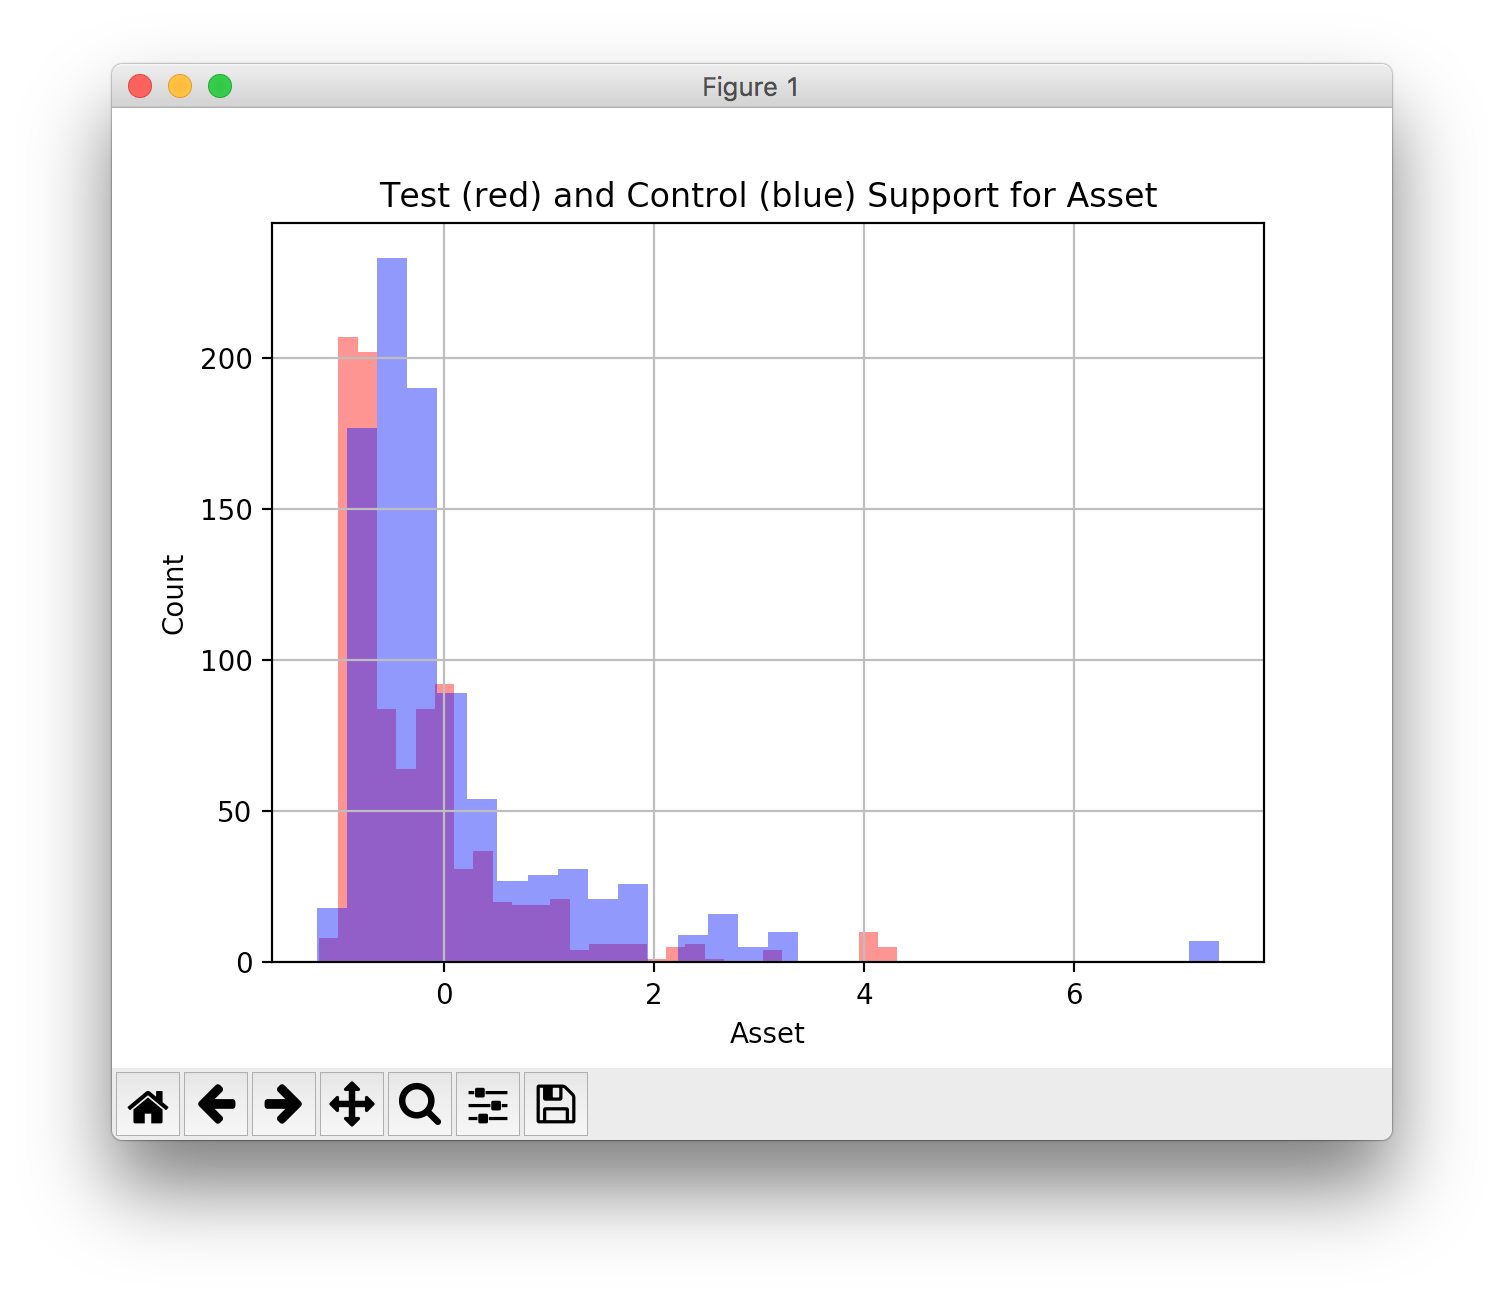
\includegraphics[width = 1.6in]{results/casual/indepDirFinlL/spx/altman/asset.png}} &
\subfigure[Cash Gen/Cash Reqd]{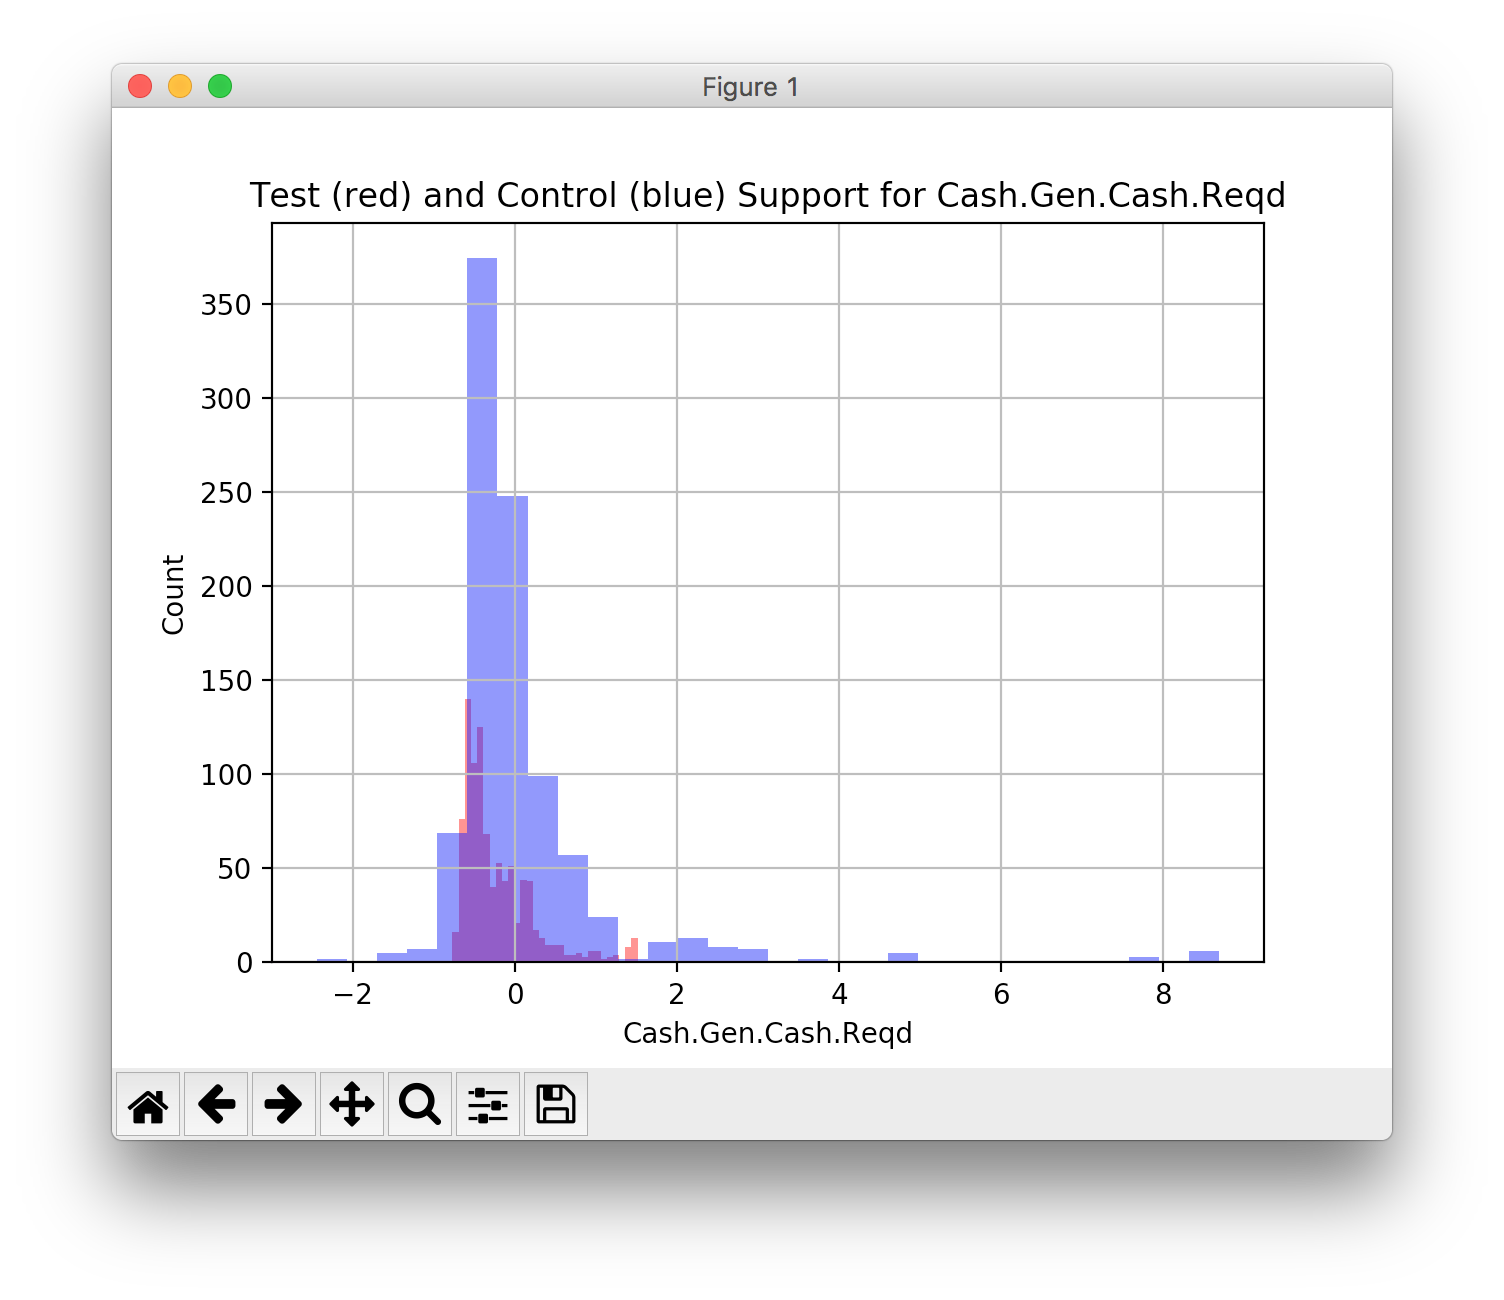
\includegraphics[width = 1.6in]{results/casual/indepDirFinlL/spx/altman/Cash_gen_cash_reqd.png}} &
\subfigure[Dvd Yld]{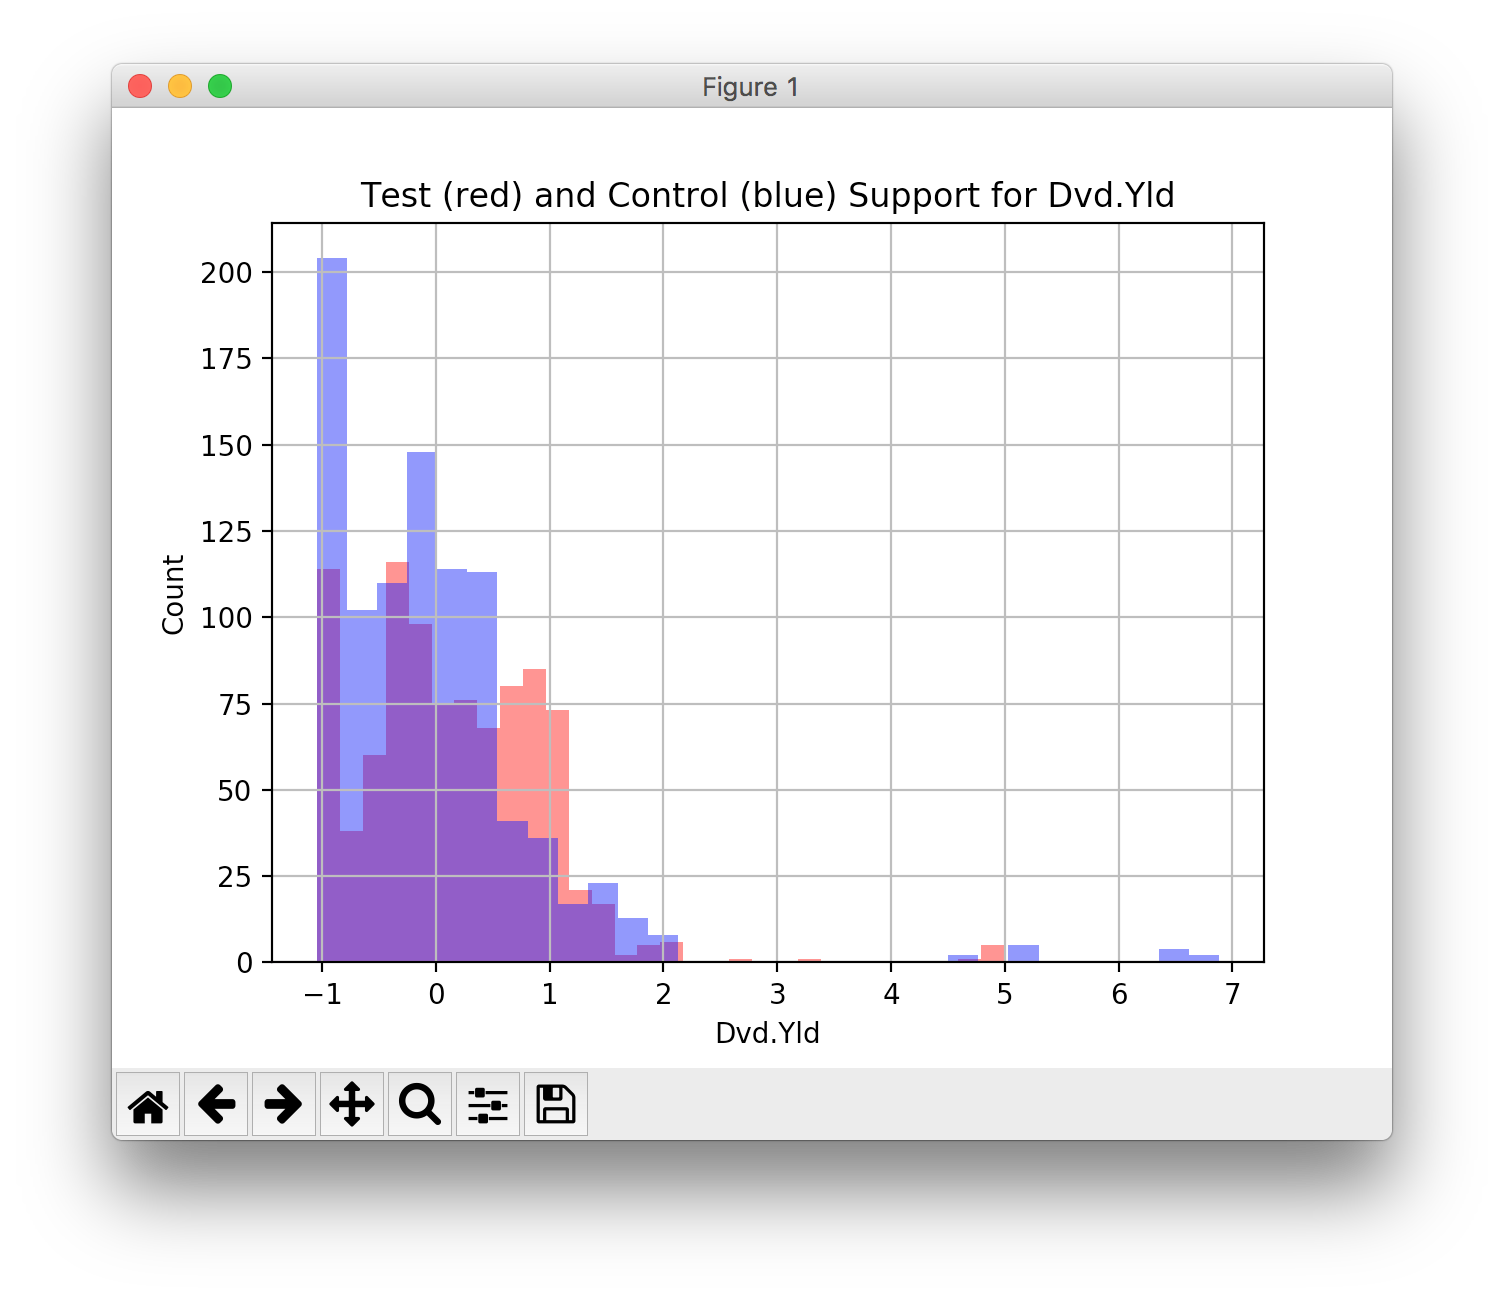
\includegraphics[width = 1.6in]{results/casual/indepDirFinlL/spx/altman/Dvd_Yld.png}} \\
\subfigure[Fin Lev]{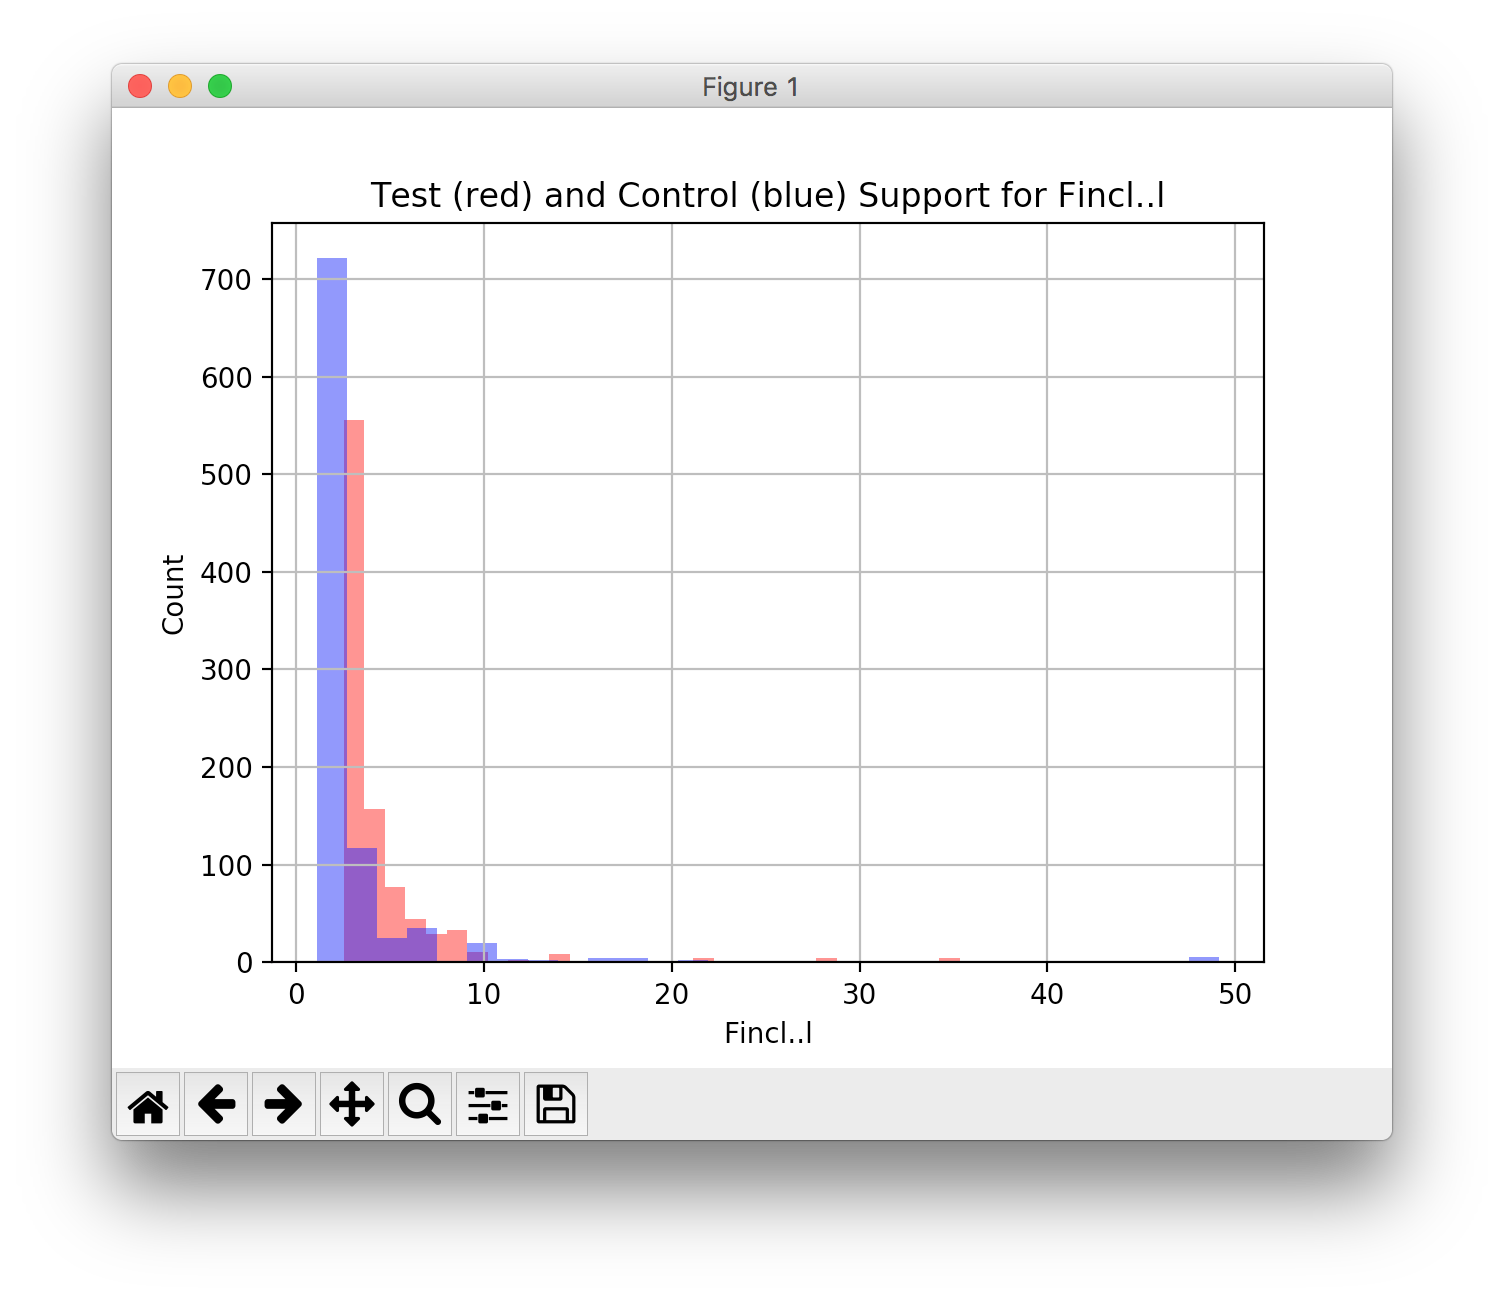
\includegraphics[width = 1.6in]{results/casual/indepDirFinlL/spx/altman/Fincl_l.png}} &
\subfigure[Net Debt/EBITDA]{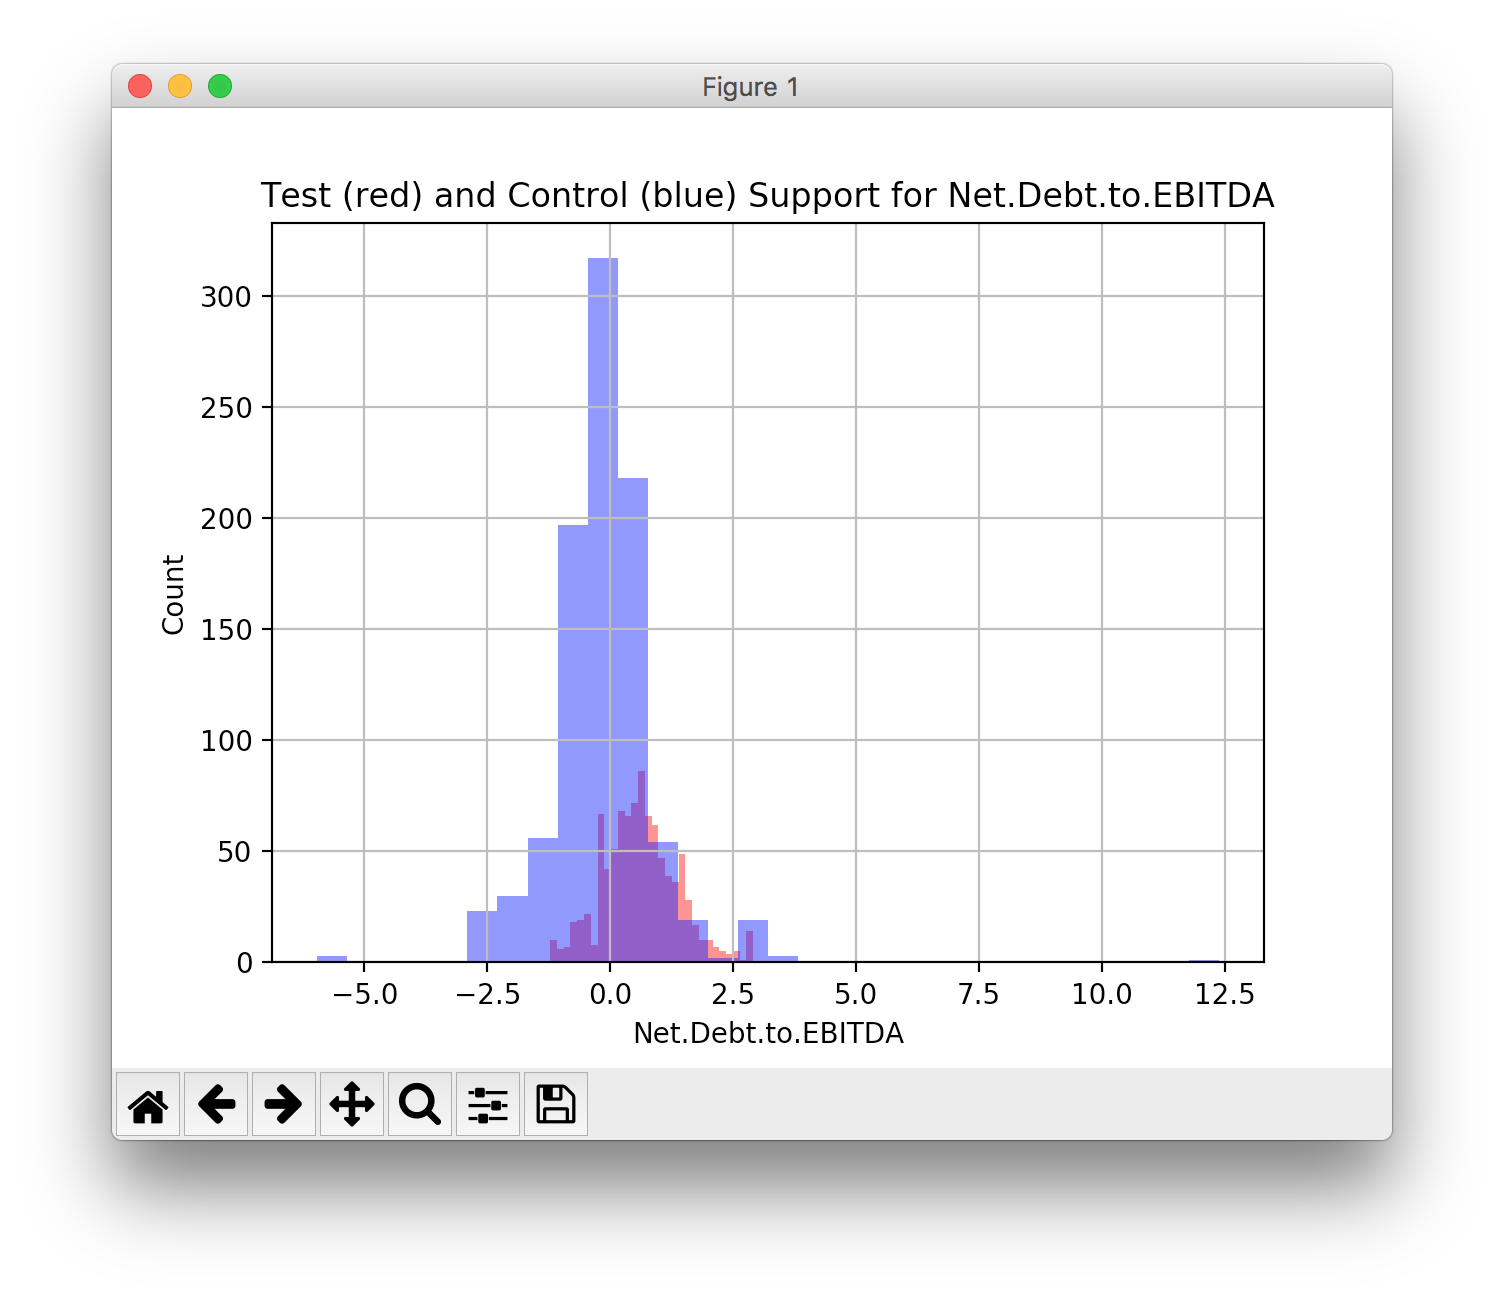
\includegraphics[width = 1.6in]{results/casual/indepDirFinlL/spx/altman/Net_dedt_to_ebitda.png}} &
\subfigure[OPM 12Mth]{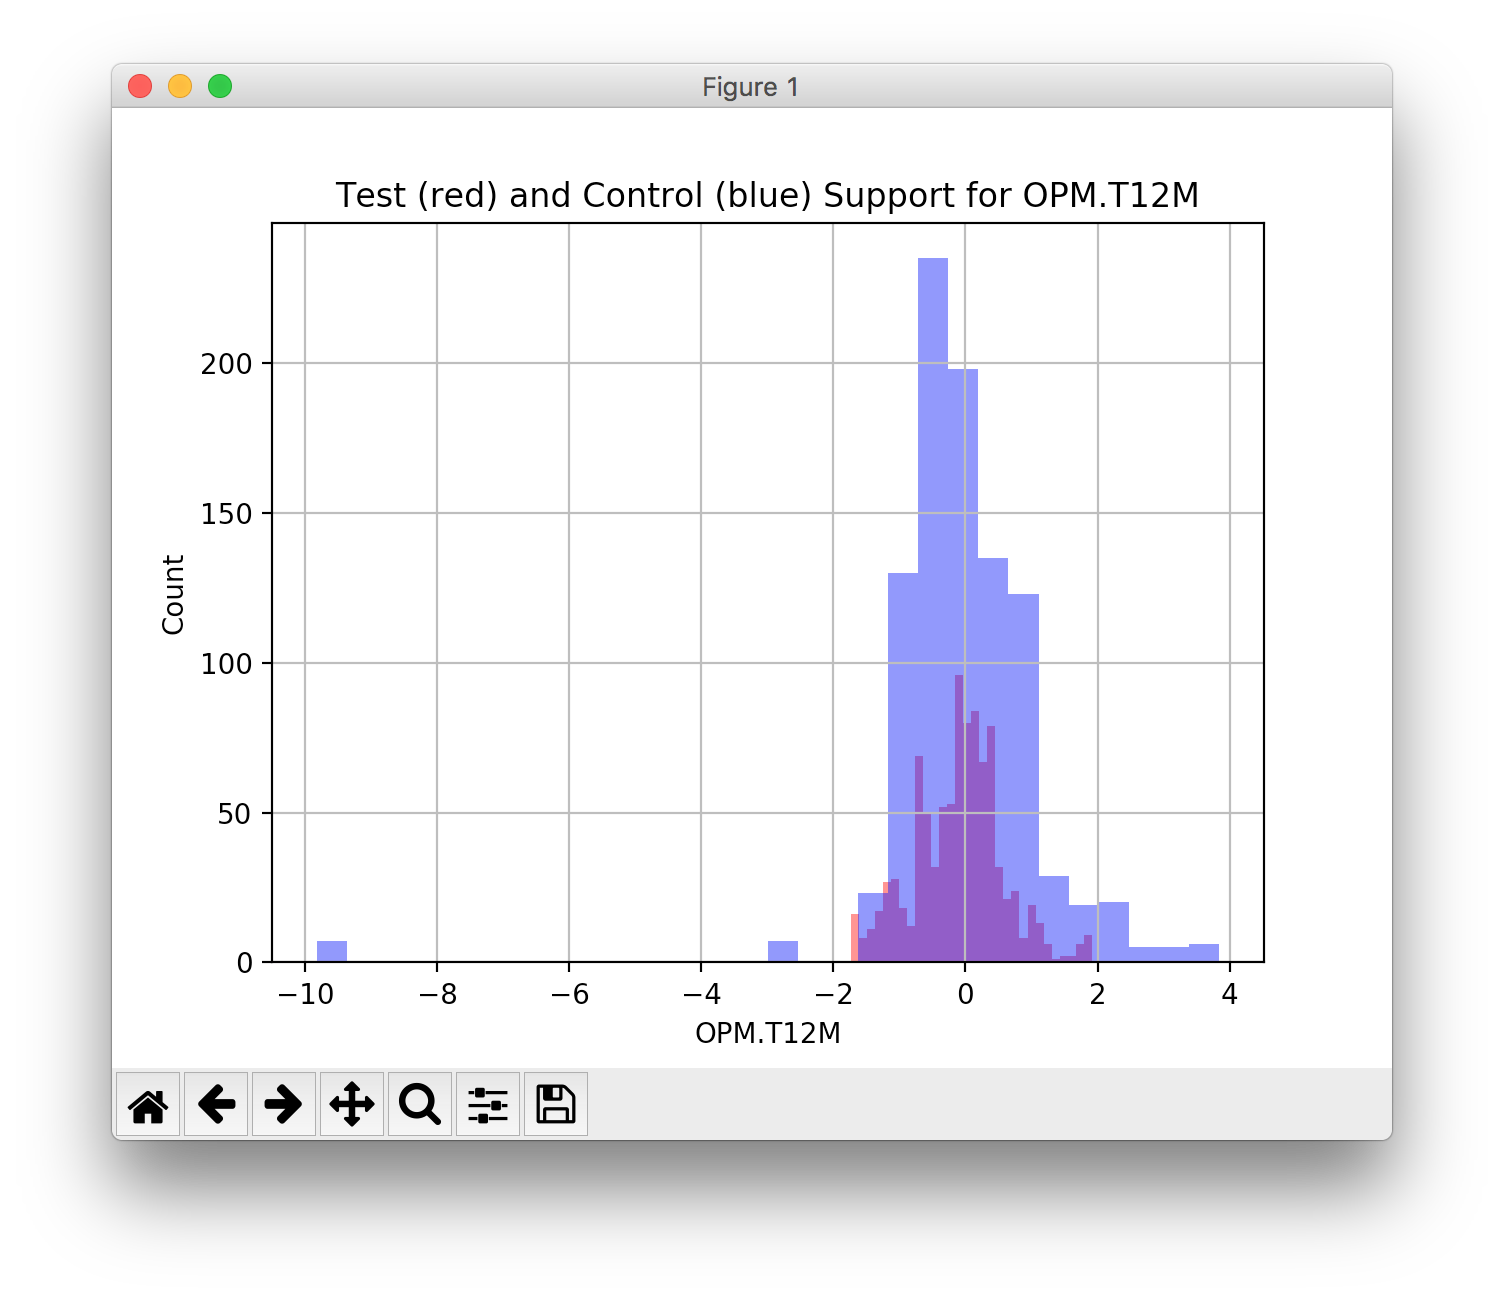
\includegraphics[width = 1.6in]{results/casual/indepDirFinlL/spx/altman/opm_t12m.png}} \\
\subfigure[P/B]{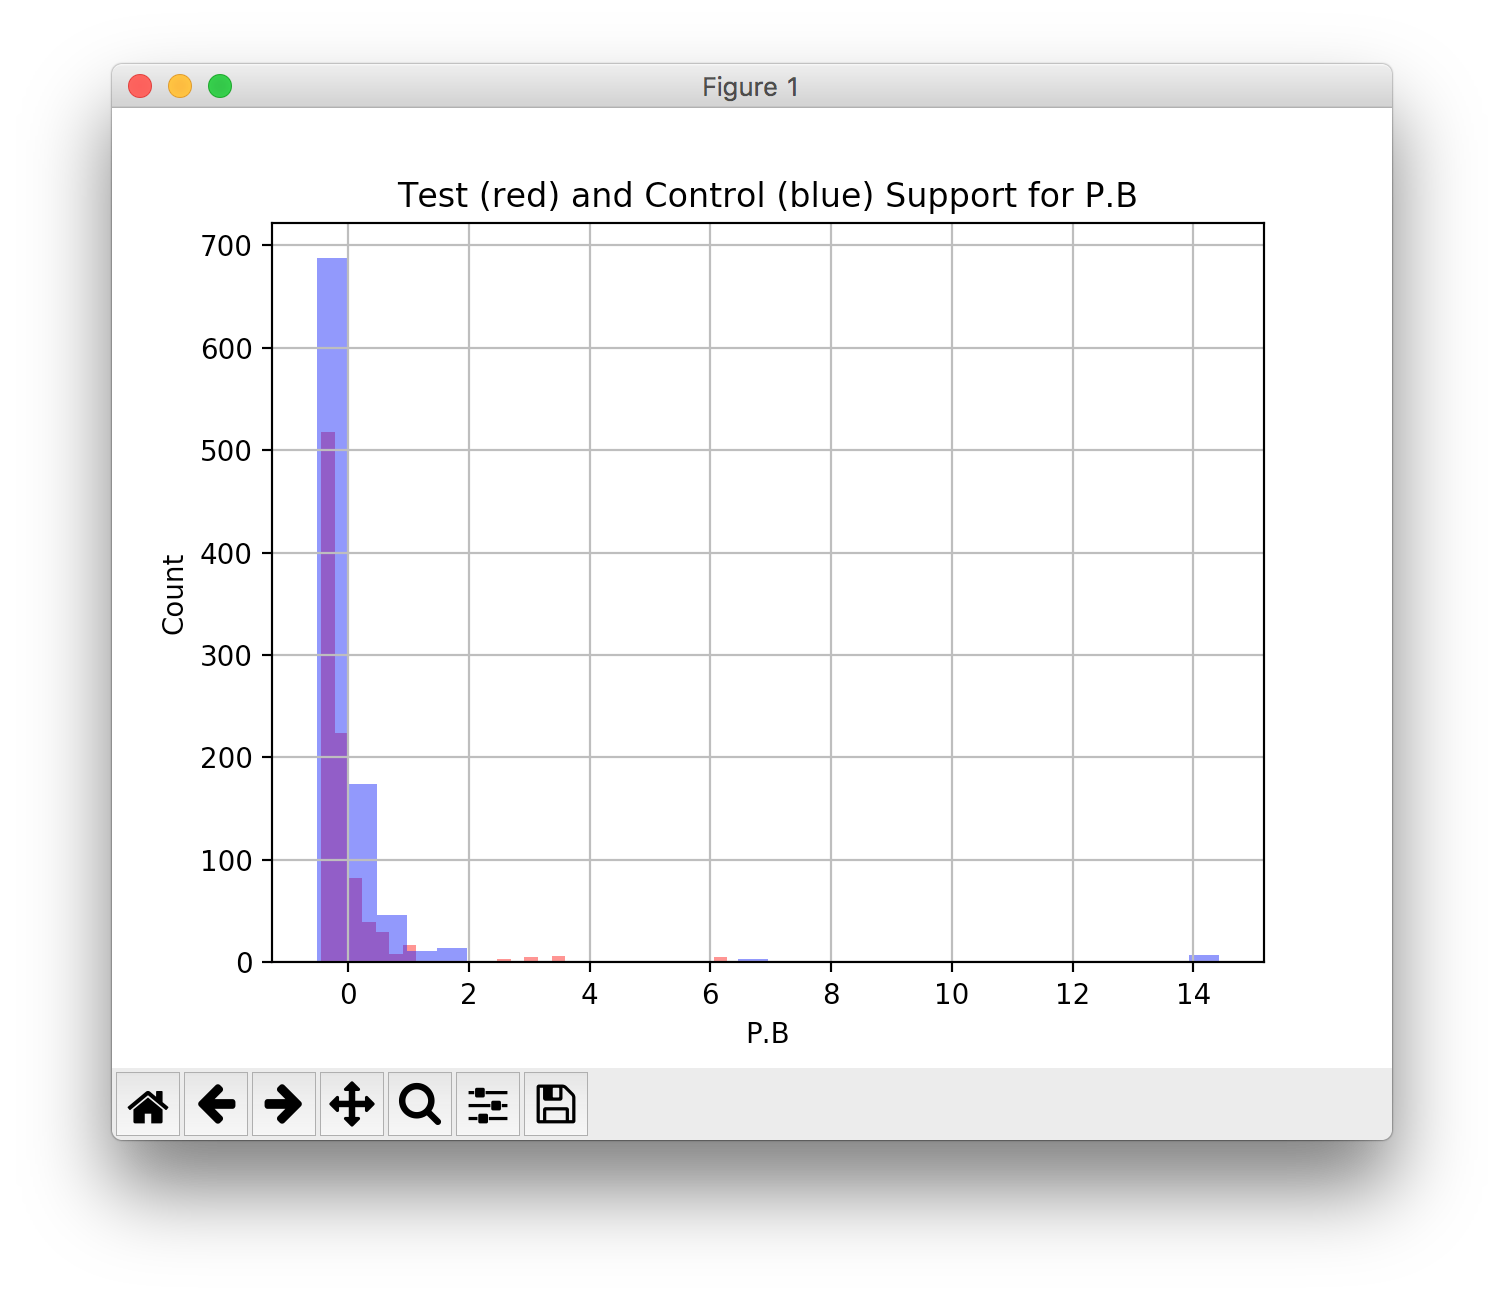
\includegraphics[width = 1.6in]{results/casual/indepDirFinlL/spx/altman/P_B.png}} &
\subfigure[P/EBITDA]{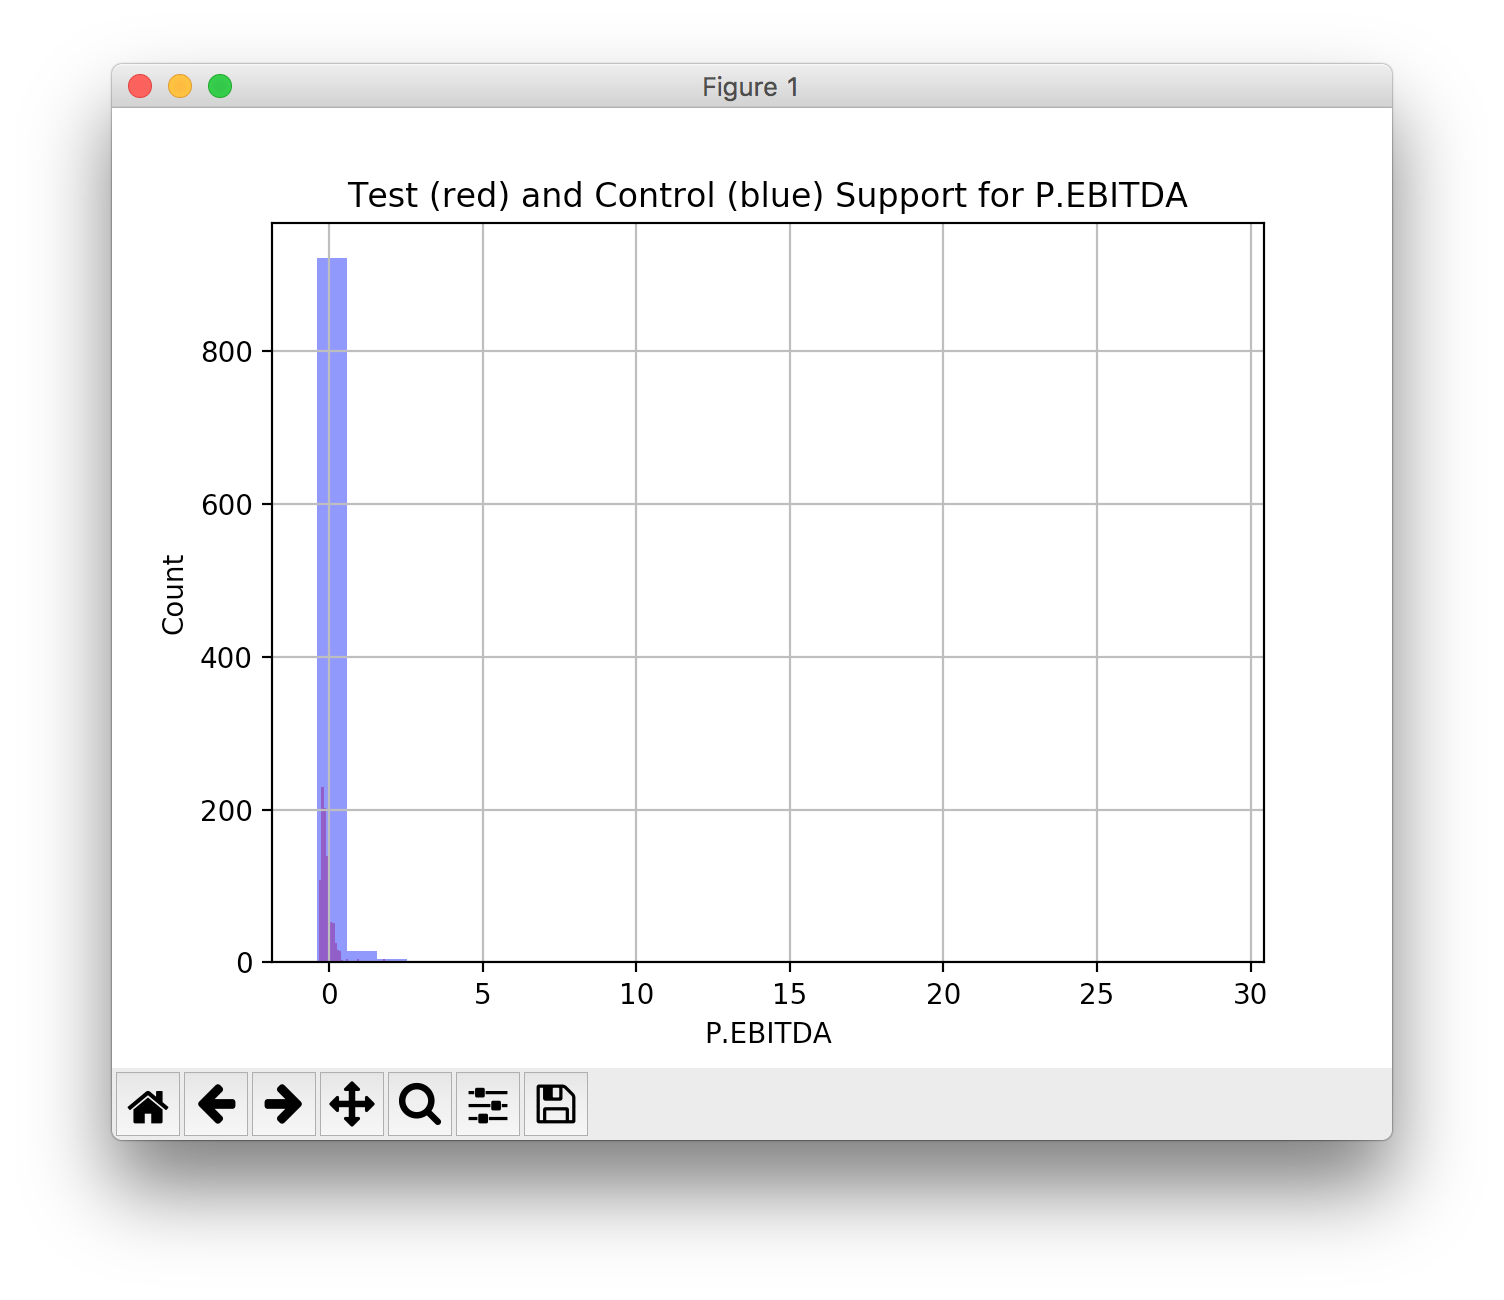
\includegraphics[width = 1.6in]{results/casual/indepDirFinlL/spx/altman/P_EBITDA.png}} &
\subfigure[Tax]{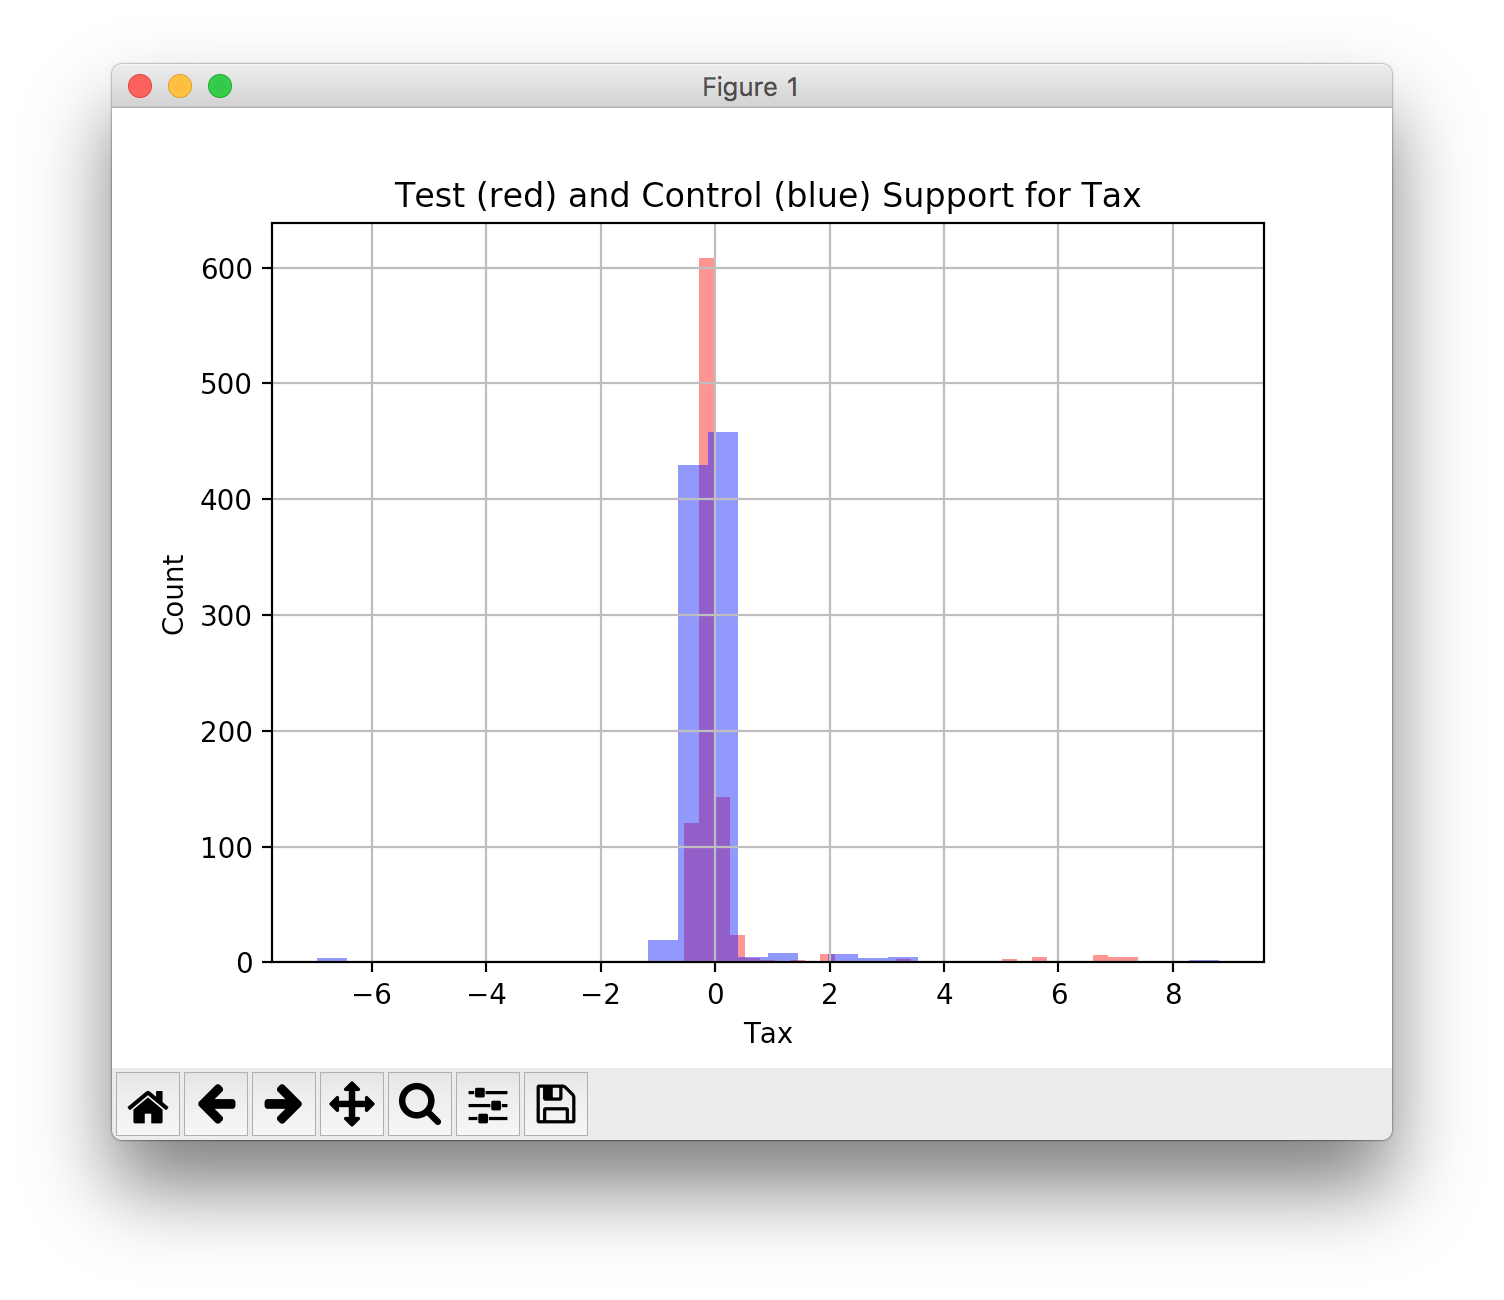
\includegraphics[width = 1.6in]{results/casual/indepDirFinlL/spx/altman/Tax.png}} \\
\end{tabular}
\caption{Causal Estimation - Independent Director \& Financial Leverage}
\end{figure}
%\fi 
\clearpage

%%%%%%%%%%%%
%%CEO Compensation
%%%%%%%%%%%%
\subsubsection{CEO Compensation}
%\iffalse
\begin{tabular}{ll}
{\bf Market} & S\&P 500  \\
{\bf Outcome} & Tobins Q Score \\
{\bf Treatment} & CEO Comp $>$ median(CEO Comp)? 1 : 0  \\
{\bf Motivating Statement} & \ref{wildOne} [agrees, original] \\
{\bf Estimate ($\% \Delta , 95\% \ CI$)} &  (-0.11, -0.085, -0.06) \\~\\
{\bf Matching Plots} &
\end{tabular}
\begin{figure}[h!]
\begin{tabular}{ccc}
\subfigure[Assets]{\includegraphics[width = 1.5in]{results/casual/CEOPayOverMedian/tobin/Asset.png}} &
\subfigure[EBITDA 12Mth]{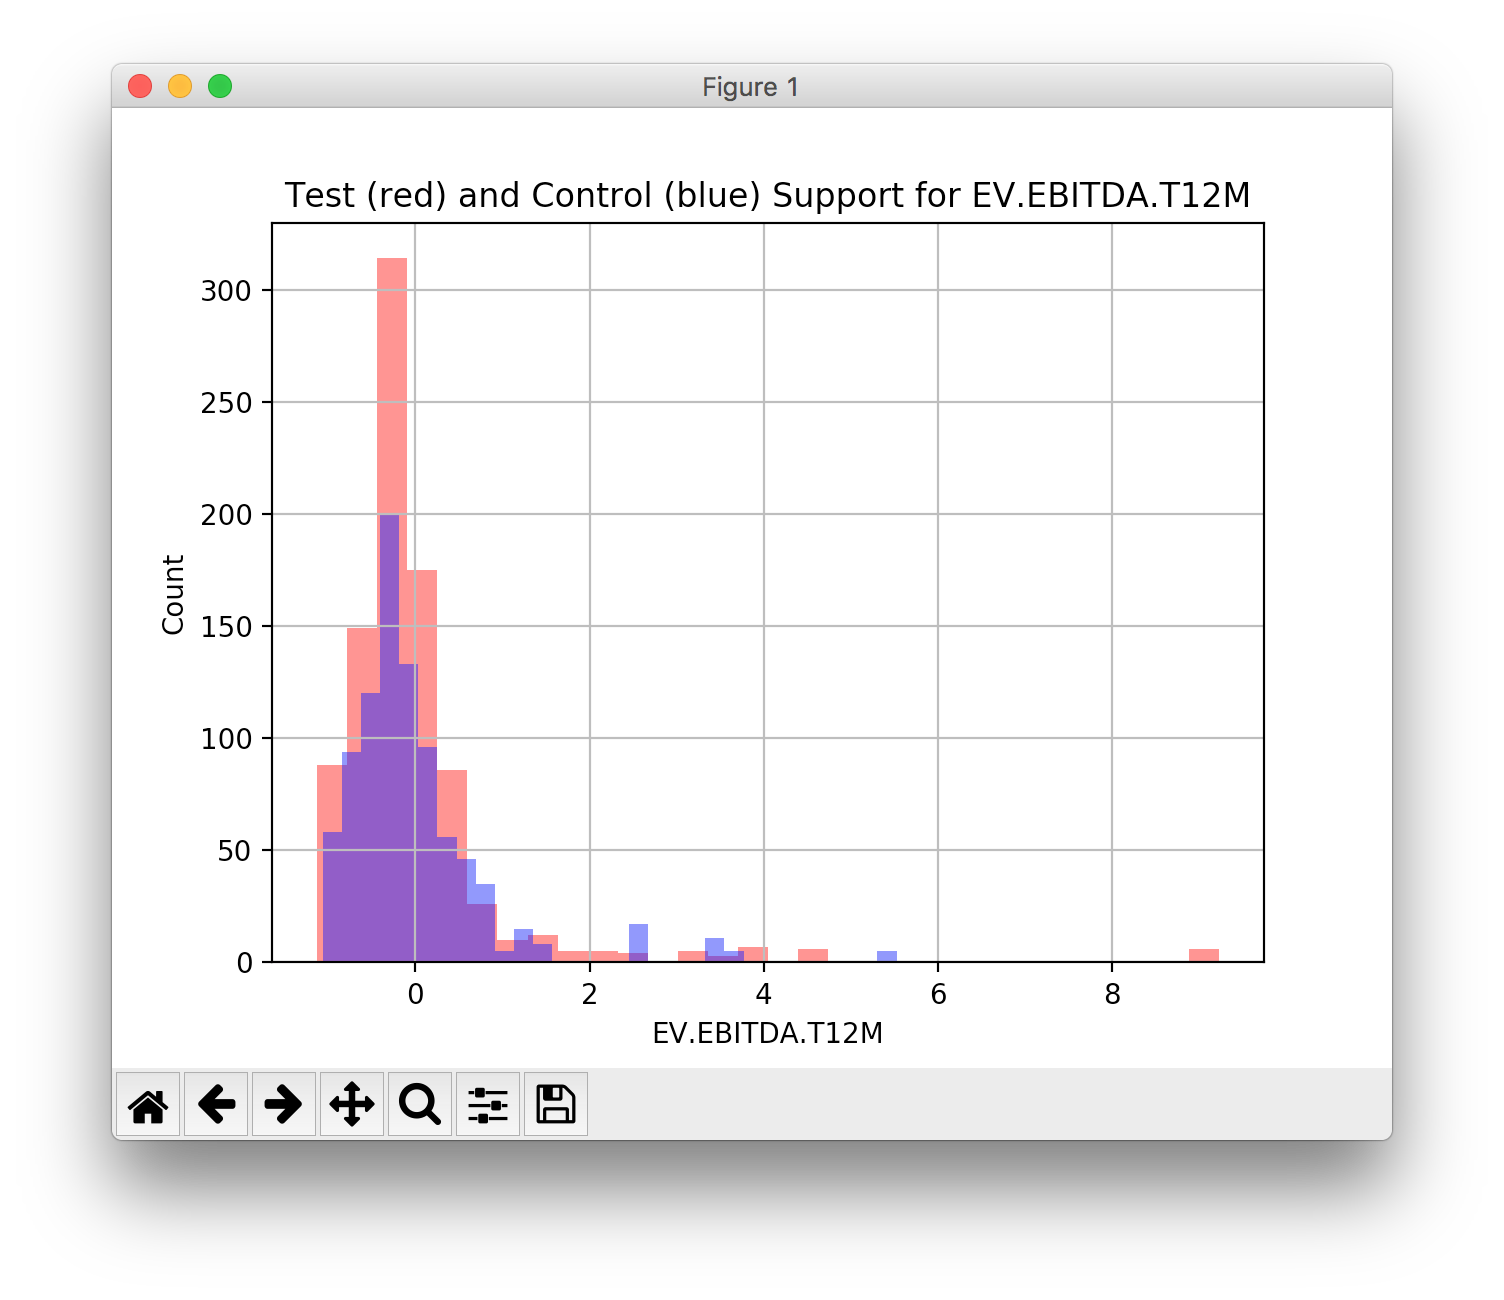
\includegraphics[width = 1.5in]{results/casual/CEOPayOverMedian/tobin/EV_EBITDA_T12M.png}} &
\subfigure[Fin Lev]{\includegraphics[width = 1.5in]{results/casual/CEOPayOverMedian/tobin/Fincl.png}} \\
\subfigure[Net Debt/EBITDA]{\includegraphics[width = 1.5in]{results/casual/CEOPayOverMedian/tobin/Net_Debt_to_EBITDA.png}} &
\subfigure[Norm NI to NI for Cmn]{\includegraphics[width = 1.5in]{results/casual/CEOPayOverMedian/tobin/Norm_NI_to_NI_for_Cmn.png}} &
\subfigure[OPM 12Mth]{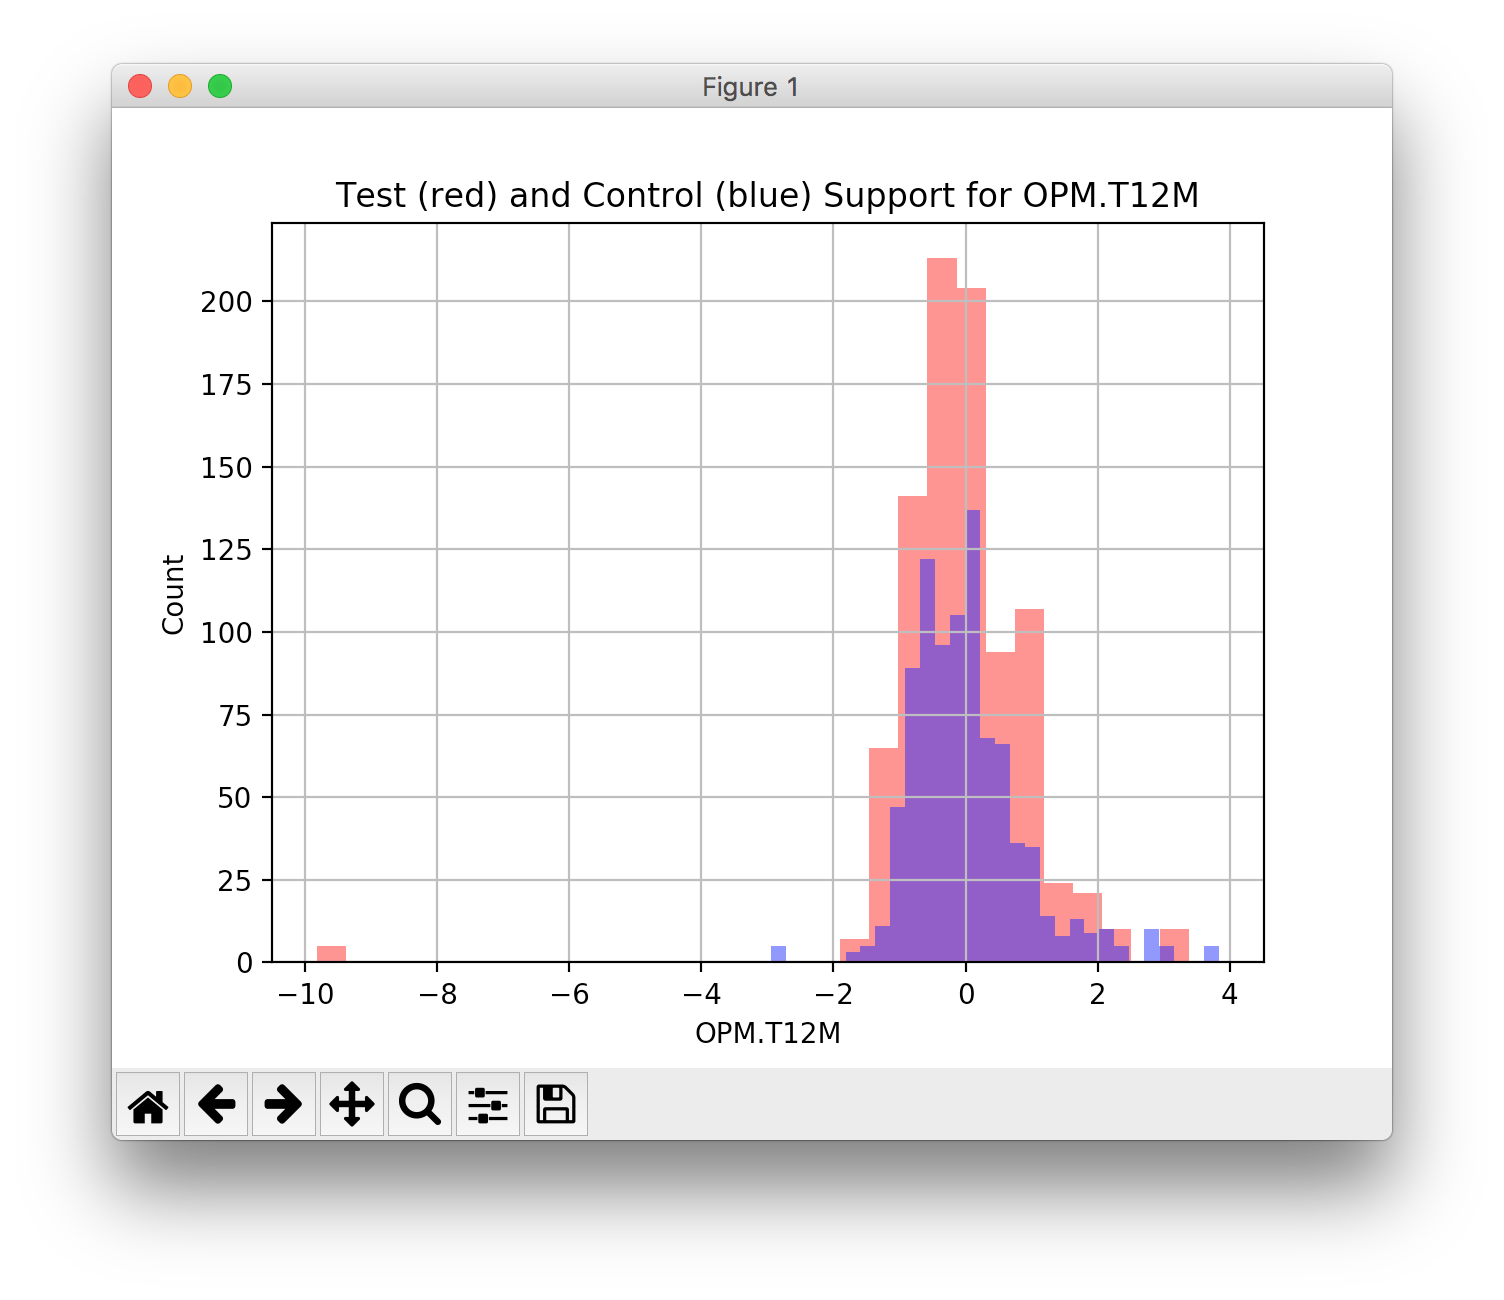
\includegraphics[width = 1.5in]{results/casual/CEOPayOverMedian/tobin/OPM_T12M.png}} \\
\subfigure[P/B]{\includegraphics[width = 1.5in]{results/casual/CEOPayOverMedian/tobin/P_B.png}}  &
%\subfigure[P/EBITDA]{\includegraphics[width = 1.5in]{results/casual/CEOPayOverMedian/tobin/P_EBITDA.png}}  &
\subfigure[ROC]{\includegraphics[width = 1.5in]{results/casual/CEOPayOverMedian/tobin/ROC.png}} &
\subfigure[\% Female Executives]{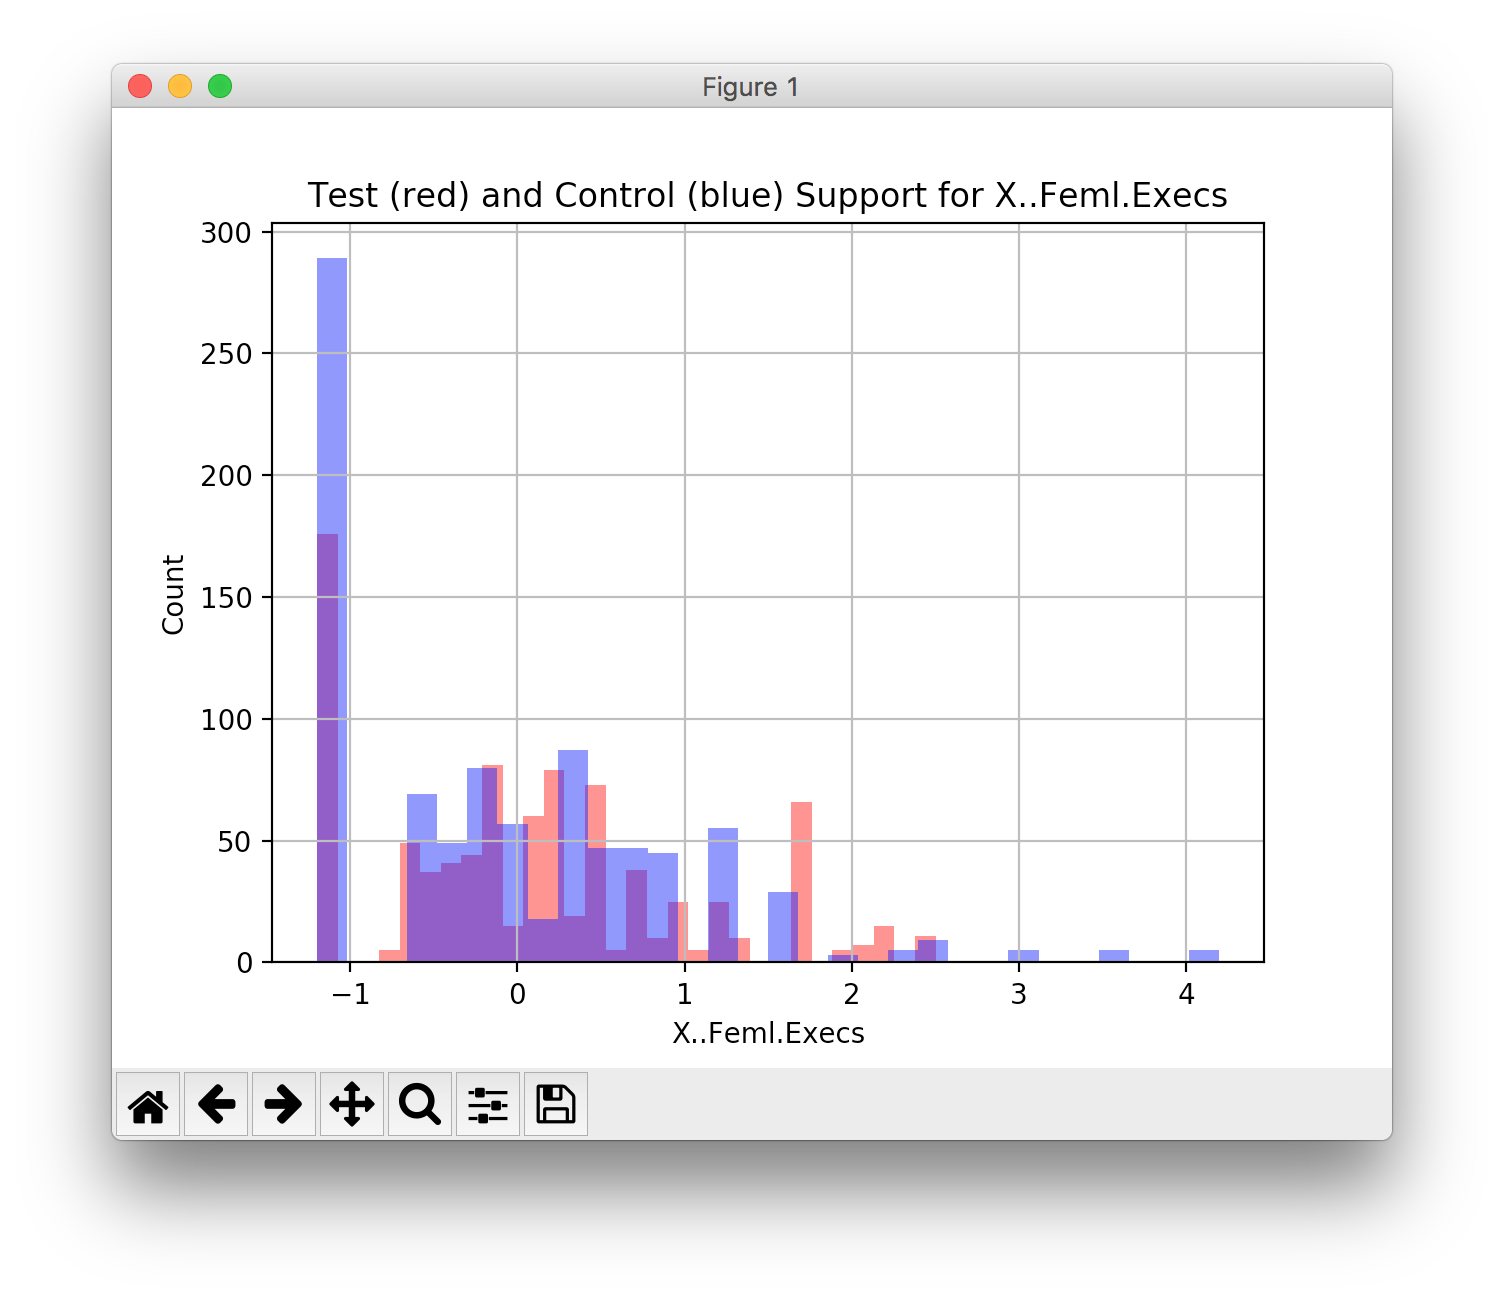
\includegraphics[width = 1.5in]{results/casual/CEOPayOverMedian/tobin/X_Feml_Execs.png}}  
\end{tabular}
\caption{Causal Estimation - CEO Compensation}
\end{figure}
%\begin{figure}[h!]
%\begin{tabular}{ccc}
%\subfigure[caption]{\includegraphics[width = 1.5in]{results/casual/CEOPayOverMedian/altman/Asset.png}} &
%\subfigure[caption]{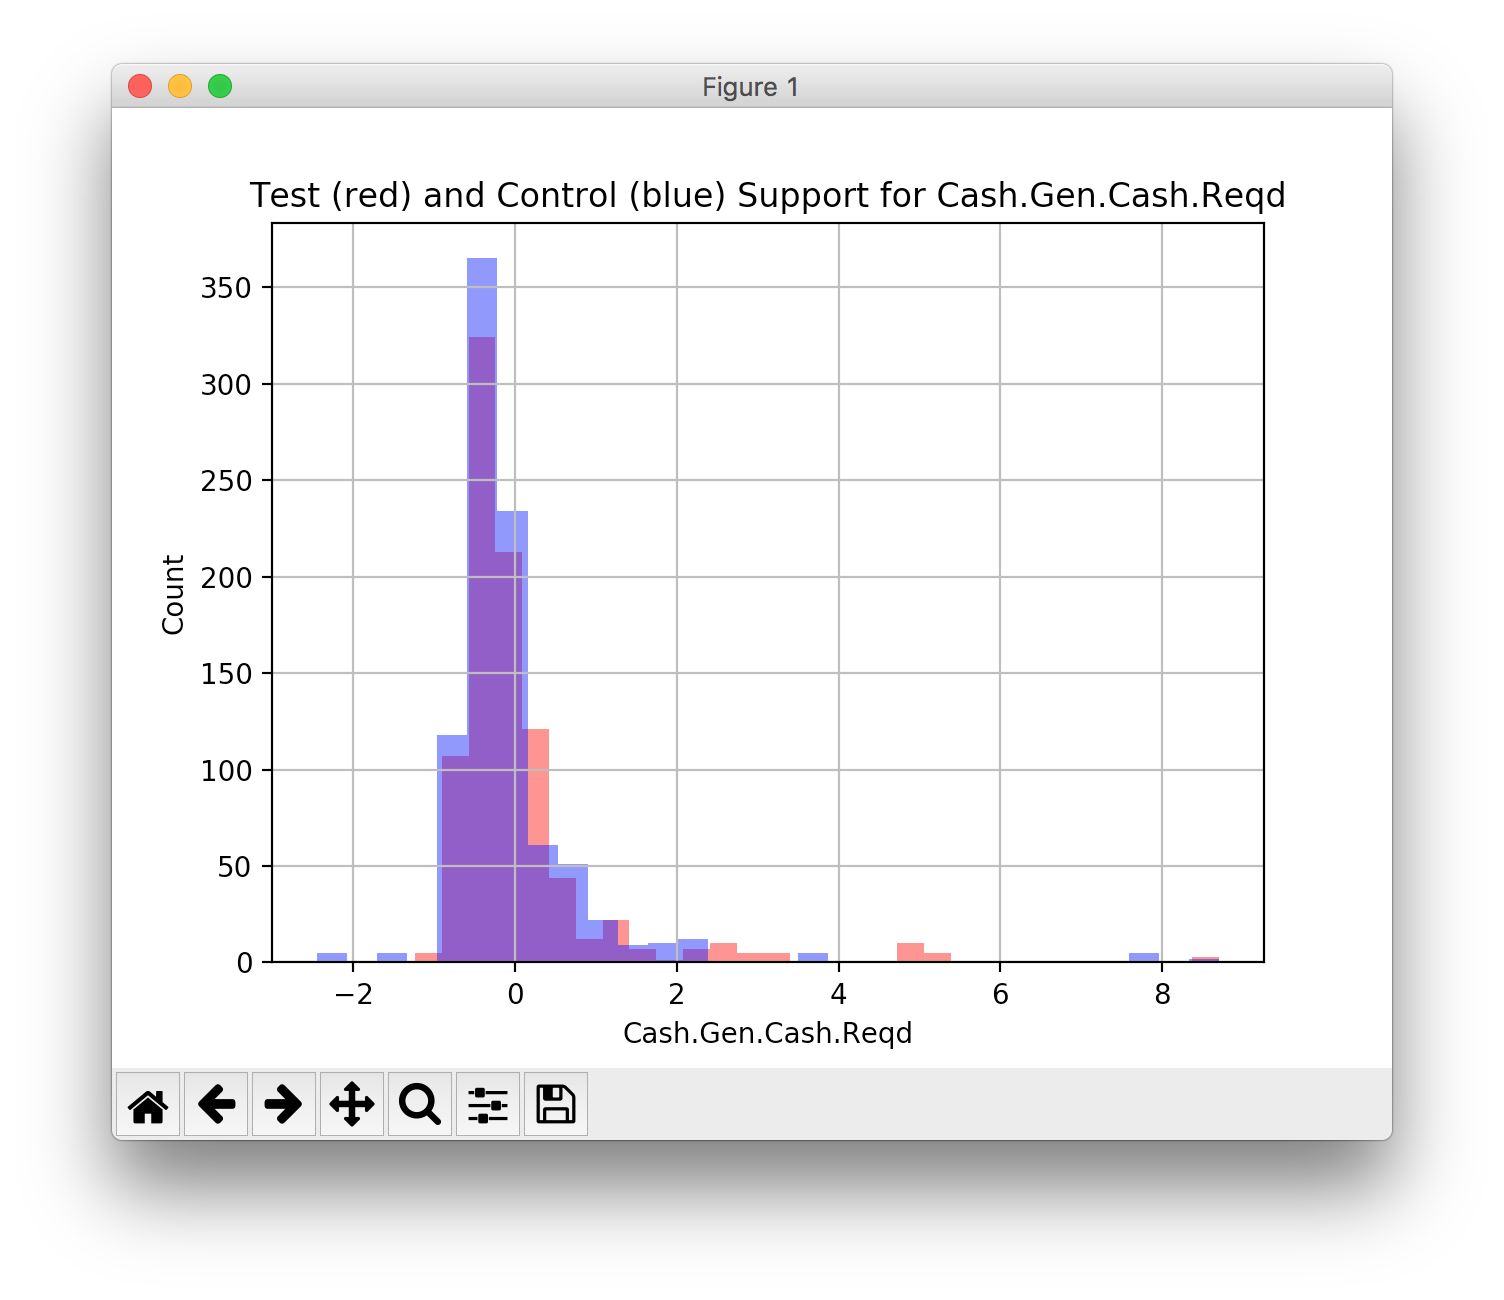
\includegraphics[width = 1.5in]{results/casual/CEOPayOverMedian/altman/Cash_Gen_Cash_Reqd.png}} &
%\subfigure[caption]{\includegraphics[width = 1.5in]{results/casual/CEOPayOverMedian/altman/Fincl.png}} \\
%\subfigure[caption]{\includegraphics[width = 1.5in]{results/casual/CEOPayOverMedian/altman/Net_Debt_to_EBITDA.png}} &
%\subfigure[caption]{\includegraphics[width = 1.5in]{results/casual/CEOPayOverMedian/altman/Norm_NI_to_NI_for_Cmn.png}} &
%\subfigure[caption]{\includegraphics[width = 1.5in]{results/casual/CEOPayOverMedian/altman/P_B.png}} \\
%\subfigure[caption]{\includegraphics[width = 1.5in]{results/casual/CEOPayOverMedian/altman/P_EBITDA.png}}  &
%\subfigure[caption]{\includegraphics[width = 1.5in]{results/casual/CEOPayOverMedian/altman/ROC.png}}  &
%\subfigure[caption]{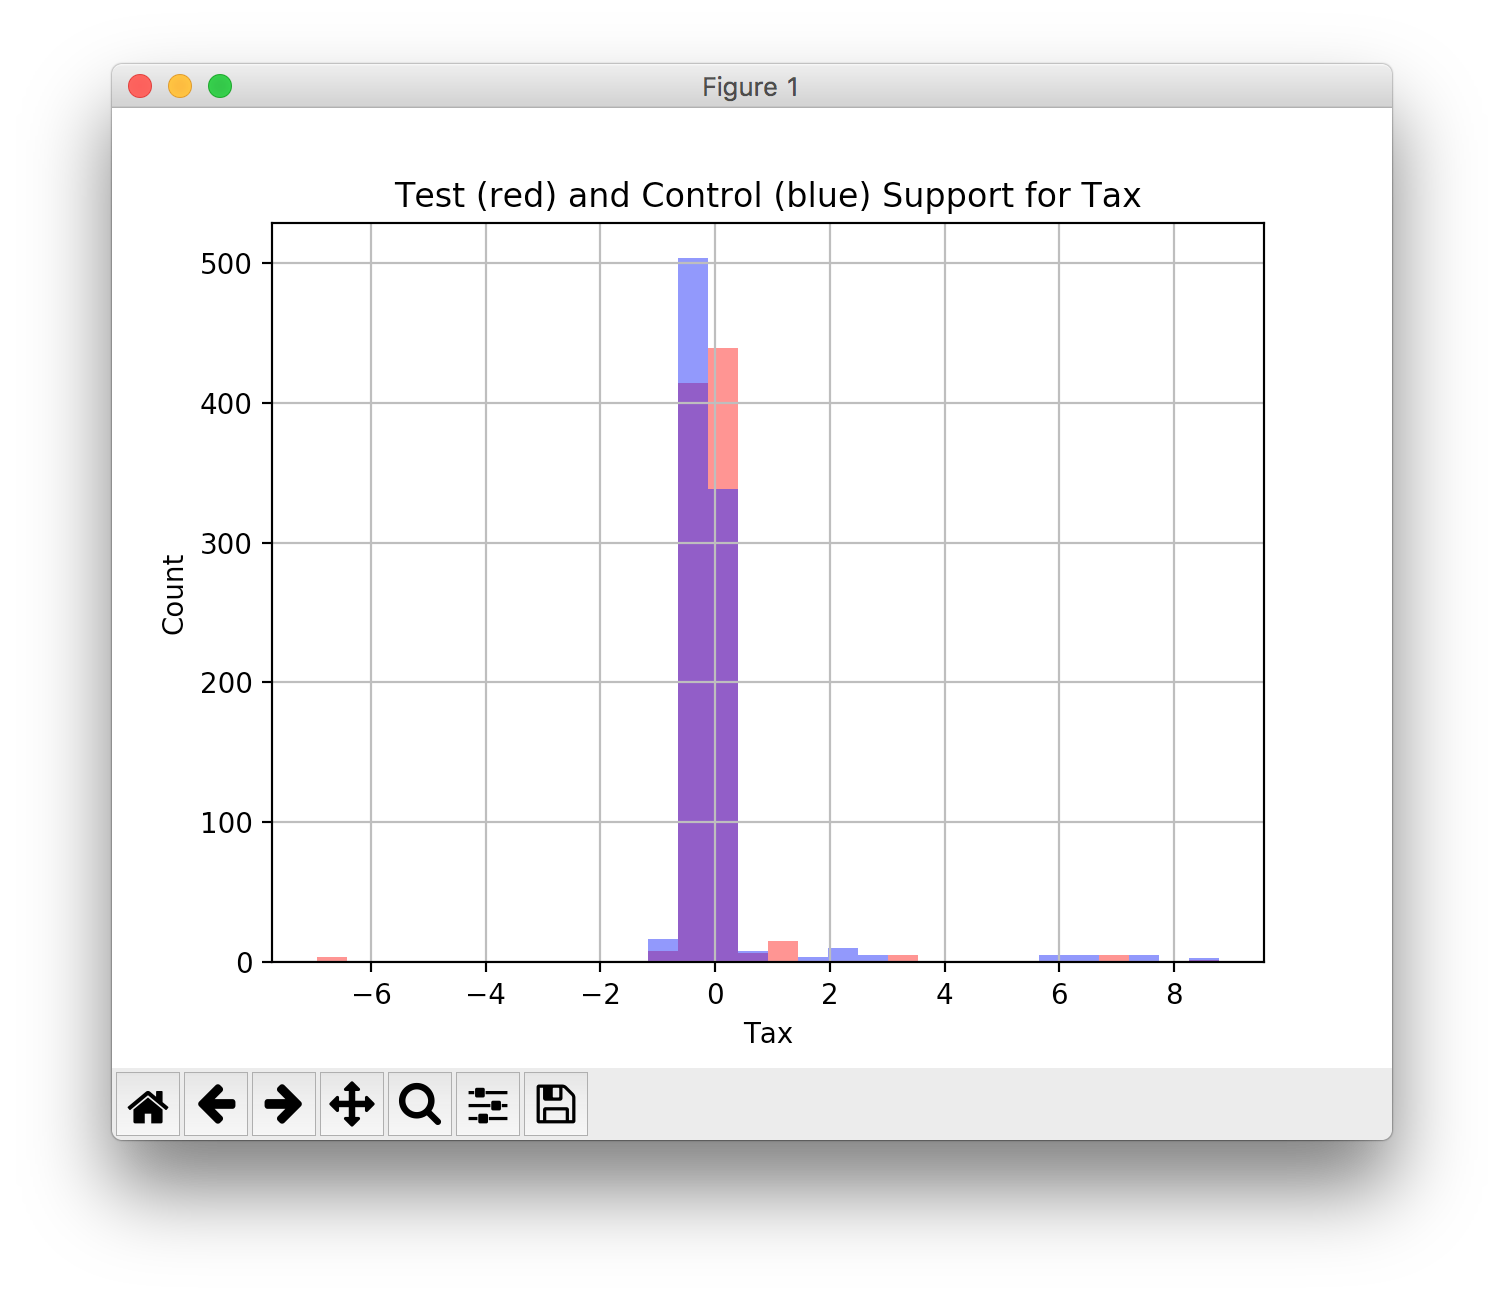
\includegraphics[width = 1.5in]{results/casual/CEOPayOverMedian/altman/Tax.png}} \\
%\subfigure[caption]{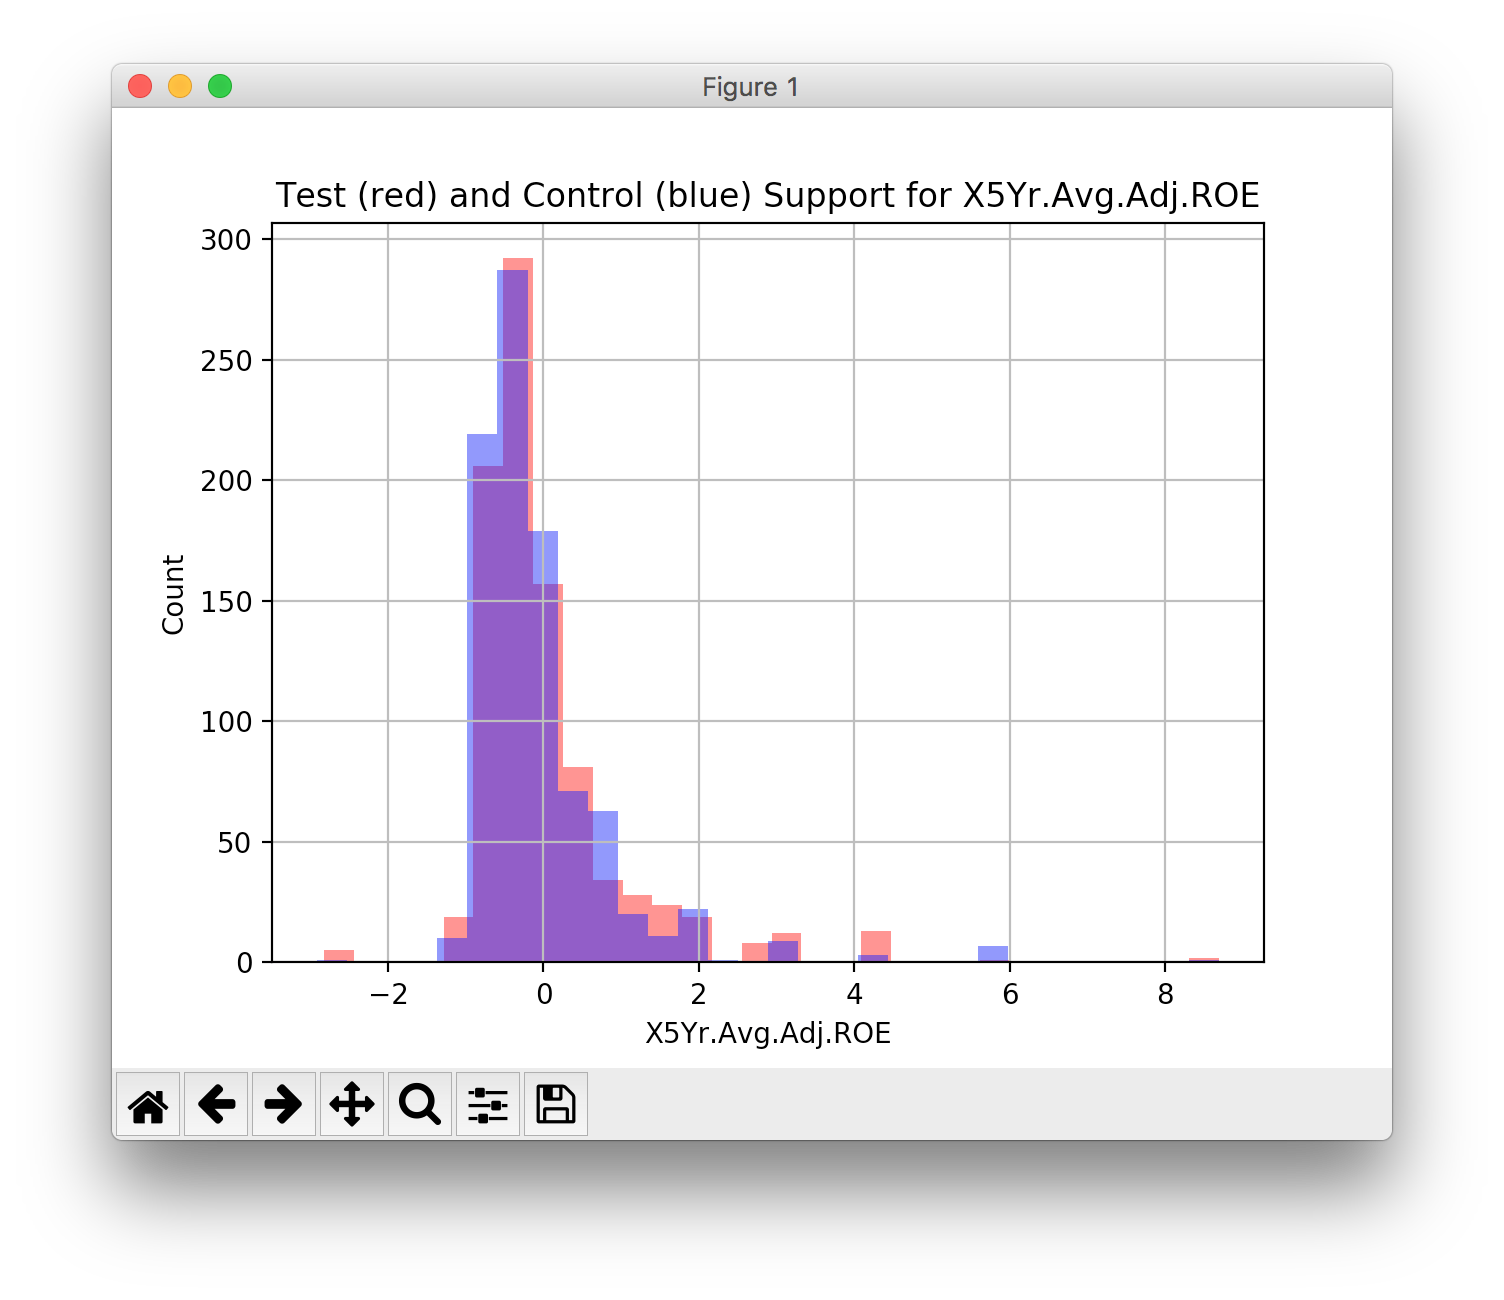
\includegraphics[width = 1.5in]{results/casual/CEOPayOverMedian/altman/X5Yr_Avg_Adj_ROE.png}}  
%\end{tabular}
%\caption{CEOPayOverMedian / Altman Z}
%\end{figure}
%{\bf Interval: } {(-0.055123647006892637, -0.03307470810522401, -0.0064863255004465239)}
%\fi
\clearpage

%%%%%%%%%%%%
%%Board of Directors Average Age
%%%%%%%%%%%%
\subsubsection{Board of Directors Average Age}
%\iffalse
\begin{tabular}{ll}
{\bf Market} & S\&P 500  \\
{\bf Outcome} & Tobins Q Score \\
{\bf Treatment} & B.O.D Avg Age $<$ mean(B.O.D Avg Age)? 1 : 0  \\
{\bf Motivating Statement} & \ref{eastOne} [disagrees, not original]   \\
{\bf Estimate ($\% \Delta , 95\% \ CI$)} &  (-0.10, -0.08 , -0.06) \\~\\
{\bf Matching Plots} &
\end{tabular}
\begin{figure}[h!]
\begin{tabular}{ccc}
\subfigure[Asset]{\includegraphics[width = 1.6in]{results/casual/BOD_Age_Rng/spx/tobin/Asset.png}} &
\subfigure[EBITDA 12Mth]{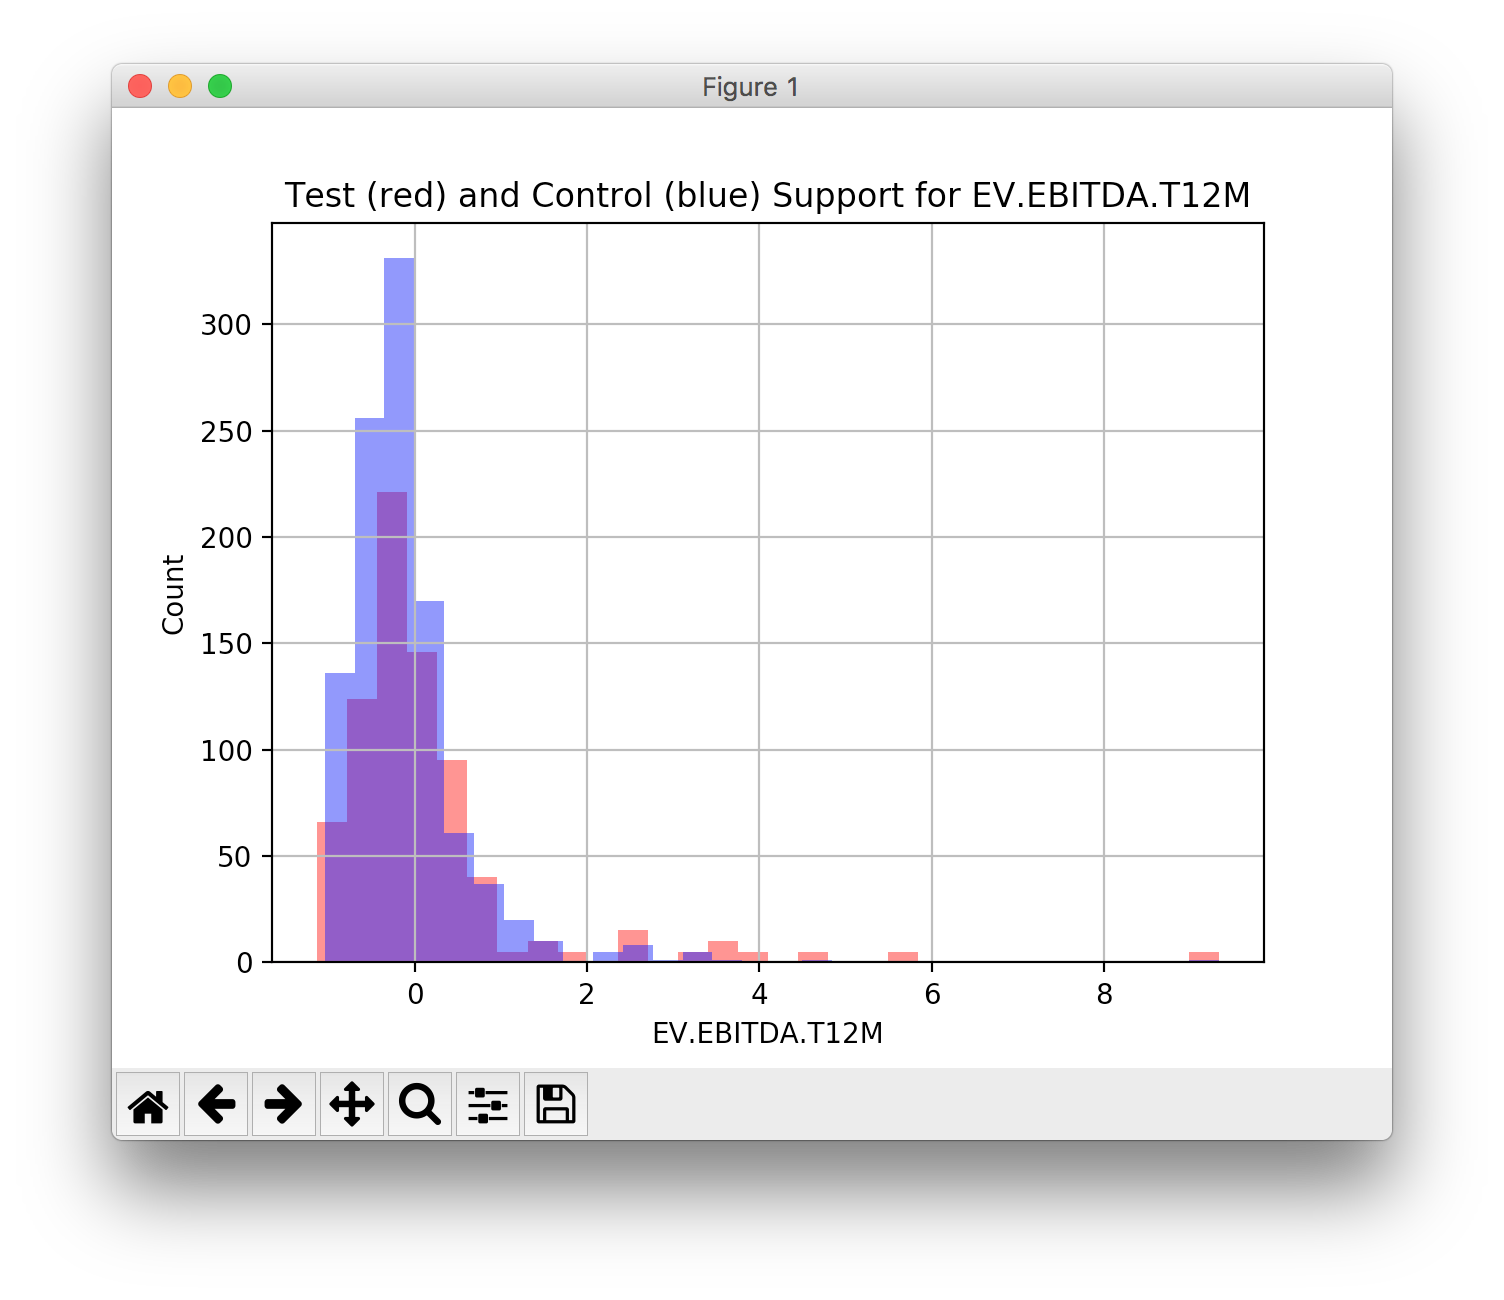
\includegraphics[width = 1.6in]{results/casual/BOD_Age_Rng/spx/tobin/EV_EBITDA_T12M.png}} &
\subfigure[Fin Lev]{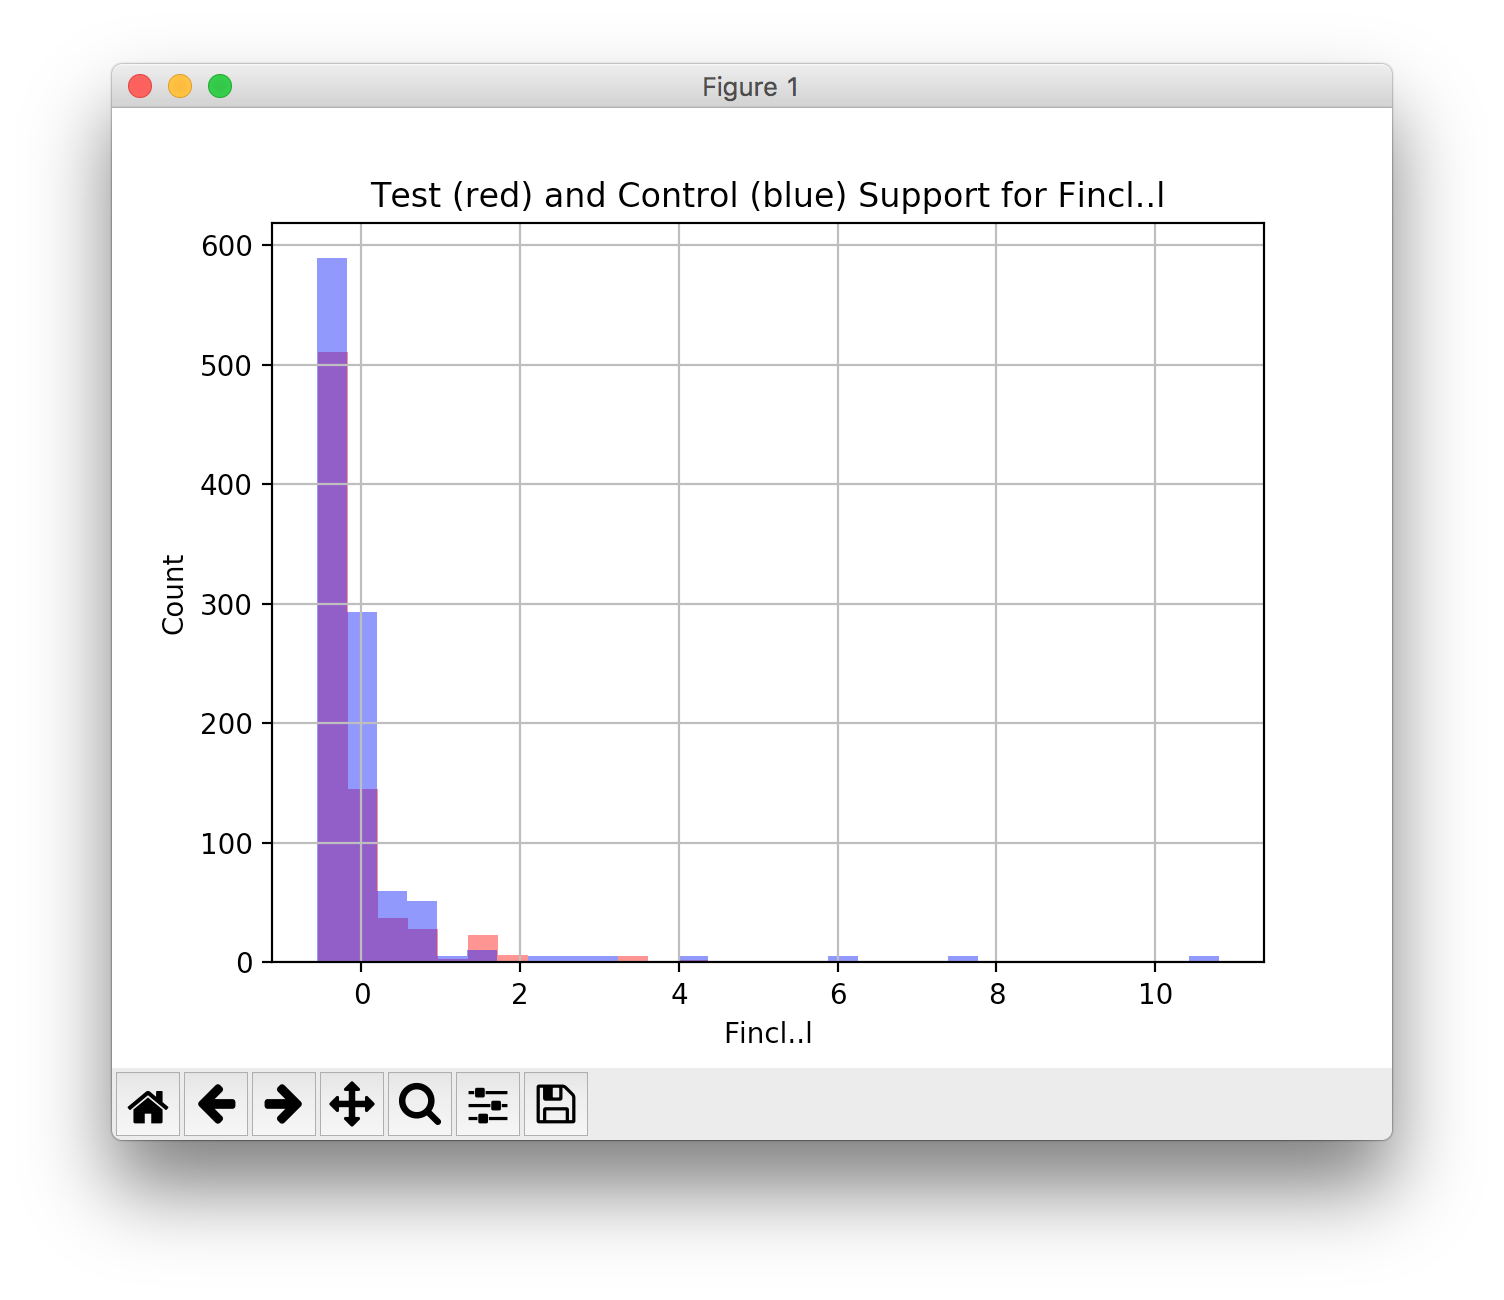
\includegraphics[width = 1.6in]{results/casual/BOD_Age_Rng/spx/tobin/Fincl.png}} \\
\subfigure[OPM 12Mth]{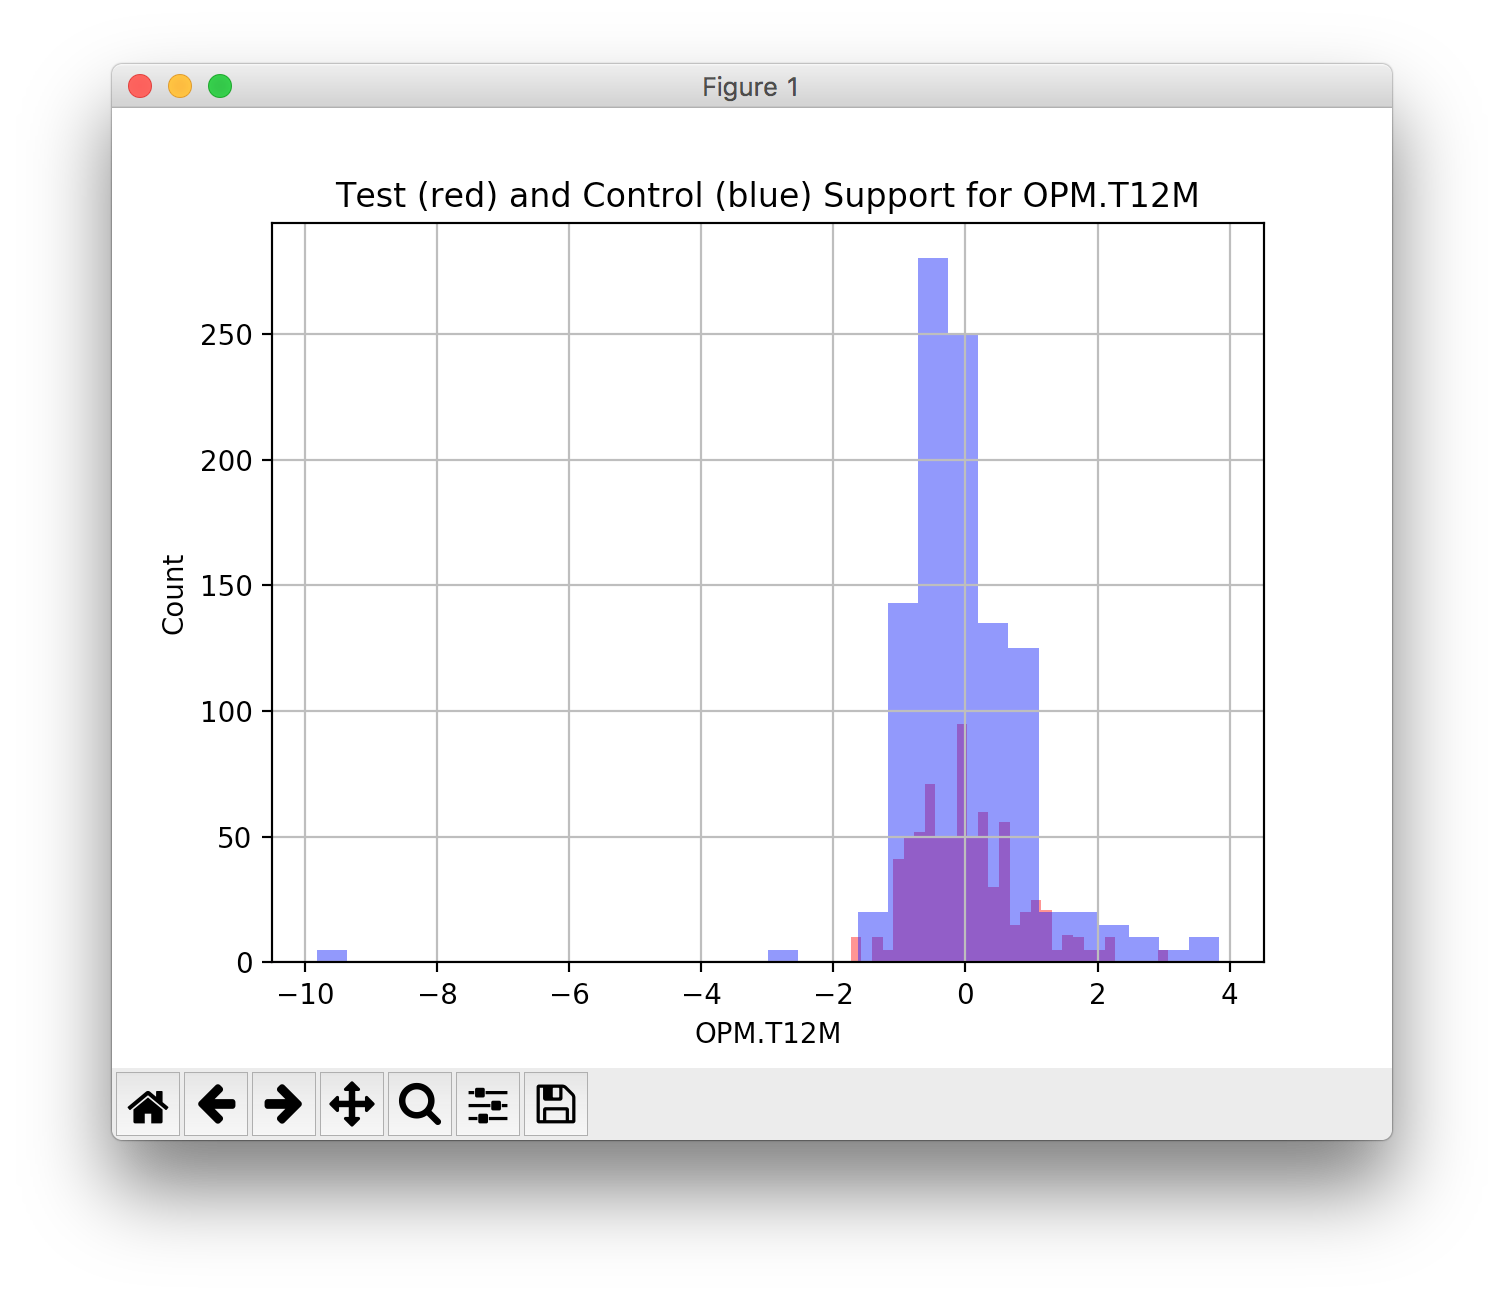
\includegraphics[width = 1.6in]{results/casual/BOD_Age_Rng/spx/tobin/OPM_T12M.png}} &
\subfigure[P/B]{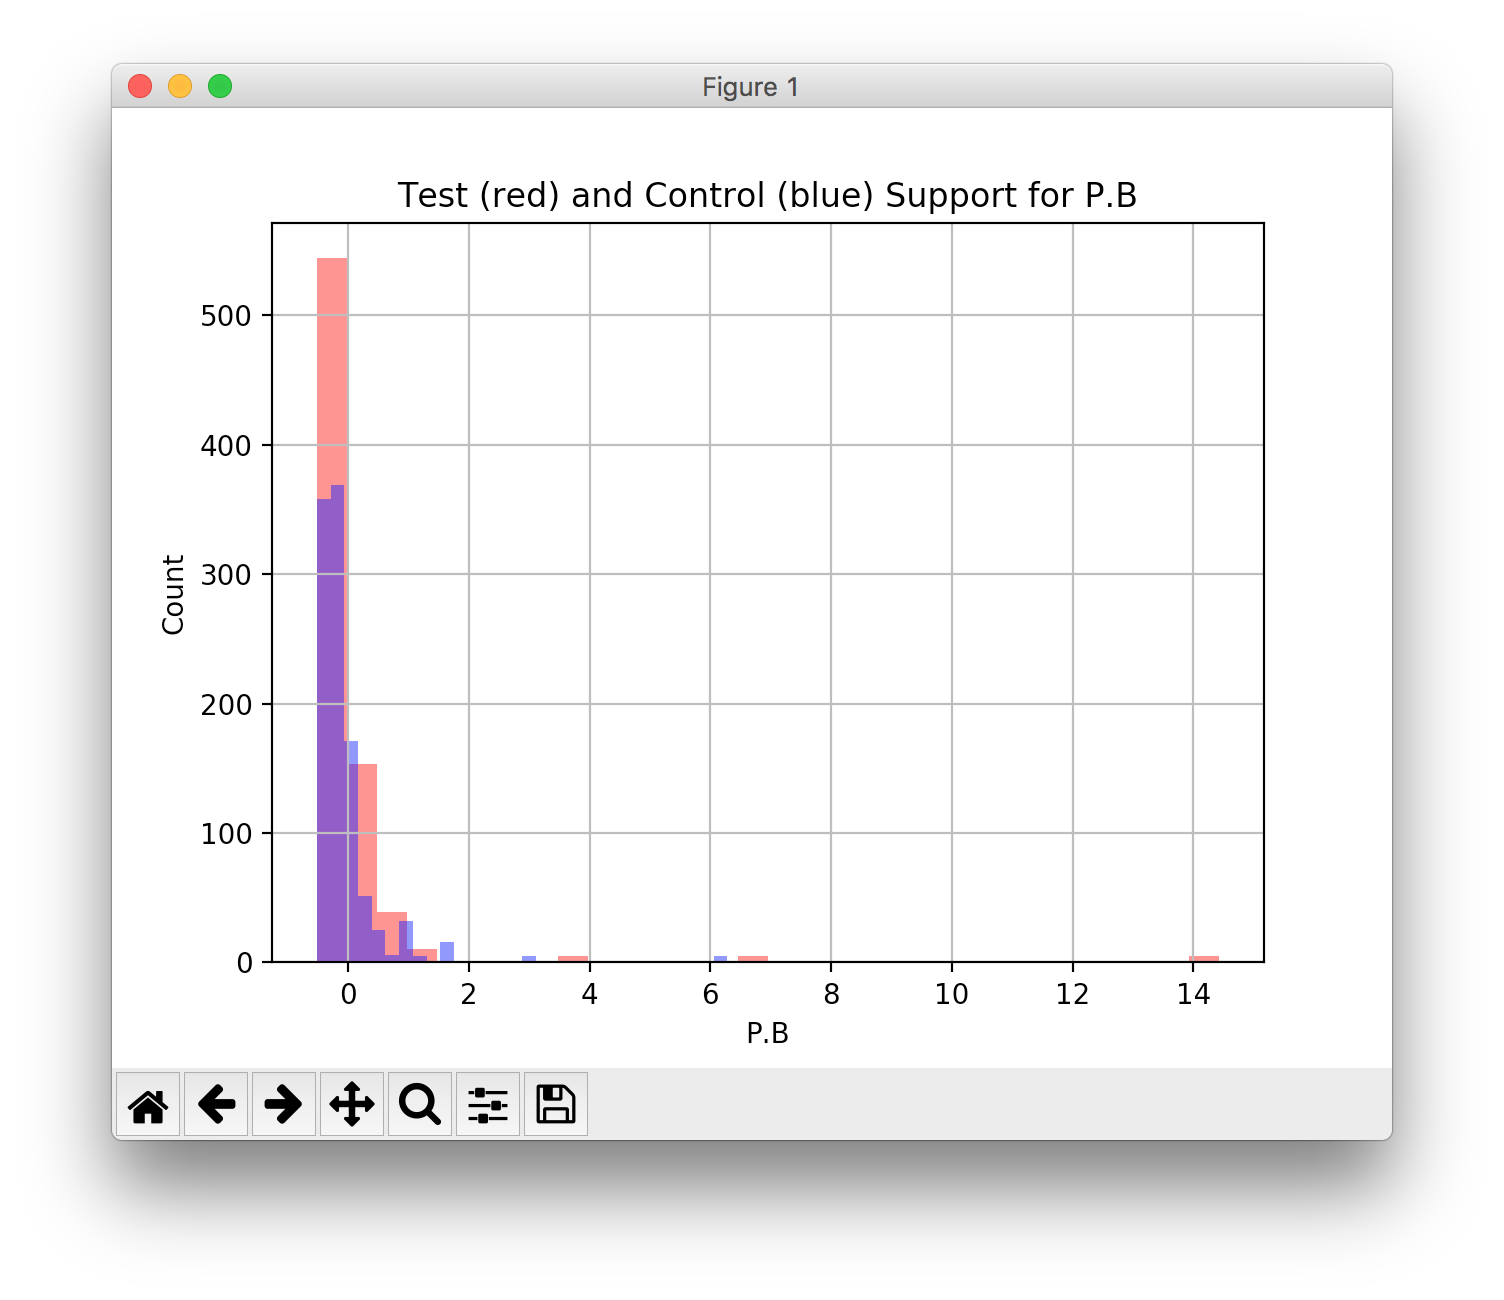
\includegraphics[width = 1.6in]{results/casual/BOD_Age_Rng/spx/tobin/P_B.png}} &
\subfigure[P/EBITDA]{\includegraphics[width = 1.6in]{results/casual/BOD_Age_Rng/spx/tobin/P_EBITDA.png}} \\
\subfigure[ROC]{\includegraphics[width = 1.6in]{results/casual/BOD_Age_Rng/spx/tobin/ROC.png}} 
\end{tabular}
\caption{Causal Estimation - Board of Directors Average Age}
\end{figure}
%\begin{figure}[h!]
%\begin{tabular}{ccc}
%\subfigure[caption]{\includegraphics[width = 1.5in]{results/casual/BOD_Age_Rng/altman/Asset.png}} &
%\subfigure[caption]{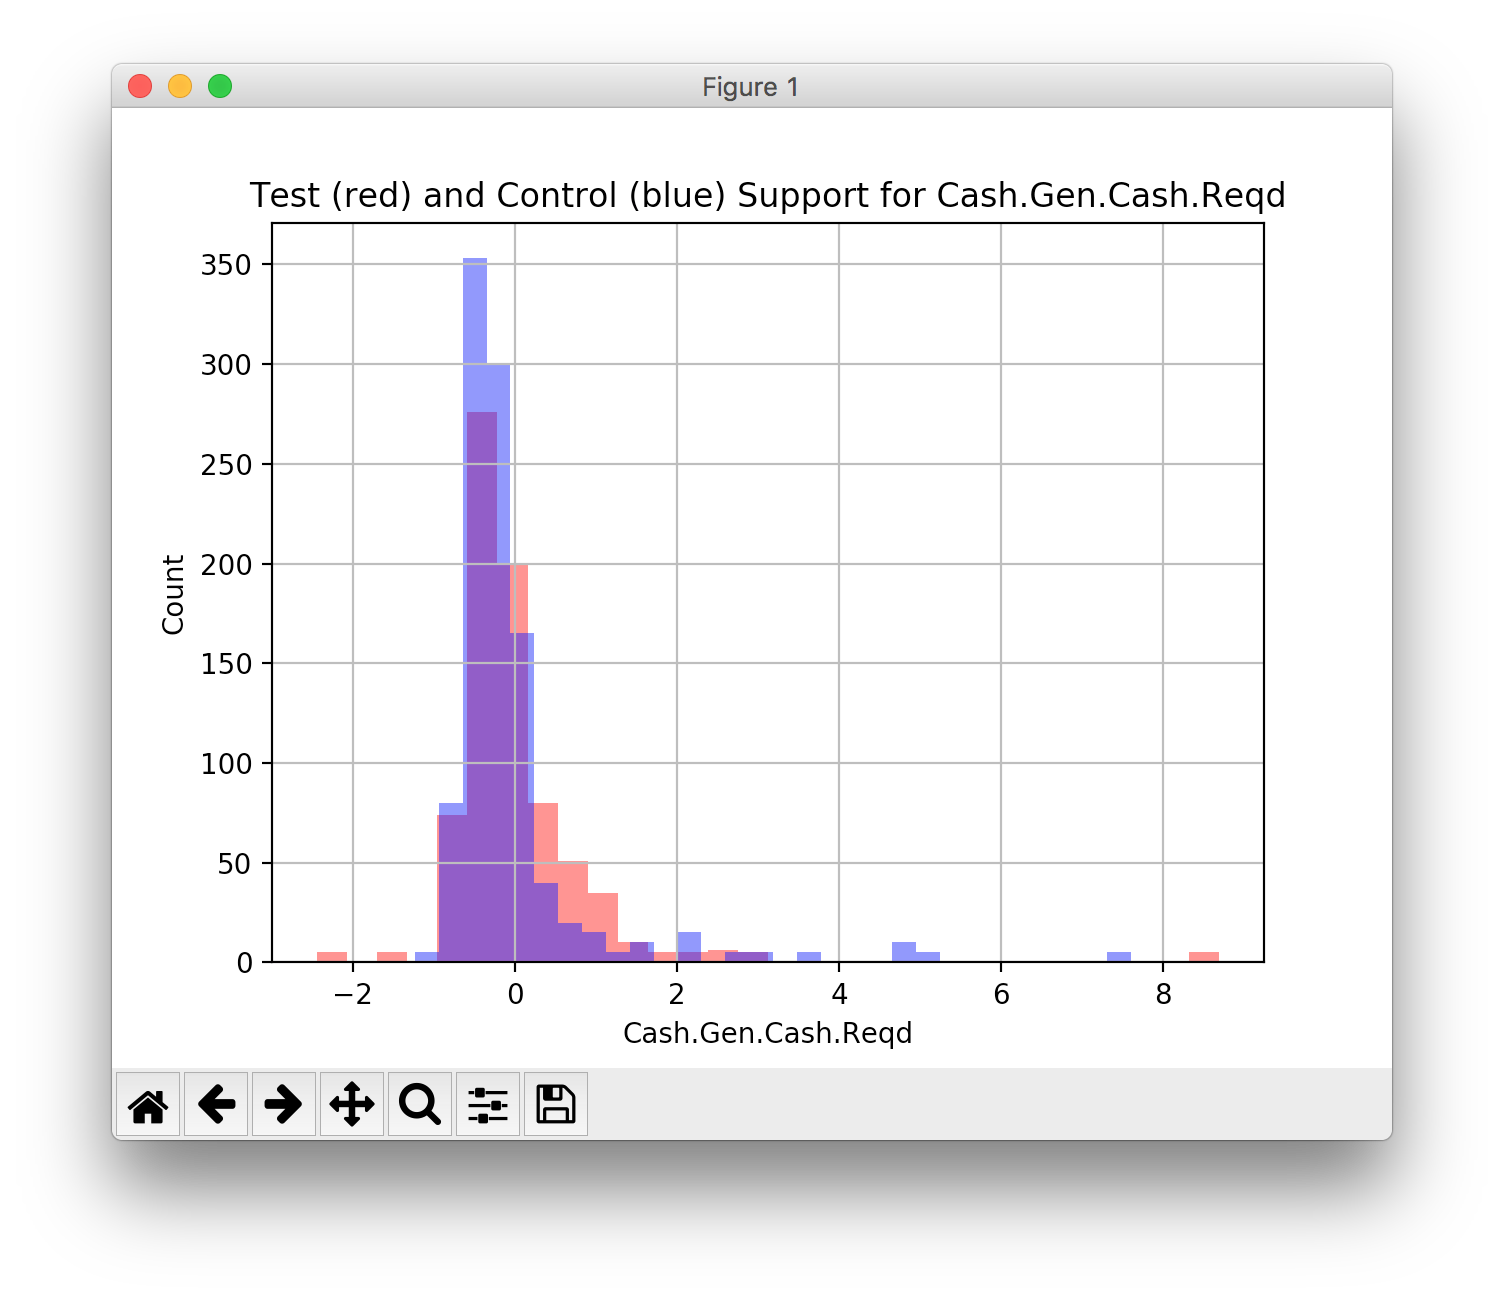
\includegraphics[width = 1.5in]{results/casual/BOD_Age_Rng/altman/Cash_Gen_Cash_Reqd.png}} &
%\subfigure[caption]{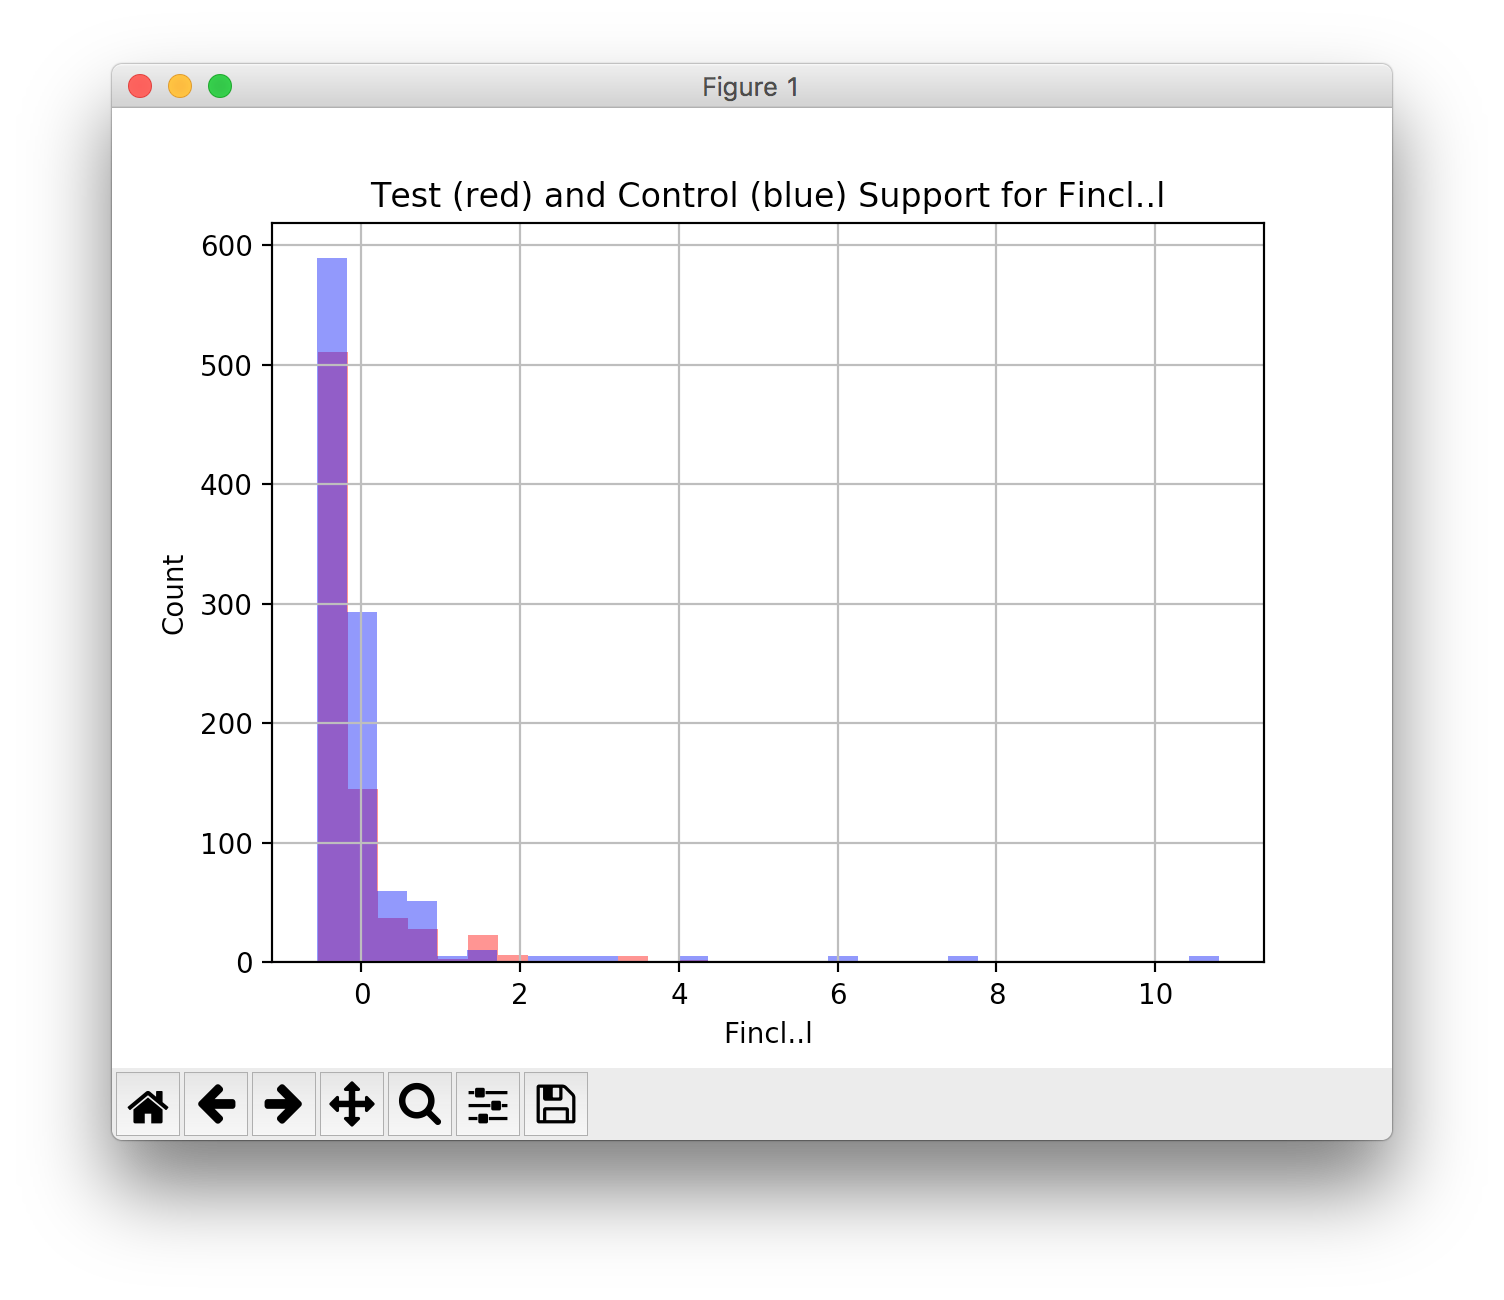
\includegraphics[width = 1.5in]{results/casual/BOD_Age_Rng/altman/Finc.png}} \\
%\subfigure[caption]{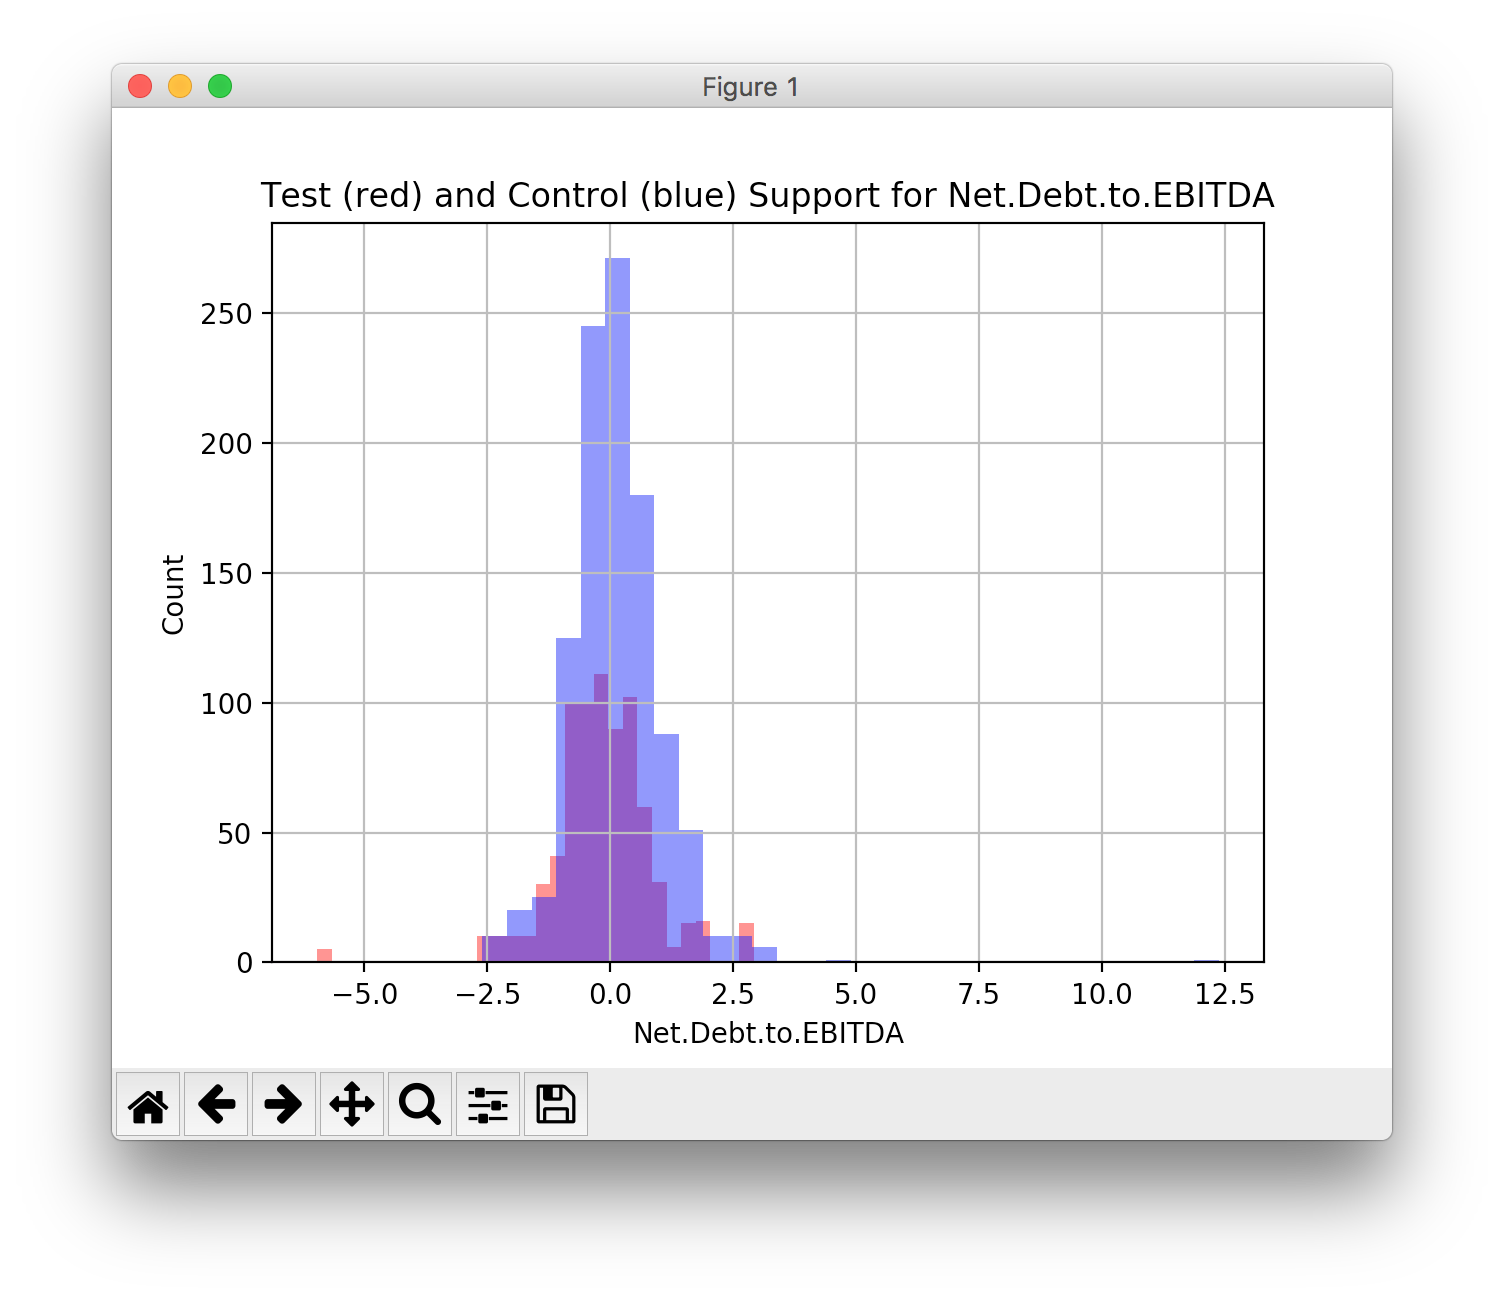
\includegraphics[width = 1.5in]{results/casual/BOD_Age_Rng/altman/Net_Debt_to_EBITDA.png}}&
%\subfigure[caption]{\includegraphics[width = 1.5in]{results/casual/BOD_Age_Rng/altman/P_EBITDA.png}} &
%\subfigure[caption]{\includegraphics[width = 1.5in]{results/casual/BOD_Age_Rng/altman/ROC.png}} \\
%\subfigure[caption]{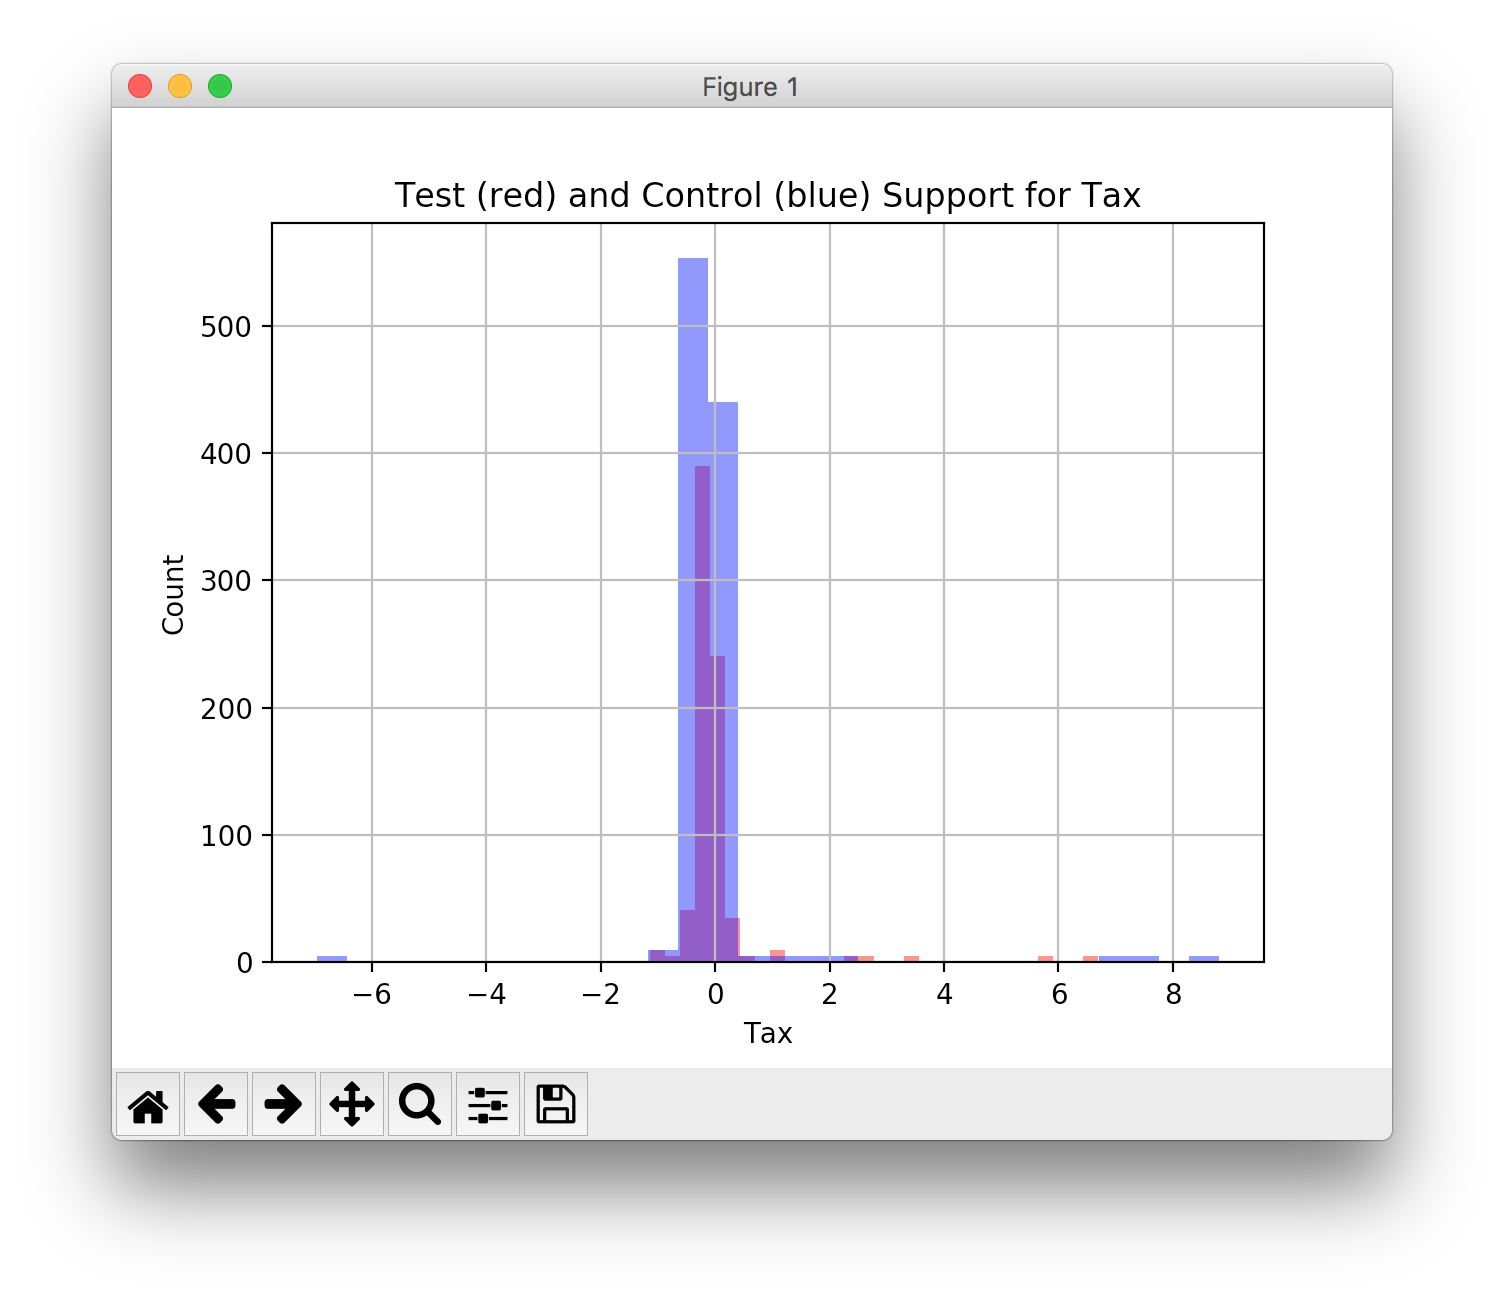
\includegraphics[width = 1.5in]{results/casual/BOD_Age_Rng/altman/Tax.png}} 
%\end{tabular}
%\caption{BOD.Age.Rng / Altman Z}
%\end{figure}
%{\bf Interval: } {(-0.009396477985696941, 0.012910009798425024, 0.037424725502139398)}
%\clearpage
%\fi
\clearpage

%%%%%%%%%%%%
%%Social Disclosure
%%%%%%%%%%%%
\subsubsection{Social Disclosure Score}
%\iffalse
\begin{tabular}{ll}
{\bf Market} & S\&P 500  \\
{\bf Outcome} & Altman Z Score \\
{\bf Treatment} & \footnotesize{Social Disclosure $>$ mean(Social Disclosure) ? 1 : 0 } \\
{\bf Motivating Statement} & \ref{wildTwo} [agrees, NA ]  \\
{\bf Estimate ($\% \Delta , 95\% \ CI$)} &  (0.04 , 0.09 , 0.14) \\~\\
{\bf Matching Plots} &
\end{tabular}
\begin{figure}[h!]
\begin{tabular}{ccc}
\subfigure[Asset]{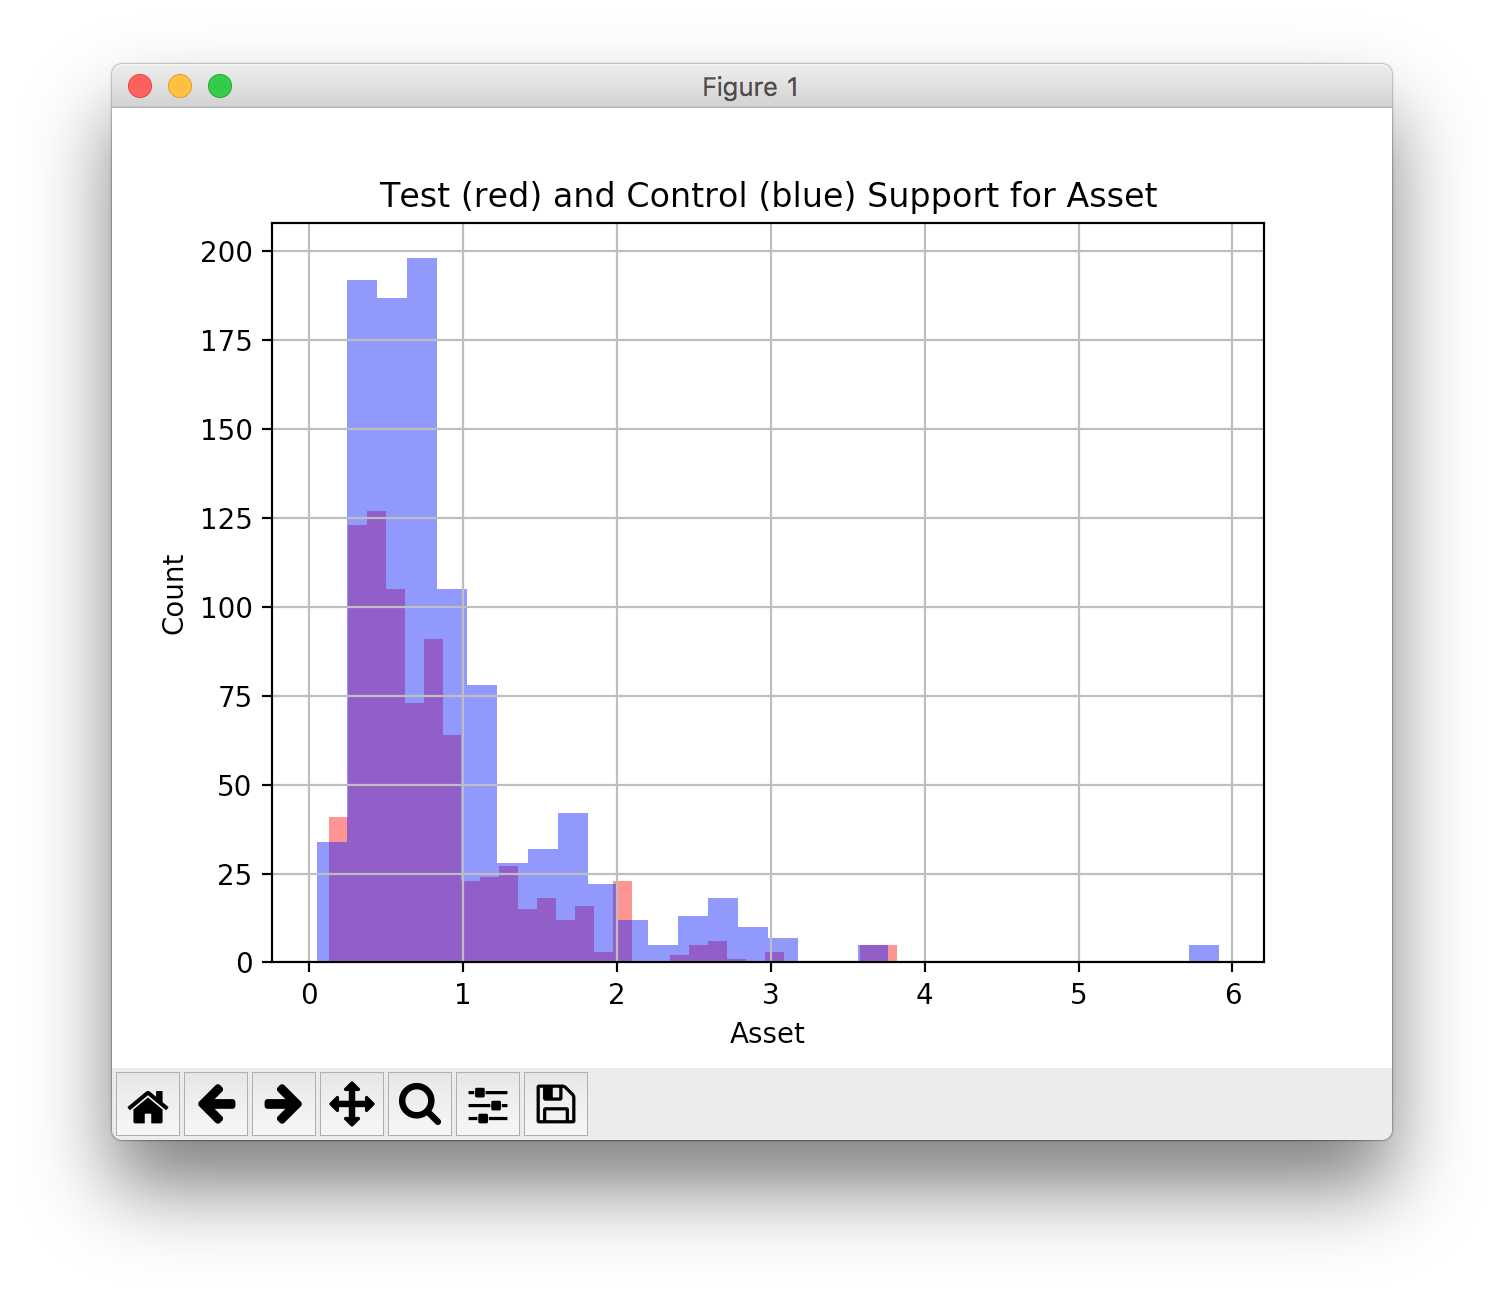
\includegraphics[width = 1.6in]{results/casual/socDis/spx/altman/asset.png}} &
\subfigure[Cash Gen/Cash Reqd]{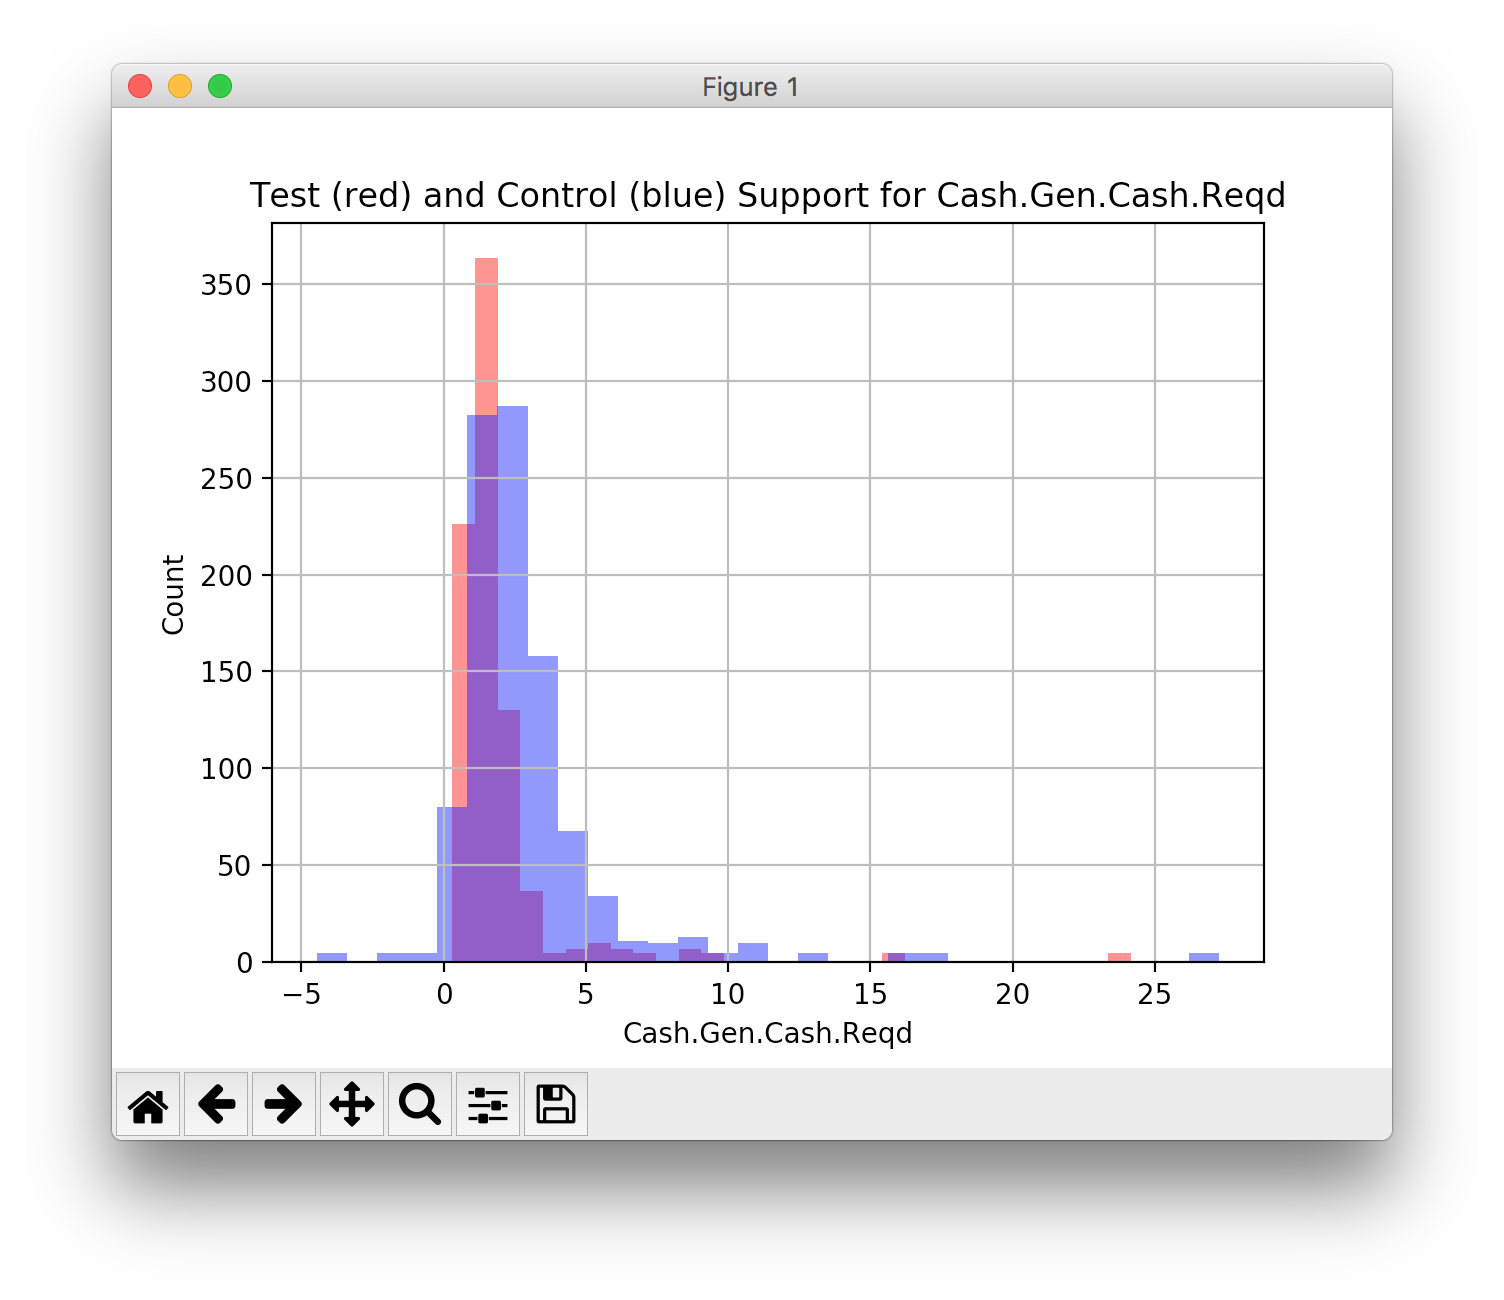
\includegraphics[width = 1.6in]{results/casual/socDis/spx/altman/cash_gen_cash_reqd.png}} &
\subfigure[Interest]{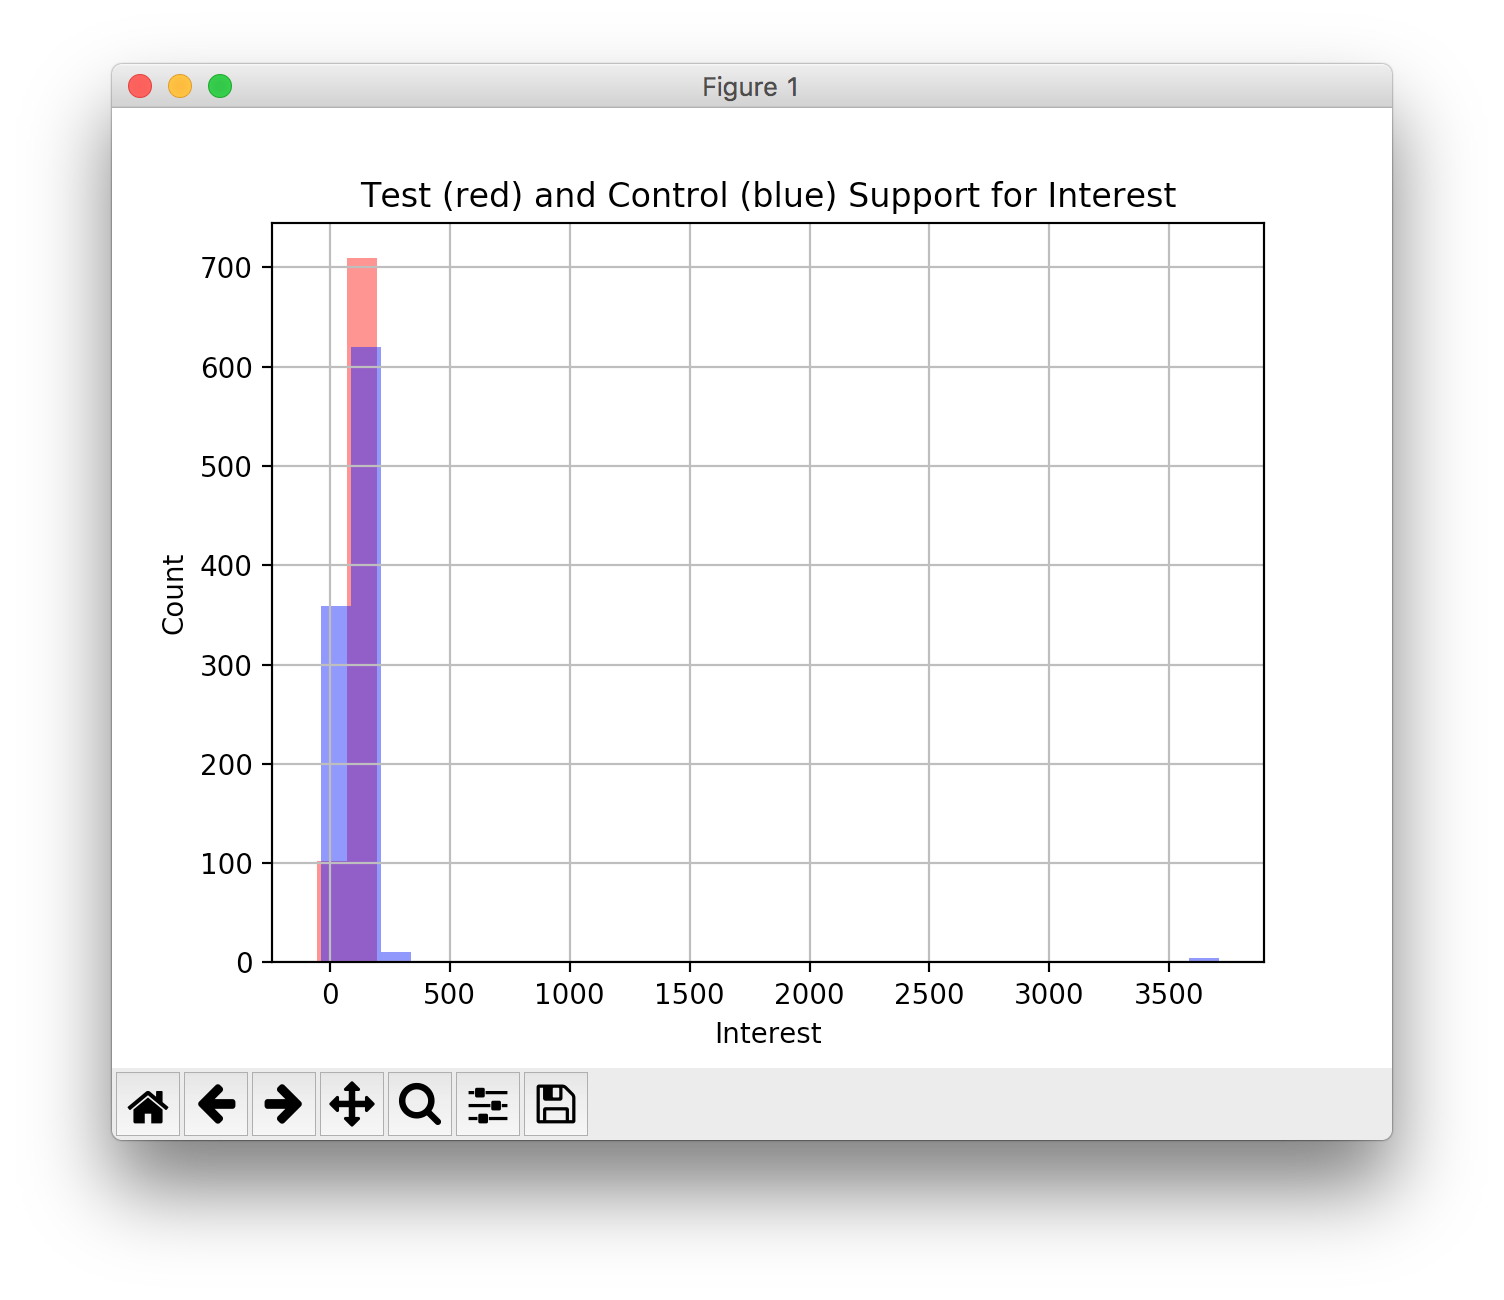
\includegraphics[width = 1.6in]{results/casual/socDis/spx/altman/interest.png}} \\
\subfigure[Fin Lev]{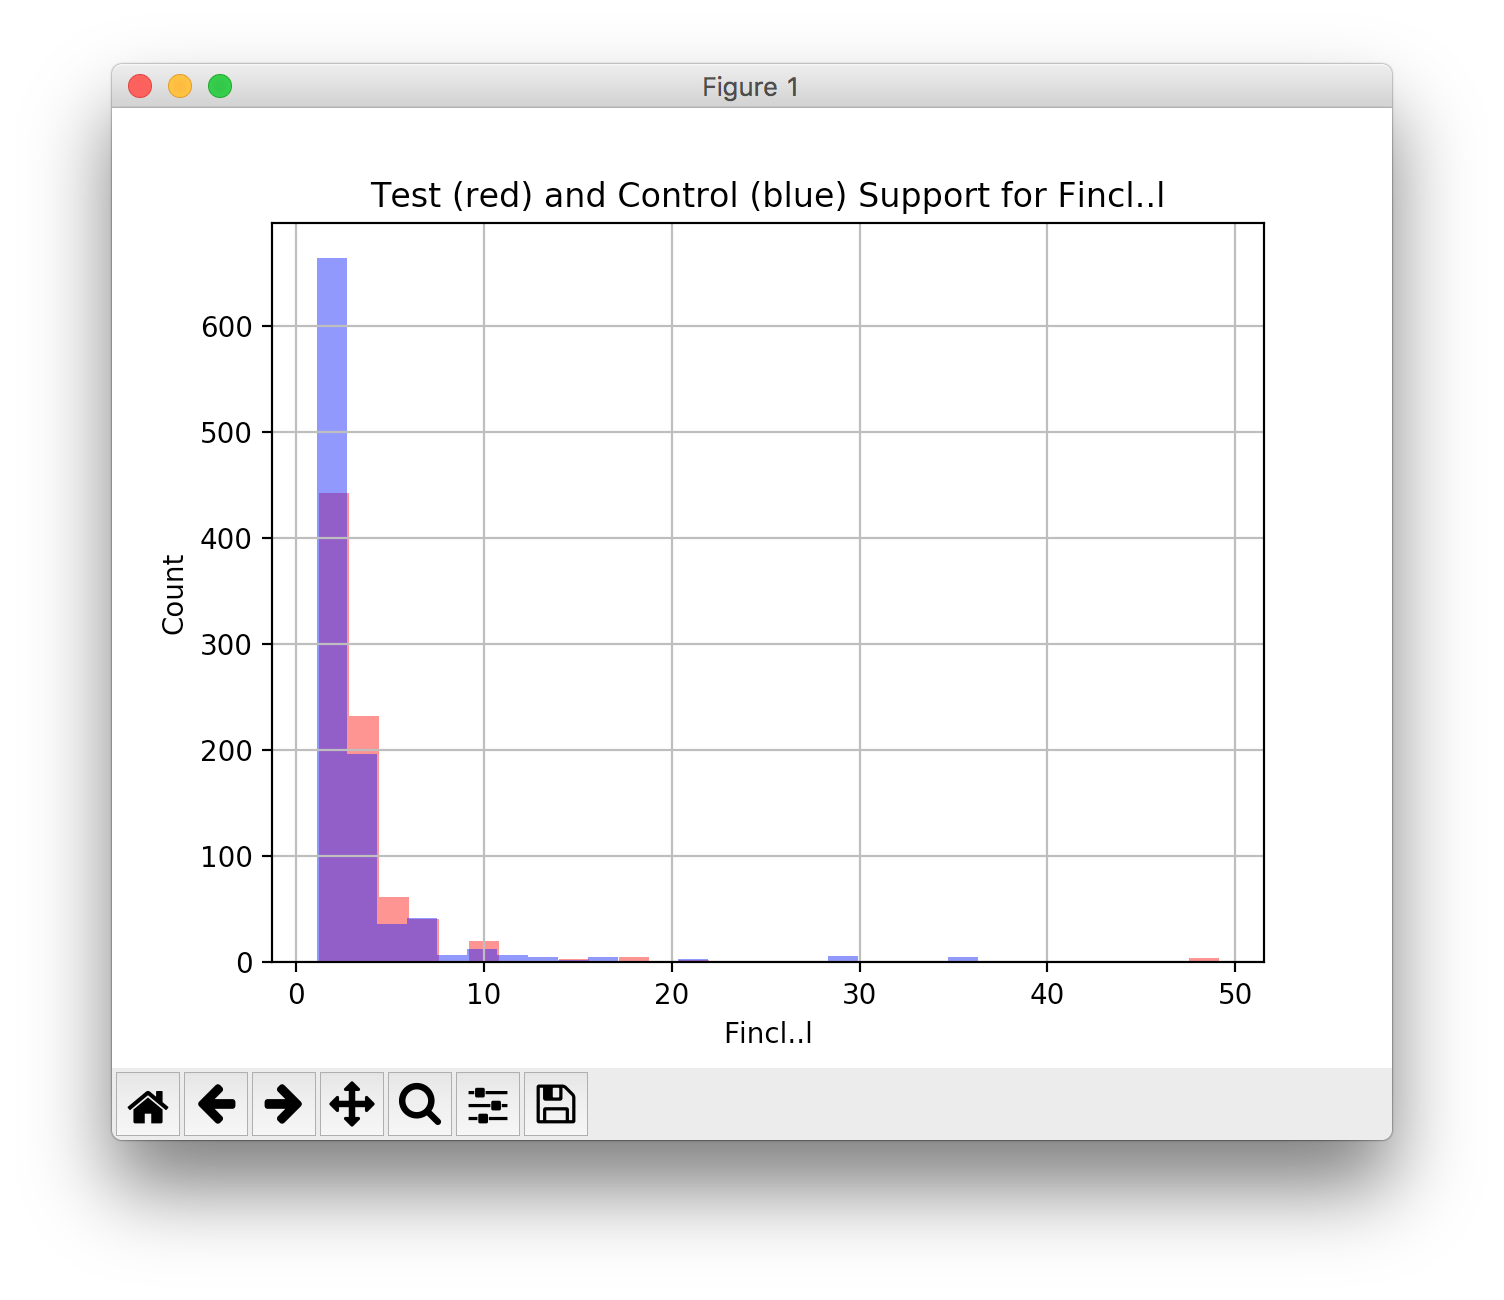
\includegraphics[width = 1.6in]{results/casual/socDis/spx/altman/fincl.png}} &
\subfigure[Net Debt/EBITDA]{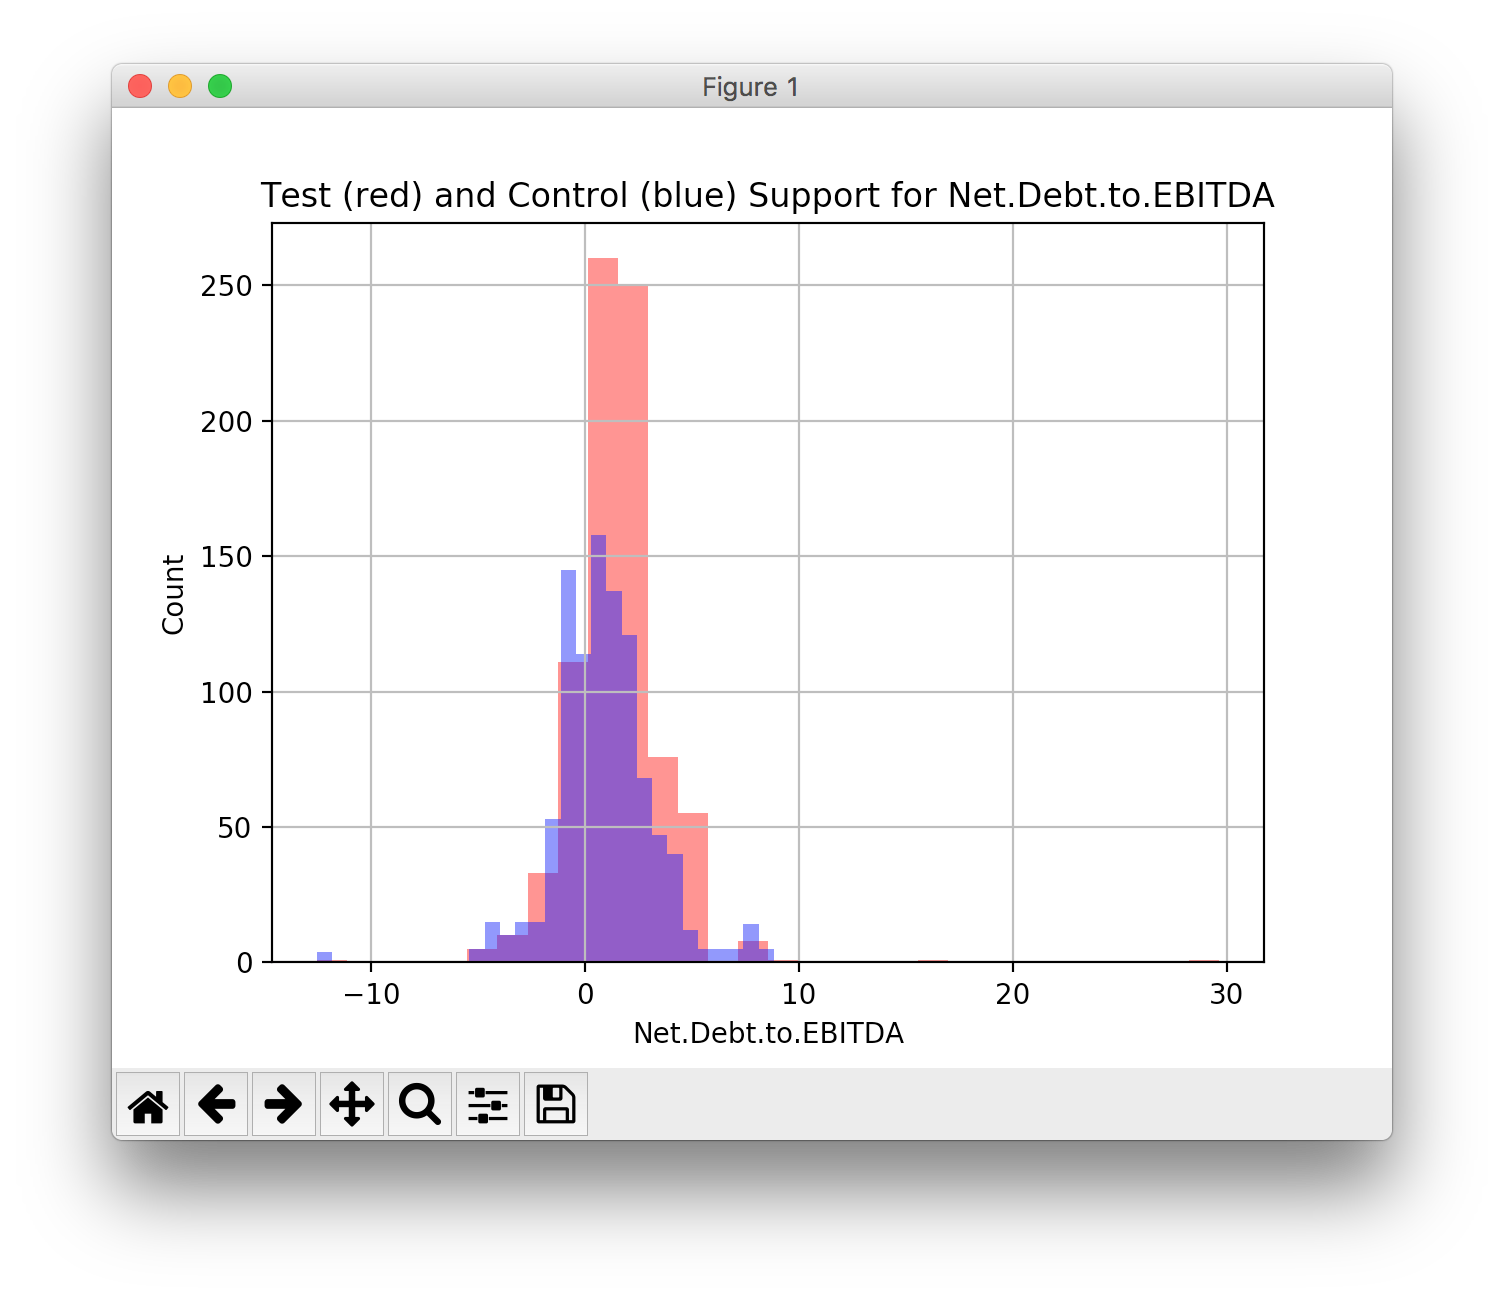
\includegraphics[width = 1.6in]{results/casual/socDis/spx/altman/net_debt_to_ebitda.png}} &
\subfigure[OPM 12Mth]{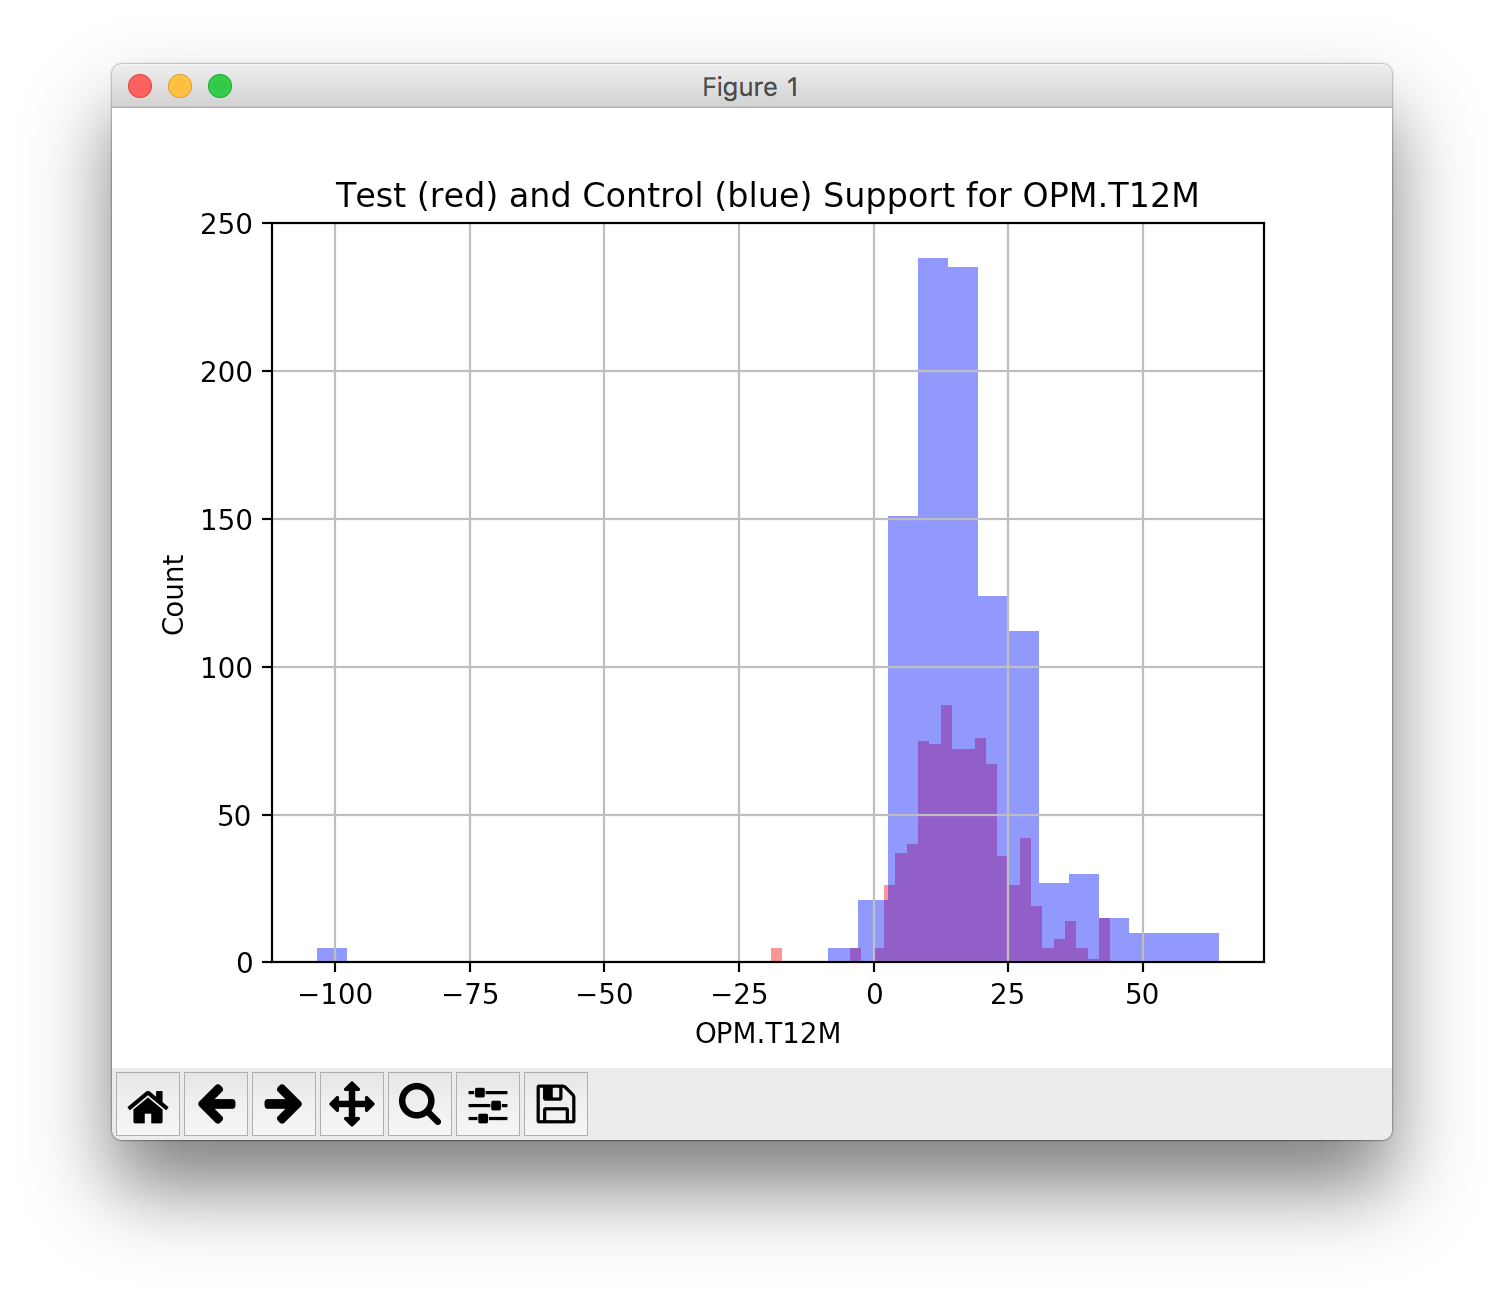
\includegraphics[width = 1.6in]{results/casual/socDis/spx/altman/opm_t12m.png}} \\
\subfigure[P/B]{\includegraphics[width = 1.6in]{results/casual/socDis/spx/altman/pb.png}} &
\subfigure[P/EBITDA]{\includegraphics[width = 1.6in]{results/casual/socDis/spx/altman/p_ebitda.png}} &
\subfigure[Tax]{\includegraphics[width = 1.6in]{results/casual/socDis/spx/altman/tax.png}} \\
\end{tabular}
\caption{Causal Estimation - Social Disclosure}
\end{figure}
%\fi 
\clearpage




\subsection{STOXX Europe 600}
%%%%%%%%%%%%
%%IFemale Board Members
%%%%%%%%%%%%
\subsubsection{Female Board Membership}
%\iffalse
\begin{tabular}{ll}
{\bf Market} & STOXX Europe 600  \\
{\bf Outcome} & Tobin's Q Score \\
{\bf Treatment} & {\% Female's on Board  $>$  20\%? 1 : 0 } \\
{\bf Motivating Statement} & \ref{westTwo} [disagrees, original], \ref{spOne} [agrees, not original]  \\
{\bf Estimate ($\% \Delta , 95\% \ CI$)} &  (0.06, 0.1, 0.14) \\~\\
{\bf Matching Plots} &
\end{tabular}
\begin{figure}[h!]
\begin{tabular}{ccc}
\subfigure[Asset]{\includegraphics[width = 1.5in]{results/casual/women_board/sxxp/tobin/Asset.png}} &
\subfigure[Net Debt/EBITDA]{\includegraphics[width = 1.5in]{results/casual/women_board/sxxp/tobin/Net_dedt_to_ebitda.png}} &
\subfigure[Fin Lev]{\includegraphics[width = 1.5in]{results/casual/women_board/sxxp/tobin/fincl.png}} \\
\subfigure[Norm NI to NI for Cmn]{\includegraphics[width = 1.5in]{results/casual/women_board/sxxp/tobin/norm_ni_to_ni_for_cmn.png}} &
\subfigure[Oper ROE]{\includegraphics[width = 1.5in]{results/casual/women_board/sxxp/tobin/oper_roe.png}} &
\subfigure[P/B]{\includegraphics[width = 1.5in]{results/casual/women_board/sxxp/tobin/PB.png}} \\
\subfigure[OPM 12Mth]{\includegraphics[width = 1.5in]{results/casual/women_board/sxxp/tobin/opm_t12m.png}}  &
\subfigure[P/EBITDA]{\includegraphics[width = 1.5in]{results/casual/women_board/sxxp/tobin/p_ebitda.png}}  &
\subfigure[AVG Adj ROE]{\includegraphics[width = 1.5in]{results/casual/women_board/sxxp/tobin/x5yr_avg_adj_roe.png}} 
\end{tabular}
\caption{Causal Estimation - Female Board Membership}
\end{figure}
%\fi
\clearpage

%%%%%%%%%%%%
%%indepDirFormerCEOBoard
%%%%%%%%%%%%
\subsubsection{Independent Director or Former CEO on the Board}
%\iffalse
\begin{tabular}{ll}
{\bf Market} & STOXX Europe 600  \\
{\bf Outcome} & Tobin's Q Score \\
{\bf Treatment} & {(Indep Director $\mid$  Former CEO on Board)? 1 : 0 } \\
{\bf Motivating Statement} & \ref{westOne} [disagrees, original]  \\
{\bf Estimate ($\% \Delta , 95\% \ CI$)} &  (0.30 , 0.35 , 0.40) \\~\\
{\bf Matching Plots} &
\end{tabular}
\begin{figure}[h!]
\begin{tabular}{ccc}
\subfigure[Asset]{\includegraphics[width = 1.5in]{results/casual/indepDirFormerCEOBoard/sxxp/tobin/Asset.png}} &
\subfigure[EPS]{\includegraphics[width = 1.5in]{results/casual/indepDirFormerCEOBoard/sxxp/tobin/EPS.png}} &
\subfigure[Fin Lev]{\includegraphics[width = 1.5in]{results/casual/indepDirFormerCEOBoard/sxxp/tobin/Fincl.png}} \\
\subfigure[Net Debt/EBITDA]{\includegraphics[width = 1.5in]{results/casual/indepDirFormerCEOBoard/sxxp/tobin/net_debt_to_ebitda.png}} &
\subfigure[OPM 12Mth]{\includegraphics[width = 1.5in]{results/casual/indepDirFormerCEOBoard/sxxp/tobin/OPM_T12M.png}} &
\subfigure[P/B]{\includegraphics[width = 1.5in]{results/casual/indepDirFormerCEOBoard/sxxp/tobin/PB.png}} \\
\subfigure[P/E]{\includegraphics[width = 1.5in]{results/casual/indepDirFormerCEOBoard/sxxp/tobin/PE.png}}  &
\subfigure[EV/EBITDA]{\includegraphics[width = 1.5in]{results/casual/indepDirFormerCEOBoard/sxxp/tobin/ev_ebitda.png}}  &
\subfigure[Avg Adj ROE]{\includegraphics[width = 1.5in]{results/casual/indepDirFormerCEOBoard/sxxp/tobin/X5Yr_avg_adj_roe.png}} 
\end{tabular}
\caption{Causal Estimation - Indep Director or Former CEO on the Board}
\end{figure}
%\fi
\clearpage

%%%%%%%%%%%%
%%Independent Director \& Financial Leverage
%%%%%%%%%%%%
\subsubsection{Independent Director \& Financial Leverage}
%\iffalse
\begin{tabular}{ll}
{\bf Market} & STOXX Europe 600  \\
{\bf Outcome} & Altman Z Score \\
{\bf Treatment} & \footnotesize{(Indep Lead Dir \& Financial Leverage $>$ 2.5)? 1 : 0 } \\
{\bf Motivating Statement} & \ref{spTwo} [agrees, not original]  \\
{\bf Estimate ($\% \Delta , 95\% \ CI$)} &  (-0.30 , -0.27 , -0.24) \\~\\
{\bf Matching Plots} &
\end{tabular}
\begin{figure}[h!]
\begin{tabular}{ccc}
\subfigure[Asset]{\includegraphics[width = 1.6in]{results/casual/indepDirFinlL/sxxp/altman/Asset.png}} &
\subfigure[Cash Gen/Cash Reqd]{\includegraphics[width = 1.6in]{results/casual/indepDirFinlL/sxxp/altman/Cash_Gen_Cash_Reqd.png}} &
\subfigure[Interest]{\includegraphics[width = 1.6in]{results/casual/indepDirFinlL/sxxp/altman/Interest.png}} \\
\subfigure[Fin Lev]{\includegraphics[width = 1.6in]{results/casual/indepDirFinlL/sxxp/altman/Fincl.png}} &
\subfigure[Net Debt/EBITDA]{\includegraphics[width = 1.6in]{results/casual/indepDirFinlL/sxxp/altman/Net_Debt_to_EBITDA.png}} &
\subfigure[P/E]{\includegraphics[width = 1.6in]{results/casual/indepDirFinlL/sxxp/altman/PE.png}} \\
\subfigure[P/B]{\includegraphics[width = 1.6in]{results/casual/indepDirFinlL/sxxp/altman/PB.png}} &
\subfigure[P/EBITDA 12Mth]{\includegraphics[width = 1.6in]{results/casual/indepDirFinlL/sxxp/altman/P_EBITDA_T12M.png}} &
\subfigure[Avg Adj ROE]{\includegraphics[width = 1.6in]{results/casual/indepDirFinlL/sxxp/altman/X5Yr_Avg_Adj_ROE.png}} 
\end{tabular}
\caption{Causal Estimation - Independent Director \& Financial Leverage}
\end{figure}
%\fi
\clearpage


\subsection{STOXX Eastern Europe 300}
%%%%%%%%%%%%
%%Indep.Chrprsn.Feml.CEO.or.Equiv
%%%%%%%%%%%%
\subsubsection{Independent Chairperson or Female CEO or Equivalent}
%\iffalse
\begin{tabular}{ll}
{\bf Market} & STOXX Eastern Europe 300  \\
{\bf Outcome} & Altman Z Score \\
{\bf Treatment} & {(Indep Chairman $\mid$  Female CEO)? 1 : 0 } \\
{\bf Motivating Statement} & \ref{eastThree} [agrees, original]  \\
{\bf Estimate ($\% \Delta , 95\% \ CI$)} &  (0.24, 0.29, 0.34) \\~\\
{\bf Matching Plots} &
\end{tabular}
\begin{figure}[h!]
\begin{tabular}{ccc}
\subfigure[Asset]{\includegraphics[width = 1.5in]{results/casual/Indep_Chrprsn_Feml_CEO_or_Equiv/sxxp/tobin/Asset.png}} &
\subfigure[EV/EBITDA]{\includegraphics[width = 1.5in]{results/casual/Indep_Chrprsn_Feml_CEO_or_Equiv/sxxp/tobin/EV_EBITDA.png}} &
\subfigure[Fin Lev]{\includegraphics[width = 1.5in]{results/casual/Indep_Chrprsn_Feml_CEO_or_Equiv/sxxp/tobin/Fincl.png}} \\
\subfigure[Net Debt/EBITDA]{\includegraphics[width = 1.5in]{results/casual/Indep_Chrprsn_Feml_CEO_or_Equiv/sxxp/tobin/Net_Debt_to_Ebitda.png}} &
\subfigure[OPM 12Mth]{\includegraphics[width = 1.5in]{results/casual/Indep_Chrprsn_Feml_CEO_or_Equiv/sxxp/tobin/OPM_T12M.png}} &
\subfigure[P/B]{\includegraphics[width = 1.5in]{results/casual/Indep_Chrprsn_Feml_CEO_or_Equiv/sxxp/tobin/PB.png}} \\
\subfigure[P/E]{\includegraphics[width = 1.5in]{results/casual/Indep_Chrprsn_Feml_CEO_or_Equiv/sxxp/tobin/PE.png}}  &
\subfigure[ROC]{\includegraphics[width = 1.5in]{results/casual/Indep_Chrprsn_Feml_CEO_or_Equiv/sxxp/tobin/ROC.png}}  &
\subfigure[Avg Adj ROE]{\includegraphics[width = 1.5in]{results/casual/Indep_Chrprsn_Feml_CEO_or_Equiv/sxxp/tobin/X5Yr_Avg_Adj_ROE.png}} 
\end{tabular}
\caption{Causal Estimation - Indep Chairperson or Female CEO (or Equiv)}
\end{figure}
%\fi
\clearpage






